\documentclass[11pt]{report}

\title{Teoria dei gruppi di Lie e approccio gruppale alla meccanica classica}
\author{AMM}


\usepackage{amsmath}
\usepackage{amsfonts}
\usepackage[mathscr]{eucal} 
\usepackage[utf8]{inputenc}
\usepackage[italian]{babel}
\usepackage{listings}
\usepackage{textcomp}
\usepackage{graphicx}
\usepackage{subfigure}
\usepackage{caption}
\usepackage{latexsym}
\usepackage{epstopdf}
\usepackage{eepic,epic,eepicemu}
\usepackage{color}

\usepackage[all]{xy}


\usepackage{bm}
\pagestyle{plain}
\definecolor{listinggray}{gray}{0.9}
\definecolor{lbcolor}{rgb}{0.95,0.95,0.95}

\usepackage{amsthm}

\usepackage[a4paper,top=4.25cm,bottom=3.75cm,left=4cm,right=2cm]{geometry}

\theoremstyle{plain}
\newtheorem{thm}{Teorema}[section]
\newtheorem{cor}[thm]{Corollario}
\newtheorem{lem}[thm]{Lemma}
\newtheorem{prop}[thm]{Proposizione}

\theoremstyle{definition}
\newtheorem{defn}{Definizione}[chapter]

\theoremstyle{remark}
\newtheorem{oss}{Osservazione}
\newcommand{\HRule}{\rule{\linewidth}{0.5mm}}

\begin{document}


\begin{titlepage}




\begin{center}
{\Huge Università degli Studi di Milano Bicocca}
\\[.1cm]
{\huge Facoltà di Scienze  Matematiche Fisiche e Naturali}
\\[.5cm]
{\huge Corso di Laurea in Fisica}
\\[1.5cm]

\includegraphics[keepaspectratio]{./immagini/logo}
\\[1.5cm]
\HRule \\[0.4cm]
{\huge \textbf{Teoria dei gruppi di Lie e applicazione alla meccanica del corpo rigido.}}
\HRule \\[1.5cm]


\begin{minipage}{0.4\textwidth}
\begin{flushleft} \large
{\Large \emph{Relatore:}}\\
{\Large Franco \textsc{Magri}}
\end{flushleft}
\end{minipage}
\begin{minipage}{0.4\textwidth}
\begin{flushright} \large
{\Large \emph{Tesi di Laurea di:}} \\
{\Large AM \textsc{M}} \\
{\large matricola: 072838}
\end{flushright}
\end{minipage}

\vfill

% Bottom of the page
{\Large Anno Accademico 2009 / 2010}
\end{center}

\end{titlepage}

%\maketitle


\begin{abstract}
Lo scopo di questo elaborato è la presentazione di una particolare applicazione della teoria dei gruppi di Lie alla meccanica classica.

Nello specifico si intende dimostrare come la riduzione delle equazioni del moto di un corpo rigido con punto fisso alle equazioni di Eulero sia connaturata alla struttura gruppale posseduta dallo spazio di configurazione del sistema.

Si comincia illustrando in modo astratto le principali caratteristiche della struttura di gruppo di Lie e la loro realizzazione per un generico gruppo di matrici.

In seguito viene presentato il gruppo delle rotazioni al fine di sottolineare il suo rapporto con lo spazio di configurazione del corpo rigido e con le sue possibili parametrizzazioni.

A questo punto ci sono tutti i presupposti per poter analizzare nello specifico la dinamica del corpo rigido.Dopo avere presentato brevemente la derivazione usuale, essenzialmente dovuta a Poisson, delle equazioni di Eulero, viene mostrata la loro traduzione nel linguaggio gruppale in due differenti modi.

Il primo modo consiste nel riconoscimento, nel sistema delle equazioni di Eulero, delle componenti dell'azione coaggiunta della velocità angolare sulla 1-forma momento angolare.

Nel secondo modo si fa riferimento all' \emph{equazione centrale della dinamica} di Lagrange e si dimostra come le equazioni di Eulero non siano altro che la proiezione di questa particolare equazione sulla base delle 1-forme invarianti a destra, oggetti legati univocamente alla natura gruppale dello spazio di configurazione del sistema.

Questo particolare risultato ha il pregio di poter essere esteso ad un qualsiasi sistema meccanico conservativo, a condizione che il suo spazio di configurazione sia un gruppo di Lie. Le equazioni che scaturiscono da questo processo sono dette \emph{equazioni di Eulero-Poincarè}.
\end{abstract}

\tableofcontents


\chapter{Teoria (in Astratto) dei gruppi di Lie}
\section{Introduzione}

\begin{defn}[\textbf{Gruppo}]$\\$
Insieme $G$ dotato di un'operazione $m$ :
$$m: G \times G \longrightarrow G \: \qquad \: m(g,h):=gh$$

tale per cui:

\begin{enumerate}
   \item $m$ soddisfa la proprietà associativa:
   $$ (gh)k=g(hk) \quad \forall g,h,k \in G$$
	\item elemento unità:
	$$\exists \, e \, \in G \qquad \textrm{t.c.} \qquad g = eg= ge \quad \forall g\in G $$ 
	\item elemento inverso:
	$$ \forall g\in G \quad \exists \, g^{-1} \qquad \textrm{t.c.} \qquad g g^{-1} = g^{-1} g = e  $$ 
\end{enumerate}

\end{defn} 


\begin{defn}[\textbf{Varietà Differenziale}]$\\$
Spazio Topologico M dotato di un atlante di carte compatibili.
\end{defn} 

\begin{defn}[\textbf{Gruppo di Lie}]$\\$
Varietà differenziabile G dotata della struttura di gruppo tale che la funzione $m$ di composizione e la funzione di inversione $(\cdot)^{-1}: \: g \mapsto g^{-1}$ siano regolari.
\end{defn}

\begin{defn}[\textbf{Algebra di Lie}]$\\$
Spazio vettoriale $V$ dotato di una funzione bilineare 
$$[\cdot,\cdot] : V \times V \rightarrow V$$
detta \emph{Bracket} tale che:

\begin{enumerate}
	\item antisimmetria:
   $$ [v,w]=-[w,v] \quad \forall v,w \in V$$
	\item identità di Jacobi:
	$$[[v,w],u] + [[u,v],w] + [[w,u],v] = 0 \quad \forall v,w,u \in V $$ 
\end{enumerate}

\end{defn}


\section{Strutture dei Gruppi di Lie}
\subsection{Le Traslazioni}
L'operazione di composizione $m$ di cui è munito G permette di definire due semplici mappe.
Fissato $ g \in G$ sono definite:

\begin{defn}[\textbf{Traslazione  a Sinistra}]\label{def:traslsinistra}
$$ L_{g}: G \rightarrow G \qquad \textrm{t.c.} \qquad L_{g}(h) = m(g,h) $$
\end{defn} 

\begin{defn}[\textbf{Traslazione  a Destra}]\label{def:trasldestra}
$$ R_{g}: G \rightarrow G \qquad \textrm{t.c.} \qquad R_{g}(h) = m(h,g) $$
\end{defn} 

Chiaramente, una volta scelto un atlante di carte su G, l'operazione di composizione ammette una rappresentazione in coordinate:
 
\begin{table}[h]
\begin{center} 
\begin{tabular}{l c l }
$k$ & = & $m(g,h)$\\
 & $\downarrow$ &  \emph{\small rappresentazione in carta locale} \\
$z^{a}$ & = & $\phi^{a}(x^{i},y^{j})$ \\
\end{tabular}
\end{center}
\end{table} 




\begin{oss}$\\$
La definizione di Gruppo di Lie assicura che queste funzioni siano dei diffeomorfismi (funzioni invertibili, differenziabili e con inverso differenziabile).
Quindi una carta coordinata definita in un intorno di G può essere trasformata, attraverso la composizione con una traslazione, in una carta dell'intorno traslato.
\end{oss} 

$\\$\begin{oss}[ Interpretazione geometrica del gruppo di Lie ]$\\$
Il gruppo di Lie è la più semplice estensione (non lineare) del concetto di Spazio Affine.
In G, gruppo di Lie, dati due punti del gruppo $(h_{1}, h_{2})$, esiste sempre un terzo elemento $g$ del gruppo tale che
$$h_2 = g h_{1} \Longleftrightarrow g = h_{2} h_{1}^{-1}$$

Questo corrisponde alla proprietà degli spazi affini per cui ad ogni coppia di punti $(A_{1}, A_{2})$ è possibile associare un vettore $\vec{v}$ tale che $A_{2} = A_{1} + \vec{v}$ ovvero $ \vec{v} = A_{2}-A_{1}$.

Quindi, così come ad ogni punto $P$ è possibile associare il vettore posizione $\vec{OP} = P - O$, ad ogni punto $g$ del gruppo si associa la traslazione $L_{g}()$ tale che : $$ L_{g}(e) = g e = g$$

A differenza dello spazio affine in cui punti e vettori possono essere identificati solo dopo aver scelto un punto O come origine degli assi ( associazione univoca del punto $P$ con il vettore $\vec{OP}$), in un gruppo di Lie i due oggetti sono automaticamente identificati, il motivo è che in un Gruppo c'è l'elemento Identità fissato come privilegiato.
\end{oss}

\subsection{Traslazioni di Vettori}
Dalla teoria delle Varietà differenziali si definisce in modo intrinseco un vettore come una classe di moti equivalenti (appendice \ref{appendice:1}). E' quindi possibile identificare uno specifico vettore con la velocità di un arbitrario moto appartenente alla sua classe di equivalenza.
Siccome in un Gruppo di Lie è presente un'elemento privilegiato (l'identità), lo spazio tangente  in tale punto ($T_{e}G$) giocarè un ruolo particolaramente importante.

\begin{defn}[\textbf{Traslazione in $T_{g}G$ del vettore $\xi \in T_{e}G$}]$\\$
Sia $\xi$ la velocità in $e$ del moto $\gamma(t)$ tale che $\gamma(0) = e$, la traslazione di $\xi$ è quindi la velocità calcolata in $g$ del moto $g(t)= L_{g}\circ \gamma(t) = g \cdot \gamma(t)$ ottenuto traslando di $g$ il moto $\gamma(t)$.

\end{defn} 

In coordinate, ricordando che $\phi^{a}(x,y): \mathbb{R}^{n} \times \mathbb{R}^{n} \rightarrow \mathbb{R}^{n}$ è la rappresentazione in coordinate locali della legge di composizione del Gruppo di Lie, si ottiene l'espressione in coordinate del moto traslato 
$$g^{a}(t) = \phi^{a}(g^{i},\gamma^{i}(t))$$

e da qui la velocità del moto risulta:
$$\dot{g}^{a}(t) \Bigr|_{t=0} = \dfrac{\textrm{d}}{\textrm{d}t} \phi^{a}(g^{i},\gamma^{i}(t)) \Bigr|_{t=0} = 
							\dfrac{\partial}{\partial \gamma^{k}} \phi^{a}(g^{i},\gamma^{i}(0)) \dot{g}^{k}(0)$$
ovvero:
$$\dot{\textbf{g}} = \textrm{d}L_{g}(e) \cdot \xi$$			

riconoscendo che $\dfrac{\partial}{\partial \gamma^{k}} \phi^{a}(g^{i},\gamma^{i}(0))$ corrisponde alla matrice Jacobiana della funzione di traslazione a sinistra di $g$ valutata nell'identità $\gamma(0)=e$.

Quindi l'applicazione lineare definita dalla suddetta matrice è detta \emph{Differenziale della Traslazione a Sinistra}:
$$	\textrm{d}L_{g}(e): T_{e}G \rightarrow T_{g}G$$
con questo operatore è possibile individuare lo spazio tangente ad ogni punto a partire dal solo spazio tangente nell'identità.

Pertanto la struttura di gruppo identifica naturalmente una struttura di trasporto di vettori dallo spazio tangente all'identità allo spazio tangente in un punto generico e viceversa.


\subsection{1-forma di Maurer-Cartan}
Si tratta di un'applicazione che associa in modo univoco ad un qualsiasi vettore sul gruppo di Lie G un vettore nello spazio tangente all'identità $T_{e}G$ anche detto \emph{algebra del gruppo}.

\begin{defn}[\textbf{1-forma di Maurer-Cartan}]$\\$
$\forall g \in G, \forall \dot{g} \in T_{g}G$ è l'applicazione definita come:
$$ \sigma_{g}: T_{g}G \rightarrow T_{e}G \qquad \textrm{t.c.}\qquad \sigma_{g}(\dot{g)}= \textrm{d}L_{g}^{-1}(e) \cdot \dot{g} = \xi \in \mathfrak{g} $$
\end{defn} 

Sostanzialmente si tratta dell'inverso dell'applicazione di trasporto di vettori, è detta 1-forma in quanto funzione lineare definita sullo spazio tangente al gruppo a valori nello spazio vettoriale costituito dall'algebra del gruppo.


\subsection{Campi Invarianti}
Sfruttando l'operazione di trasporto a sinistra $ \textrm{d}L_{g}(e) $ definita $\forall g \in G $ è possibile associare a partire da un singolo vettore $ \xi \in T_{e}G$ un campo vettoriale sul gruppo $G$.

$\\$Formalmente: $\textrm{d}L_{g}(e) $ definisce l'isomorfismo $\lambda: T_{e}G\rightarrow \mathfrak{X}_{L}(G)$ tale che:
$$\forall \xi \in T_{e}G \qquad : \qquad \lambda(\xi)= X_{\xi}^{L} := \textrm{d}L_{g}(e) \cdot \xi$$

Dove con $\mathfrak{X}(G)$ si indica l'insieme di tutti i campi vettoriali regolari si $G$ e con $\mathfrak{X}_{L}(G)$ il sottoinsieme dei campi invarianti a sinistra (più precisamente costituisce un sottospazio vettoriale).
$\\$In modo analogo, sfruttando la traslazione a destra, si può definire $\mathfrak{X}_{R}(G)$ il sottospazio dei campi invarianti a destra.

In conclusione i campi invarianti costituiscono una famiglia privilegiata di campi, isomorfi allo spazio $T_{e}G$
In questa ottica, il più generico vettore $(g,\dot{g}) \in TG$ può essere visto come elemento di un campo invariante quindi può essere associato ad un vettore dell'algebra, l'1-forma di Maurer-Cartan è appunto l'operazione che compie tale identificazione.

\subsection{1-forme invarianti}
In generale si intende per \emph{1-forma} sulla varietà differenziale $Q$ un qualsiasi funzionale lineare $TQ \rightarrow \mathbb{R}$, in altre parole si tratta di una funzione che associa ad ogni coppia punto vettore della varietà uno scalare.

\begin{defn}[\textbf{1-forma invariante}]$\\$
Particolare 1-forma $\mu: TQ \rightarrow \mathbb{R} $ associata ai campi invarianti $X_{\xi}^{L} $ (vale chiaramente sia per i campi a destra che per i campi a sinistra), tale che:
$$\mu (X_{\xi}^{L}  ) = \mu ( x, X_{\xi}^{L}(x)  ) = \mu_{\xi} \in \mathbb{R} \qquad \forall x \in Q\, , \, \forall \xi \in \mathfrak{g}$$
\end{defn} 

Pertanto una 1-forma si dice invariante se assume valore costante su ogni campo invariante, il valore dipende esclusivamente dal campo e non dal punto in cui viene calcolata.

\section{L'Algebra di un Gruppo di Lie}\label{chap:algebralie}
Si può individuare una relazione tra i gruppi di Lie e le Algebre in astratto.

Programma:
\begin{enumerate}
	\item Si dimostra che per ogni generica varietà differenziale $M$ lo spazio vettoriale $\mathfrak{X}(M)$ di tutti i campi vettoriali definiti su di essa costituisce un'algebra assieme al bracket di Lie-Jacobi. (appendice \ref{appendice:2})
	\item Sulla varietà di gruppo di Lie è definita una famiglia privilegiata di campi vettoriali, detti campi invarianti, che ha la proprietà di essere isomorfa a $T_{e}G$.
	\item Si dimostra che i campi invarianti a sinistra con il bracket di lie-jacobi costituiscono una sottoalgebra.
	\item Conclusione: $\\$ siano $\xi,\eta \in T_{e}G$ e $G$ gruppo di lie; siano $X_{\xi} , X_{\eta} \in \mathfrak{X}_{L}(G)$ i relativi campi invarianti.
	
	Definendo il \emph{ bracket di Lie} sullo spazio vettoriale $T_{e}G$ come $$ [\xi, \eta]_{\small (Lie)} := [X_{\xi}, X_{\eta}]_{\small (Jacobi-Lie)}(e)$$
	Siccome $\mathfrak{X}_{L}(G)$ costituisce un'algebra con $[\cdot,\cdot]_{\small{ (Jacobi-Lie)}}$ segue che $T_{e}G$ con $[\cdot,\cdot]_{\small (Lie)}$ formano una particolare algebra detta \emph{L'Algebra di Lie del Gruppo}.
	
	Per questo lo spazio $T_{e}G$ è anche detto l'algebra del gruppo e viene indicato con $\mathfrak{g}$.
\end{enumerate}

\begin{defn}[\textbf{Coefficienti di Struttura}]$\\$
Si consideri una base $\lbrace \xi_{i} \rbrace$ dell'algebra $\mathfrak{g}$ e siano $X_{i}$ i campi invarianti invarianti a sinistra ad essa associati. Si definiscono \emph{coefficienti di struttura} dell'algebra le quantità scalari $C_{i \, j}^{k} $ tali per cui
\begin{displaymath}
[X_{i} , X_{j} ] = C_{\: i \, j}^{k} \, X_{k}
\end{displaymath}
\end{defn}	
In sostanza sono i coefficienti che danno la decomposizione sulla base $\lbrace X_{k} \rbrace$ del campo che risulta dal commutatore di una coppia arbitraria di campi appartenenti alla base.

\begin{oss}$\\$
Si dimostra che il coefficiente ottenuto calcolando il commutatore nel caso dei campi invarianti a destra coincide con $ - \, C_{\: i\, j}^{k}$.
\end{oss}







\section{Strutture di Collegamento tra Algebra e Gruppo}

Siano $G$ gruppo di Lie , $ \mathfrak{g}$ l'algebra del gruppo e $ \mathfrak{X}_{\xi}$ il campo invariante a sinistra associato all'elemento $\xi \in \mathfrak{g}$.

\begin{defn}[\textbf{Sottogruppi ad 1 Parametro}]$\\$
Curva parametrizzata $\gamma_{\xi}(t) \subset G $ associata all'elemento $\xi \in \mathfrak{g}$ che soddisfa il sistema:
	\begin{displaymath}
	\left\{ 
			\begin{array}{rcl}
 			\dfrac{\textrm{d}\gamma_{\xi}}{\textrm{d}t} &=& X_{\xi}(g)\\& & \\	
 			\gamma_{\xi}(0) &=& e \\
  			\end{array} \right.
	\end{displaymath}
In altre parole è una curva tangente in ogni punto al campo invariante di $\xi$ e passante per l'identità.
\end{defn} 

\begin{oss}$\\$
I sottogruppi ad 1 parametro costituiscono un legame fra $\mathfrak{g}$ e $G$. Ad ogni elemento $g \in \mathfrak{g}$ corrisponde una curva parametrizzata su $G$.
\end{oss} 

\begin{defn}[\textbf{Mappa Esponenziale}]$\\$
Funzione $exp: \mathfrak{g} \rightarrow G$ tale che $$ exp(\xi) := \gamma_{\xi}(1)$$
\end{defn} 

\begin{oss}$\\$
Essendo $\mathfrak{g}$ uno spazio vettoriale è possibile decomporre il generico elemento $\xi \in \mathfrak{g}$ su una base. Attraverso la mappa esponenziale è possibile estendere quasta possibilità ad elementi del gruppo.
\end{oss} 

\begin{thm}[Relazione tra sottogruppi ad 1 parametro e mappa esponenziale]$\\$
Te: $\qquad \forall t \in \mathbb{R}, \: \forall \xi \in \mathfrak{g} \qquad \textrm{exp}(t\xi) = \gamma_{\xi}(t) $
\proof
Sfruttando la definizione per cui:
$$ \textrm{exp}(t \xi) = \gamma_{t \xi} (1)$$ 
l'idea è di dimostrare che
$$\forall \tau \in \mathbb{R} \qquad \gamma_{t\xi}(\tau) = \gamma_{\xi}(t \tau)$$
da cui, nel caso particolare di $\tau = 1$ , si ricava la tesi : $ \gamma_{t \xi} (1) = \gamma_{\xi}(t)$.

Per dimostrare l'uguaglianza tra $\gamma_{t\xi}(\tau)$ e $\gamma_{\xi}(t \tau)$ basta dimostrare che entrambe le curve $g(t)$ soddisfino la stessa equazione differenziale del tipo della definizione (1.9).
Quindi, per il teorema di esistenza e unicità della soluzione, entrambe le curve devono coincidere $\forall \tau$.

$\\$\emph{Curva $\gamma_{t \xi}(\tau)$}:
$\forall t$ fissato, la curva $ \tau \rightarrow \gamma_{t \xi}(\tau)$ soddisfa, per la definizione (1.9), il sistema:
	\begin{displaymath}
	\left\{ 
			\begin{array}{rcl}
			\gamma_{t \xi}(0) &=& e \\ 		& & \\	
 			\dfrac{\textrm{d} \gamma_{t \xi}(\tau)}{\textrm{d}\tau} &=& X_{t \xi}\Bigr(\gamma_{t \xi}(\tau)\Bigr) = \textrm{d}L_{\gamma_{t \xi}(\tau)}(e) \cdot t \xi = t \cdot \textrm{d}L_{\gamma_{t \xi}(\tau)}(e) \xi = t \cdot X_{\xi}\Bigr(\gamma_{t \xi}(\tau)\Bigr) \\
 			\end{array} \right.
	\end{displaymath}
La penultima uguaglianza è data dalla linearità dell'operatore $\textrm{d}L_{g}(e)$.

$\\$\emph{Curva $\gamma_{\xi}(t \tau)$}:
$\forall t$ fissato, la curva $ \tau \rightarrow \gamma_{\xi}(t \tau)$ soddisfa il sistema:
	\begin{displaymath}
	\left\{ 
			\begin{array}{rcl}
			\gamma_{\xi}(0) &=& e \\ & & \\				
 			\dfrac{\textrm{d} \gamma_{\xi}(t \tau)}{\textrm{d}\tau} &=& t \cdot \dfrac{\textrm{d} \gamma_{\xi}(t \tau)}{\textrm{d}t\tau} = t \cdot X_{\xi}\Bigr(\gamma_{t \xi}(\tau)\Bigr) \\
 			\end{array} \right.
	\end{displaymath}
per il teorema di derivazione della funzione composta.

$\\$ Pertanto entrambe le curve soddisfano la stessa equazione differenziale.

\endproof
\end{thm} 




\begin{thm}[$\gamma_{\xi}(t)$ costituiscono effettivamente un gruppo]$\\$
Hp: Sia $\gamma_{\xi}$ una curva soluzione del problema
	\begin{displaymath}
	\left\{ 
			\begin{array}{rcl}
 			\dfrac{\textrm{d}\gamma_{\xi}}{\textrm{d}t} &=& X_{\xi}(g)\\& & \\	
 			\gamma_{\xi}(0) &=& e \\
  			\end{array} \right.
	\end{displaymath}
Te: $ \gamma_{\xi} ( t + s) = \gamma_{\xi}(s) \gamma_{\xi}(t) \qquad s,t \in \mathbb{R}$
\proof
Si identifichi la prima curva dell'uguaglianza come $g(t)$ e la seconda come $g'(t)$.
Si può dimostrare la tesi verificando che entrambe soddisfino la stessa equazione differenziale.
Dalla definzione di sottogruppo ad 1 parametro seguono le seguenti equazioni:
 	\begin{displaymath}
	g : \left\{ 
			\begin{array}{rcl}
			g(0) &=& \gamma_{\xi}(s + 0 ) \\ & & \\				
 			\dfrac{\textrm{d} g}{\textrm{d}t} &=& \dfrac{\textrm{d} (s + t)}{\textrm{d}t} \cdot \dfrac{\textrm{d} \gamma_{\xi}(k)}{\textrm{d}k} = X_{\xi} \Bigr( \gamma (t + s)\Bigr) = X_{\xi}(g) \\
 			\end{array} \right.
	\end{displaymath}

 	\begin{displaymath}
	g' : \left\{ 
			\begin{array}{rcl}
			g'(0) &=& \gamma_{\xi}(s) \cdot \gamma_{\xi}(t) \\ & & \\				
 			\dfrac{\textrm{d} g'}{\textrm{d}t} &=& \textrm{d}L_{\gamma_{\xi}(s)} \cdot \Bigr( \dfrac{\textrm{d} \gamma_{\xi}(t)}{\textrm{d}t} \Bigr) = \textrm{d}L_{\gamma_{\xi}(s)} X_{\xi} \Bigr(\gamma_{\xi}(t) \Bigr) = X_{\xi}\Bigr(\gamma_{\xi}(s) \cdot \gamma_{\xi}(t) \Bigr)\\
 			\end{array} \right.
	\end{displaymath}

L'ultima equazione è dedotta dal fatto che $g'(t)$ è la traslazione dell'elemento $\gamma_{\xi}(s) $ della curva $\gamma_{\xi}(t)$, pertanto la sua velocità è la velocità traslata.	

Ricordando che $\gamma_{\xi}(s) \cdot \gamma_{\xi}(t) = g'(t) $ si conclude che $g$ e $g'$ soddisfano le stesse equazioni differenziali.
	
\endproof
\end{thm} 

Da ciò si conclude che $\forall \xi \in \mathfrak{g}$ l'insieme $\{ exp(t\xi) | t \in \mathbb{R}\} = \{ \gamma_{\xi}(t)| t \in \mathbb{R}\}$ costituisce un sottogruppo ad 1 parametro nel senso dato dalla definizione.
Si può dimostrare anche il viceversa, ovvero che una qualsiasi curva $\gamma(t)$ che costituisce un sottogruppo di $G$, quindi tale per cui che $$\forall s,t \in \mathbb{R} \qquad \gamma(s)\gamma(t) = \gamma(s+t)$$ risolve il sistema differenziale della definizione (1.10). Quindi se $\xi$ è la sua velocità in $t=0$ può essere espressa come $\gamma_{\xi}(t) = exp (t \xi)$.
\proof
sia $\xi = \dot{\gamma}(0)$ allora:

\begin{displaymath}
\dfrac{\textrm{d} \gamma}{\textrm{d}t} = \dfrac{\textrm{d} \gamma}{\textrm{d}s}\bigr|_{s=0} \gamma(t+s) = \dfrac{\textrm{d} \gamma}{\textrm{d}s}\bigr|_{s=0} \gamma(t) \gamma(s) = \textrm{d}L_{\gamma(t)} \cdot \dot{\gamma(0)} = X_{\xi}(\gamma(t)) 
\end{displaymath}
Quindi soddisfa $\gamma$ soddisfa la definizione (1.9).
\endproof


\section{Le Azioni di un gruppo di Lie}
 \label{adg}
 Sia $G$ un gruppo di Lie e $M$ una varietà, si considera una generica funzione $\phi : G \times M \rightarrow M $ la cui rappresentazione, fissato un sistema di coordinate $x^{i}$ su $M$ e $g^{\alpha}$ su $G$, risulta:
$$ y^{i} = \phi^{i} ( x^{1}, \ldots, x^{m} ; g^{1}, \ldots, g^{k})$$
Si richiede che la legge $\phi$ che unisce elementi del gruppo e punti della varietà rappresenti il gruppo sulla varietà.

Quindi, fissato un elemento $g \in G$, riguardando $\phi$ come un'applicazione sulla varietà $M$ a valori in se stessa dipendente dalla scelta di $g$: $$\phi_{g} :M \rightarrow M$$
(quindi la si può intendere come una mappa che associa $\forall g \in G$ una funzione regolare $\phi_{g}$)

Si dice che $\phi$ è un'\emph{azione} ( oppure \emph{rappresentazione} nel caso la varietà M sia uno spazio vettoriale e $\phi_{g}$ sia lineare) se valgono due condizioni:

\begin{enumerate}
   \item $\phi_{e} = Id$
   \item $\phi_{g_{1}} \cdot \phi_{g_{2}} = \phi_{g_{1}\cdot g_{2}}$
\end{enumerate}

Più precisamente si definisce:

\begin{defn}[\textbf{Azione a sinistra del gruppo G sulla varietà M}]\label{def:azionegruppo}$\\$
Mappa regolare $\phi : G \times M \rightarrow M$ tale che:
\begin{enumerate}
   \item $\phi(e,x) = x \qquad \forall x \in M$
   \item $\phi(g,\phi(h,x)) = \phi(gh,x) \qquad \forall g,h \in G, \forall x\in M$
   \item $\forall g \in G$ la mappa $\phi_{g}:= \phi(g,x) : M \rightarrow M$ è un diffeomorfismo.
\end{enumerate}
\end{defn} 

\begin{oss}$\\$
Nel caso dell'\emph{Azione a Destra} la definizione è analoga con l'unica differenza che la condizione 2) diventa: 
$$\phi(g,\phi(h,x)) = \phi (hg,x) $$
\end{oss} 


 \subsection{Azioni di un Gruppo di Lie su se stesso}

\paragraph{Azione delle Traslazioni} $\\$
Su un gruppo di Lie sono definiti i 2 diffeomorfismi fondamentali delle traslazioni a destra e sinistra.
Ciascuna di esse può agire sia a destra che a sinistra.
\begin{table}[h!]
\begin{center}
\begin{tabular}{|c|c|c|}
\hline
 & Azione a Sinistra & Azione a Destra \\
 \hline
Traslazione a Sinistra & $(g,h) \rightarrow L_{g}(h) : = gh $ & $(g,h) \rightarrow L_{g^{-1}}(h) : = g^{-1}h $ \\
\hline
Traslazione a Destra & $(g,h) \rightarrow R_{g^{-1}}(h) : = h g^{-1} $ &  $(g,h) \rightarrow R_{g}(h) : = h g^{-1} $ \\
\hline
\end{tabular}
\end{center}
\end{table}  

Per convenzione si stabilisce che l'azione di $G$ su se stesso per \emph{Traslazione a Sinistra} è l'azione a sinistra di $L_{g}$ mentre l'azione di $G$ su se stesso per \emph{Traslazione a Destra} è l'azione a destra di $R_{g}$.
 
 \paragraph{Azione per Coniugazione} $\\$

Si tratta dell'applicazione che nasce componendo consecutivamente una traslazione a sinistra e una a destra.
Nello specifico è l'azione:

	\begin{displaymath}
G \times G \rightarrow G \qquad ; \qquad (g,h) \rightarrow I_{g} (h) := \bigr(L_{g} \cdot R_{g^{-1}}\bigr) (h) = g h g^{-1}
	\end{displaymath}

Dove la funzione $I_{g}$ è l'applicazione detta \emph{Inner Automorphism} che informalmente esce a sinistra da un intorno del punto $h$ e ritorna nell'intorno da destra.
In generale tale applicazione coincide con l'identità solo nell'intorno dell'elemento unità del gruppo.

\subsection{Azioni aggiunte sull'Algebra}

Sono le operazioni che nascono dalla composizione di una traslazione a sinistra e di una a destra consecutiva.

\paragraph{Azione aggiunta del gruppo sulla sua algebra} $\\$
Azione:
	
	\begin{displaymath}
G \times \mathfrak{g} \rightarrow \mathfrak{g} \qquad ; \qquad (g,\xi) \rightarrow Ad_{g} (\xi) :=  \dfrac{\textrm{d}}{\textrm{d}t} \bigr(I_{g}(\gamma(t)\bigr) \Bigr|_{ t=0}
	\end{displaymath}
Dove 
	\begin{displaymath}
	\gamma(t) = \left\{ 
			\begin{array}{rcl}
 			\gamma(0) &=& Id\\
 			\dot{\gamma}(0) &=& \xi \\
  			\end{array} \right.
	\end{displaymath}

In sostanza si tratta del differenziale di $I$ lungo una curva dotata di velocità $\xi$ nel punto $e$.
Dalla definizione (1.7) e dalla derivazione delle funzioni composte si può concludere che $\forall v \in \mathfrak{g}$ risulta:
	\begin{displaymath}
	Ad_{g}(v) = \textrm{d}R_{g^{-1}}(g)\textrm{d}L_{g}(e) \xi = \textrm{d}R_{g}^{-1}(e)\textrm{d}L_{g}(e)\xi
	\end{displaymath}
dove la seconda uguaglianza è valida in virtù del fatto che $ R_{g}^{-1}(e) = R_{g^{-1}}(g)$.

\paragraph{Azione aggiunta dell'algebra su se stessa} $\\$
Applicazione:
	\begin{displaymath}
\mathfrak{g} \times \mathfrak{g} \rightarrow \mathfrak{g} \qquad ; \qquad (\xi,\eta) \rightarrow ad_{\xi} (\eta) :=  \dfrac{\textrm{d}}{\textrm{d}t} Ad_{\textrm{exp}(t\xi)}\eta \Bigr|_{ t=0}
	\end{displaymath}

ovvero è il differenziale dell'azione aggiunta di un elemento $\eta$ dell'algebra calcolato lungo la curva ad un parametro associato all'elemento $\xi$.

\paragraph{Azione Coaggiunta dell'algebra sul suo duale} $\\$
Applicazione $ ad^{\ast}: \mathfrak{g} \times \mathfrak{g}^{\ast} \rightarrow \mathfrak{g}^{\ast}$ tale che $\forall \xi \in \mathfrak{g}$ la mappa $ad^{\ast}_{\xi}:\mathfrak{g}^{\ast} \rightarrow \mathfrak{g}^{\ast} $ è il duale dell'operatore di azione aggiunta:

	\begin{displaymath}
< ad_{\xi}^{\ast} \mu , \eta > = < \mu , ad_{\xi} \eta > \qquad \forall \xi , \eta \in \mathfrak{g} \: \forall \mu \in \mathfrak{g}^{\ast}
	\end{displaymath}
dove con $< \mu, \eta> $ si intende $\mu(\eta)$ ovvero l'applicazione della 1-forma $\mu$ sul vettore $\eta$. Questa notazione allude alla possibilità di identificazione tra algebra e suo duale in presenza di un prodotto interno.

 \subsection{Generatori Infinitesimali}

Si consideri l'azione a sinistra di un gruppo di Lie $G$ sulla varietà differenziale $M$:
$$ \phi(g,x) \rightarrow g x \qquad \forall g \in G, \; \forall x \in M$$

\begin{defn}[\textbf{Orbita passante per $x$}]$\\$
Fissato $x \in M$ è il luogo dei punti $\textrm{orb}(x) \subseteq M$ tale che:
$$\textrm{orb}(x) :=  \{ g x : g \in G\}$$
\end{defn} $\\$

Si consideri inoltre $\xi \in \mathfrak{g}$ , vettore dell'algebra del gruppo, e il sottogruppo ad 1 parametro $ \{ exp(t \xi) : t \in \mathbb{R} \} \subseteq G $ ad esso associato.
Allora l'orbita di un'elemento $x$ rispetto a questo sottogruppo sarà un cammino reale:
$$ t \rightarrow \Bigr( exp(t \xi) \Bigr) x $$

\begin{defn}[\textbf{Generatore Infinitesiamale}]$\\$
Vettore $\bm{\xi}_{M}(x)$ tangente nel punto $x$ al cammino $\Bigr( exp(t \xi) \Bigr) x \subset M$. Esplicitamente:
$$\bm{\xi}_{M}(x) :=  \dfrac{\textrm{d}}{\textrm{d}t} \Bigr|_{t=0} \Bigr( exp(t \xi)x \Bigr)$$
\end{defn} $\\$
Si tratta di un vettore tangente alla varietà $M$ nel punto $x$ associato ad un particolare elemento $\xi \in \mathfrak{g}$ dell'algebra del gruppo che agisce su $m$.
Siccome fissato $\xi \in M$ è possibile associare un suo generatore per ogni $x \in M$, più sinteticamente si può affermare che tale elemento definisce su $M$ un campo di generatori $\bm{\xi}_{M}()$.






\clearpage

\chapter{Gruppi di Matrici}
Con gruppo di Matrici si intende un sottoinsieme di $\mathcal{M}(n,\mathbb{R}) $ o di $\mathcal{M}(n,\mathbb{C}) $ ( matrici quadrate $n \times n$ a valori reali o complessi) che costituisce un gruppo rispetto all'usuale prodotto tra matrici.
$\\$
\begin{oss}$\\$
Siccome per la definizione ogni insieme per essere un gruppo deve contenere l'inverso di ogni elemento, ogni gruppo di matrici è necessariamente un sottoinsieme di $\textrm{GL}(n, \mathbb{R})$, insieme delle matrici quadrate invertibili.
$\\$
Inoltre, visto che il prodotto tra matrici è associativo e la condizione per una matrice di essere invertibile è che il suo determinante sia non nullo, il teorema di Binet ( $\textrm{Det}(AB) = \textrm{Det}(A) \textrm{Det}(B)$) assicura che $\textrm{GL}(n, \mathbb{R})$ sia il più grande gruppo di matrici $ n \times n$.
\end{oss} 
$\\$
\begin{oss}$\\$
L'insieme delle matrici $n \times n$ con elementi reali è naturalmente isomorfo a $\mathbb{R}^{n^{2}} $ tramite l'associazione alla matrice della n-pla delle sue componenti.
Alla luce di questo lo studio dei gruppi di Lie di matrici si riduce al più immediato studio delle sottovarietà dello spazio euclideo, dove sia punti che vettori possono essere rappresenentati come elementi dello stesso spazio ambiente.
\end{oss} 
$\\$
Nel corrente capitolo si intenderà con $G$ un generico gruppo di Lie di Matrici, quindi:
$ G \subset \mathcal{M}(n,\mathbb{R}) $ e sottogruppo di Lie di $\textrm{GL}(n, \mathbb{R})$ con $m: G \times G \rightarrow G$ l'usuale prodotto tra matrici.


\paragraph{Traslazioni} $\\$
Dalla definizione in astratto si deduce che per $R\in G$, gruppo di matrici,  vale che:
$$L_{R}(\cdot) = m(R, \cdot) = R \cdot \qquad R_{R} = m(\cdot, R) = R_{R}(\cdot) = \cdot R$$


\section{Strutture tangenti ad un Gruppo di Matrici}
Per via dell'ambientazione del gruppo di matrici in $\mathcal{M}(n,\mathbb{R}) $ anche i vettori tangenti saranno matrici $ n \times n$ a valori reali.
$\\$Questo rende comodo prendere come rappresentante della classe di equivalenza definente il singolo vettore la curva:

	\begin{displaymath}
	A(t) = Id + t \dot{A} = \left\{ 
			\begin{array}{lcl}
 			A(0) &=& Id\\ & & \\
 			\dfrac{\textrm{d} A(t)}{\textrm{d}t} \Bigr|_{t=0} &=& \dot{A} \\
  			\end{array} \right.
	\end{displaymath}
che rappresenta una retta nello spazio ambiente ma appartiene al gruppo $G$ solo nell'intorno dell'elemento unità (per la precisione il suo sviluppo al primo ordine è contenuto nel gruppo), in altre parole si tratta di una retta tangente alla varietà $G$.
$\\$Il vettore è il valore dell velocità di questa curva parametrizzata con $t$ calcolato in $t=0$.

Pertanto si ottiene un procedimento per costruitre lo spazio tangente all'unità del gruppo di Lie, l'insieme di tutte le matrici $\dot{A}$ tali che $ A(t) $ è una retta tangente in $Id$ costituisce $T_{Id}G = \mathfrak{g}$.

\subsection{Traslazione di Vettori}
La traslazione, a sinistra , di un vettore $\dot{A}$ applicato in $Id$ in un punto $R \in G$ è la velocità della curva $\gamma(t)$ ottenuta traslando a sinistra di $R$ la curva  $A(t)$ definita nel paragrafo precedente.
Quindi:
	\begin{displaymath}
\gamma(t) =R \bigr( Id + t \dot{A} \bigr)  \qquad \dot{\gamma(t)} \Bigr|_{t=0} = R \dot{A} 
	\end{displaymath}
	\begin{displaymath}
\Longrightarrow \qquad \textrm{d}L_{R}(Id) \dot{A} = R\dot{A} = \dot{R}
	\end{displaymath}
Da cio si conclude che $\dot{A} = R^{-1}\dot{R}$ pertanto si può esplicitare la 1-forma di Maurer-Cartan (a sinistra) 
\begin{equation}\label{eq:maurercartansinistramatrici}
\Omega^{L}(\dot{R}) = \textrm{d}L_{R}^{-1}(Id) \cdot \dot{R} = R^{-1} \dot{R}
\end{equation}
con $R \in G$ e $\dot{R} \in T_{R}G$ e dove $R^{-1}$ è la matrice inversa nel senso del calcolo matriciale.

Analogamente è possibile estendere questo discorso per le traslazioni a destra ottenendo:
	\begin{equation}\label{eq:maurercartandestramatrici}
\textrm{d}R_{R}(Id) \dot{A} = \dot{A}R \qquad \Omega^{R}(\dot{R}) = \textrm{d}R_{R}^{-1}(Id) \cdot \dot{R} = \dot{R} R^{-1} 
	\end{equation}
con $R \in G, \, \dot{A}\in \mathfrak{g}$ e $\dot{R}\in T_{R}G$ generici elementi.

Una volta trovato l'insieme delle matrici formanti l'algebra di un gruppo, si può ottenere lo spazio tangente in ogni punto semplicemente applicando gli operatori di traslazione.	


\subsection{Algebra di un Gruppo di Matrici}
Applicando il procedimento espresso nel capitolo (\ref{chap:algebralie}) si cerca la forma esplicita per il commutatore nel caso di gruppi di Lie formati da matrici.

In questo caso i campi invarianti, elementi di $\mathfrak{X}_{L}\Bigr(GL(n)\Bigr)$ sono nella forma:
$$X_{A}(g) = \textrm{d}L_{g}(e) A = gA$$
dove $g \in G$ e $A \in T_{I}G$ sono entrambi matrici quadrate.

Per costruire il commutatore del gruppo di Lie è necessario poter esprimere i campi invarianti nella forma di operatori di derivazione di funzioni scalari.
Per semplicità ci si limita a considerare le sole funzioni $f:G \rightarrow \mathbb{R}$ lineari. A queste funzioni è possibile associare una matrice $F \in GL(n)$ tale che:
	\begin{displaymath}
f(G) = Tr \Bigr( F \cdot G \Bigr)
	\end{displaymath}
Quindi, dalla definizione di campo vettoriale come derivazione sulle funzione, segue che:
	\begin{displaymath}
X_{A}\emph{(f)}(g) = \dfrac{\textrm{d} }{\textrm{d}t} \Bigr(Tr \bigr(F\cdot G( 1 + tA) \bigr) \Bigr) \Bigr|_{t=0} = Tr \bigr(F\cdot( G A) \bigr) = Tr\bigr((AF)G \bigr) 
	\end{displaymath}
dove $f$ è la funzione scalare argomento della derivazione e $g$ e il punto in cui si calcola la direzione del campo invariante $X_{A}$.

E' evidente che $X_{A}\emph{(f)}(g) $ sia ancora una funzione scalare su $G$, pertanto è possibile calcolarne la derivata rispetto ad un secondo campo invariante $Y_{B} $:
	\begin{displaymath}
Y_{B} \Bigr(X_{A}\emph{(f)} \Bigr)(g) = \dfrac{\textrm{d} }{\textrm{d}t} \Bigr(Tr \bigr(AF\cdot G( 1 + tB) \bigr) \Bigr) \Bigr|_{t=0} = Tr \bigr(AFGB \bigr) = Tr\bigr(F\cdot G(BA) \bigr) 
	\end{displaymath}
Quindi, per un gruppo di matrici, il commutatore dei campi invarianti assume la forma:
	\begin{displaymath}\begin{split}
X_{A}\Bigr(Y_{B}\Bigr) - Y_{B}\Bigr(X_{A}\Bigr) \emph{(f)} (g) &=  Tr\bigr(F\cdot G(AB) \bigr)- Tr\bigr(F\cdot G(BA) \bigr) = \\ &= Tr\bigr(F\cdot G(AB - BA) \bigr) = X_{(AB - BA)} \emph{(f)} (g)
\end{split}	\end{displaymath}
Si conclude che per un gruppo di matrici il commutatore dell'algebra assume la forma:
\begin{equation}\label{eq:commutatorematrici}
[A,B] = AB-BA \qquad \textrm{con }\,  A,B \in T_{I}G
\end{equation}

\subsection{Generatori infinitesimali}
Nel caso dell'azione di un gruppo di matrici $G \subseteq GL(n, \mathbb{R})$ su uno spazio vettoriale $\mathbb{R}^n $ si definisce l'azione standard di un generico elemento $R$ del gruppo come:
	\begin{displaymath}
\phi(R,x)= R x 
	\end{displaymath}
con l'usuale applicazione di una matrice ad un vettore colonna, n-pla di $\mathbb{R}$.
In questo caso il generatore infinitesimale assume la particolarmente semplice espressione:
	\begin{displaymath}
\xi_{M}(x) = \dfrac{\textrm{d} }{\textrm{d}t} \Bigr|_{t=0} \Bigr( exp(t \xi)  x \Bigr) = \dfrac{\textrm{d} }{\textrm{d}t} \Bigr|_{t=0} = \xi x 
	\end{displaymath}
dove $\xi \in \mathfrak{g}$.

\subsection{Mappe esponenziali}
\begin{thm}[Mappa esponenziale per un gruppo di matrici]\label{teo:esponenzialematrici}$\\$
\begin{itemize}
	\item[-]IP: $G$ gruppo di lie di matrici
\item[-]Te: La mappa esponenziale $exp(A)$ con $A \in \mathfrak{g}$ definita sulla varietà coincide con la matrice esponenziale definita dal calcolo matriciale come:
$$e^{A} = Id +  \sum_{i=1}^{\infty}\frac{A^{i}}{i!}$$
\end{itemize}	

\proof
Dal calcolo è noto che $\forall A \in GL(n,\mathbb{R})$ si ha che $e^{A} \in GL(n,\mathbb{R})$, ovvero la serie dell'esponenziale converge ed è invertibile con $ (e^{A})^{-1} = e^{-A}$.
Pertanto $e^{\cdot}: GL \rightarrow GL$ è un'applicazione biunivoca.

Quindi l'insieme $\{ e^{t A}\: | \: t\in \mathbb{R} \: A \in \mathfrak{g} \}$ è una curva parametrizzata su $G$ di velocità :

\begin{displaymath}
\dfrac{\textrm{d}}{\textrm{d}t} e^{t A} = \frac{\textrm{d}}{\textrm{d}t}\sum_{i=1}^{\infty}\frac{(tA)^{i}}{i!} = A \sum_{n=1}^{\infty}\frac{(tA)^{n-1}}{(n-1)!} = A e^{tA} = e^{tA} A
\end{displaymath}
Ricordando che il campo invariante di $A \in \mathfrak{g}$ risulta $X_{A}^{L}(g) = \textrm{d}L_{g}(e) \cdot A = gA$ si trova che $\gamma_{A}(t) = e^{tA}\subset G$ soddisfa il problema:

\begin{displaymath}
	\left\{ 
			\begin{array}{rcl}
 			\gamma_{A}(0) &=& Id \\	
 			\dot{\gamma_{A}}(t) &=& \dfrac{\textrm{d}}{\textrm{d}t} e^{t A} = e^{tA} A = \textrm{d}L_{e^{tA}}(e)A = X_{A}(e^{tA})\\
  			\end{array} \right.
	\end{displaymath}

Pertanto la curva $e^{tA}$ è il sottogruppo ad 1 parametro generato da $A$, segue quindi:
$$ exp(A) = \gamma_{A}(1) = e^{A}$$
\endproof
\end{thm} 


\section{Azioni Aggiunte}

Le forme esplicite nel caso di gruppi di matrici seguono  dalla definizione del capitolo \ref{adg} notando che se $G$ è costituito da matrici anche $\mathfrak{g}$ e $\mathfrak{g}^{\ast}$ lo sono.

\subsection{Azione Aggiunta del Gruppo}\label{def:azioneaggiuntagruppodimatrici}
Sia $R \in G$ generico elemento di un gruppo di matrici e $A$ generico elemento dell'algebra, l'azione Aggiunta $Ad_{R}: T_{Id}G \rightarrow T_{Id}G $ risulta:

\begin{equation} Ad_{R}A:=\textrm{d}R_{R}^{-1}(e)\textrm{d}L_{R}(e)A = RAR^{-1} \qquad \forall R \in G , \: \forall A \in \mathfrak{g}
\end{equation}
\begin{oss}$\\$
Con un semplice calcolo si può verificare che $Ad_{g}$ costituisce a tutti gli effetti un'azione sul gruppo. 
$\forall R_{1}, R_{2} \in G, \: \forall A \in \mathfrak{g}$ vale che:
$$Ad_{R_{1}}Ad_{R_{2}}(A) = Ad_{R_{1}} (R_{2}AR_{2}^{-1}) = R_{1}R_{2}A R_{2}^{-1}R_{1}^{-1} = R_{1}R_{2} A \bigr( R_{1}R_{2} \bigr)^{-1} = Ad_{R_{1} R_{2}}(A)$$
di fatto costituisce un'azione a sinistra sull'algebra.
\end{oss} 

\subsection{Azione Aggiunta dell' Algebra}\label{def:azioneaggiuntalgebradimatrici}

Siano $A,B \in \mathfrak{g}$ generici elementi dell'algebra di un gruppo di matrici, l'azione aggiunta $ad_{A}: T_{Id}G \equiv \mathfrak{g} \rightarrow \mathfrak{g} $ risulta:

\begin{equation}\label{eq:Adj}\begin{split}
ad_{A}B:=&  \frac{\textrm{d}}{\textrm{d}s}\Bigr( Ad_{exp(sA)} \Bigr) \Bigr|_{s=0} = \frac{\textrm{d}}{\textrm{d}s}[Id+ sA + \ldots]B[Id- sA + \ldots]\Bigr|_{s=0} =\\
=&  \frac{\textrm{d}}{\textrm{d}s}[B +sAB - sBA + \ldots]\Bigr|_{s=0} = AB-BA = [A,B]
\end{split}\end{equation}

\begin{oss}$\\$
E' possibile dimostrare che l'uguaglianza $ ad_{a}b =[a,b]$ vale per i gruppi di Lie in generale dove $[\cdot,\cdot]$ è l'usuale commutatore dei campi invarianti. {\footnotesize[vedere \cite{Holm}, pag 199]}
\end{oss} 

\subsection{Azione coAggiunta dell' Algebra}\label{def:azionecoaggiuntalgebradimatrici}
É possibile trasportare per dualità l'azione $ad_{a}b$ su $g^{\ast}$, si ottiene l'azione $ad_{\xi}^{\ast}: \mathfrak{g}^{\ast} \rightarrow \mathfrak{g}^{\ast} $ tale che:
%= < M , [A, N]>= < M , A N> - < M , N A>
\begin{displaymath}
<ad_{A}^{\ast}M, N>:= <M,ad_{A} N>  
\end{displaymath}
con $M \in \mathfrak{g}^{\ast}$ e $N,A \in \mathfrak{g}$ generici elementi.

Nel caso considerato di $G$ gruppo di Lie di matrici esiste una corrispondenza tra vettore e covettore. Questa è dovuta dall'identificazione dello spazio delle matrici con $\mathbb{R}^{n^{2}}$ e dalla presenza di un prodotto interno standard sullo spazio euclideo.
Per due generiche matrici $A, B \in M(n,\mathbb{R}) $ tale prodotto è definito come:
\begin{equation} \label{eq:interno matrici}
2 <A,B> = Tr \bigr(A B^{T} \bigr) =Tr \bigr(B A^{T} \bigr)= \sum_{i}\sum_{j}A_{i\:j}B_{j\:i}= Tr \bigr(A^{T}B \bigr)
\end{equation}

%Pertanto, considerando che se $G$ è costituito da matrici anche $\mathfrak{g}$ e $\mathfrak{g}^{\ast}$ lo sono, è  in sostanza possibile identificare l'1-forma $M \in \mathfrak{g}^{\ast}$ con il vettore $A_{\mu} \in \mathfrak{g}$, matricialmente la prima è il trasposto della seconda, ovvero per l'equazione (\ref{eq:interno matrici}) vale che:
%\begin{equation} \label{eq:interno matrici 2}
%<M_{\nu},A_{\mu}> = <A_{\mu}^{T},M_{\nu}^{T}> = <M_{\mu},A_{\nu}>
%\end{equation}
%quindi vale la corrispondenza:
%\begin{equation} \label{eq:interno matrici 2}
%|\mu > = A_{\mu} \longleftrightarrow <\mu | = M_{\mu} = A_{\mu}^{T}
%\end{equation}

Quindi nel caso di gruppo di matrici, sfruttando l’equazione (\ref{eq:Adj}), risulta
per l’azione coaggiunta, la seguente espressione:

\begin{displaymath}\begin{split}
<& ad_{A}^{\ast}M, N>= < M , [A, N]> = < M , A N> - < M , N A> =\\ & = Tr \Bigr( M ( A N)^{T} \Bigr) - Tr \Bigr( M (N A)^{T} \Bigr) = Tr \Bigr( M N^{T} A^{T} \Bigr) - Tr \Bigr( M A^{T} N ^{T} \Bigr)= \\ & = Tr \Bigr(  A^{T} M N^{T} \Bigr) - Tr \Bigr( M A^{T} N ^{T} \Bigr) = Tr \Bigr( \bigr( A^{T} M - M A^{T} \bigr) N ^{T} \Bigr) = \\ &= Tr \Bigr( \bigr[ A^{T}, M \bigr] N ^{T} \Bigr) = < - \bigr[ M , A^{T} \bigr]  , N >
	\end{split}\end{displaymath}

Si conclude  che :
\begin{equation}
ad_{A}^{\ast} (M) = - \bigr[M,A^{T} \bigr]  \qquad \forall M \in \mathfrak{g}^{\ast} , \forall A \in \mathfrak{g}
\end{equation}


\clearpage
\paragraph{Schema riassuntivo}
Siano:
\begin{itemize}
\item[-] $A$ generico elemento dell' algebra, 

\item[-]$R$ generico elemento del gruppo,  

\item[-]$\dot{R}$ generico elemento di $T_{R}G$,

\item[-]$M$ generico elemento del duale dell'algebra
\end{itemize}
risulta:

\begin{center}
\begin{tabular}{|l|c c c|} 
 \hline
 Traslazioni & $L_{R}(\cdot)$ & = & $R \cdot$ \\
 &  $R_{R}(\cdot)$ & = & $\cdot R$ \\
 \hline
 Traslazione di vettori & $\textrm{d}L_{R}(Id)(\cdot)$ & = & $R (\cdot)$ \\
			& $\textrm{d}R_{R}(Id)(\cdot)$ & = & $(\cdot) R$ \\
\hline
Maurer-Cartan & $\Omega^{\footnotesize{R}}(\dot{R})$ & = & $R^{-1}\dot{R}$ \\
			& $\Omega^{\footnotesize{L}}(\dot{R})$ & = & $\dot{R}R^{-1}$\\			
\hline
Campi Invarianti 			& $X_{A}^{\footnotesize{L}}(R)$ & = & $A R$ \\
							& $X_{A}^{\footnotesize{R}}(R)$ & = & $R A$ \\
\hline
Commutatore dell'algebra 	& $[A_{1},A_{2}]$ & = &$ A_{1}A_{2} - A_{2}A_{1} $\\
\hline
Azione aggiunta del gruppo &$ Ad_{R}A $& = & $R A R^{-1} $\\
Azione aggiunta dell'algebra & $ ad_{A_{1}} A_{2} $ & = & $  [A_{1},A_{2}] $\\
Azione coaggiunta dell'algebra &$ ad_{A}^{\ast} (M) $ & = & $  - [M,A^{T} ] $\\
\hline
\end{tabular} 
\end{center} 
		
%\begin{figure}[!h] \centering \mbox{ 	\begin{minipage}{.60\textwidth}
%		\small \begin{displaymath}
%			\begin{array}{cl}
%			L_{R}(\cdot) = & R \cdot \\
%			R_{R}(\cdot) = & \cdot R \\
%			\textrm{Traslazione di vettori}  \\
%			\textrm{d}L_{R}(Id)(\cdot) = & R (\cdot) \\
%			\textrm{d}R_{R}(Id)(\cdot) = & (\cdot) R \\
%			\textrm{Maurer-Cartan}\\
%			\Omega^{R}(\dot{R}) = & R^{-1}\dot{R}\\
%			\Omega^{l}(\dot{R}) = & \dot{R}R^{-1}\\
%			\textrm{Campi Invarianti} \\
%			X_{A}^{L}(R) = & A R \\
%			X_{A}^{R}(R) = & R A \\
%			\textrm{Commutatore dell'algebra}\\
%			 = & A_{1}A_{2} - A_{2}A_{1} \\
%			\textrm{Azione aggiunta del gruppo} \\
%			Ad_{R}A = & R A R^{-1} \\
%			\textrm{Azione aggiunta dell'algebra} \\
%			ad_{A_{1}} A_{2} = & [A_{1},A_{2}]\\
%			\textrm{Azione coaggiunta dell'algebra} \\
%			ad_{A}^{\ast} (M) = & - [M,A^{T} ]\\
 % 			\end{array}
	%	\end{displaymath}	 
	%\end {minipage}%
%	
%	\begin{minipage}{.50\textwidth}	
%	inserire qui immagine	%\includegraphics[width=7cm,keepaspectratio{immagini/Capitolo_III/rotazione_spazio}
%		\label{fig:rotspazio}
%	\end {minipage}
%	}

%\end{figure}



\clearpage
\chapter{Il Gruppo delle Rotazioni}

In questo capitolo si intende presentare nello specifico un particolare gruppo di Lie: quello delle Rotazioni.

Si partirà dalla definzione più intuitiva di rotazione, quella geometrica nello spazio euclideo, per poi mostrare come questa classe di trasformazioni posso essere rivista come l'azione di un gruppo astratto, indicato con $\mathscr{R}$ sullo spazio euclido.

Il secondo passo sarà dare qualche rappresentazione esplicita di questo gruppo. Verranno presentati l'isomorfismo con $SO(3)$ e l'omomorfismo con $SU(2)$ attraverso l'introduione dei quaternioni.

Infine verranno definite le rotazioni attive, viste come l'azione del gruppo astratto delle rotazioni sullo spazio dei riferimenti euclidei, allo scopo di definire la coordinatizzazione con gli angoli di Eulero sul gruppo $\mathscr{R}$.

Si pone l'accento sullo studio di questo gruppo per la peculiarità che lo spazio di configurazione $Q$ del corpo rigido con punto fisso si identifica con esso. Questo argomento motiverà lo studio, presentato nei capitoli successivi, di come la struttura gruppale posseduta dallo spazio di configurazione di alcuni sistemi meccanici intervenga nella loro dinamica.

\section{Dalle rotazioni geometriche al gruppo delle rotazioni}

In geometria euclidea si definiscono \emph{Rotazioni} una particolare classe di isometrie (trasformazioni dello spazio euclideo in se stesso che preservano le distanze) che non variano l'orientazione dei volumi e che  ,nel caso tridimensionale, mantengono fisso un asse nello spazio (in quello bidimensionale fissano semplicemente un punto).

Usando il linguaggio della meccanica classica, in cui si identifica lo spazio euclideo con lo spazio fisico, si può parlare delle rotazioni come una particolare classe di spostamenti rigidi, i più generali spostamenti concessi ad un corpo rigido dai sui vincoli strutturali.$\\$

In linguaggio formale si intende per \emph{rotazione attiva} o \emph{spostamento rotatorio} una funzione $\textit{R}:  E^{n} \rightarrow E^{n} $ tale che:
\begin{enumerate}
	\item (invarianza delle lunghezze) $\Vert AB \Vert =\Vert A' B'  \Vert \qquad \forall A,B \in \Omega$ con $A' = \textit{R}(A)$
	\item (invarianza delle orientazioni dei volumi) $\forall A,B,C,D \in \Omega$ si ha che $\vec{AB} \cdot \vec{AC} \wedge \vec{AD} = \vec{A'B'} \cdot \vec{A'C'} \wedge \vec{A'D'} $
	\item (invarianza del polo o dell'asse di rotazione) 
	
	se $n=2 \qquad \exists P \in \Omega $ tale che $P' \equiv P$
	
	se $n=3 \qquad \exists r(\lambda) = P + \lambda \textbf{n}$ tale che $\textit{R}(r(\lambda)) \equiv r(\lambda)$
\end{enumerate}	

\begin{oss}$\\$
La prima condizione equivale alla definizione di isometria dello spazio euclideo, insieme alla seconda costituisce la definizione di \emph{spostamento rigido}.
La seconda condizione è necessaria se si vogliono escludere le riflessioni.
\end{oss} 

$\\$In pratica i due punti di vista sono equivalenti, in entrambi i casi le definizioni sono sufficientemente intuitive da poterle usare come punto di partenza per sviluppare la teoria del gruppo delle rotazioni.

$\\$
Eulero formula due teoremi che completano la descrizione degli \emph{spostamenti rigidi}:
\begin{thm}[I teorema di Eulero]$\\$ 
Nel piano (in $E^{2}$), ogni spostamento rigido  non traslatorio è necessariamente rotatorio.
\end{thm}
\begin{thm}[II teorema di Eulero]$\\$
Nello spazio ( in $E^{3}$), ogni spostamento rigido  che mantiene fisso un punto ne mantiene necessariamente fisso unaltro.
\end{thm}

\subsection{Forma analitica degli spostamenti rotatori}
Dalla definizione seguono due esplicite espressioni in forma vettoriale per le trasformazioni.

$\\$Per le rotazioni piane si trova che:
\begin{figure}[!h]
\mbox{%
	
		\begin{minipage}{.67\textwidth}
		\caption{Rotazione Piana}
\begin{equation}\label{eq:rotazionepiano}\begin{split}\small
OP' &= |OP'| \cos(\theta) \cdot \hat{OP} + |OP'| \sin(\theta) \cdot \textbf{n}\wedge \hat{OP} =\\ &= OP \cos(\theta) + \textbf{n} \wedge OP \sin(\theta)
\end{split}\end{equation}
	\end {minipage}%
		

	\begin{minipage}{.33\textwidth}	
		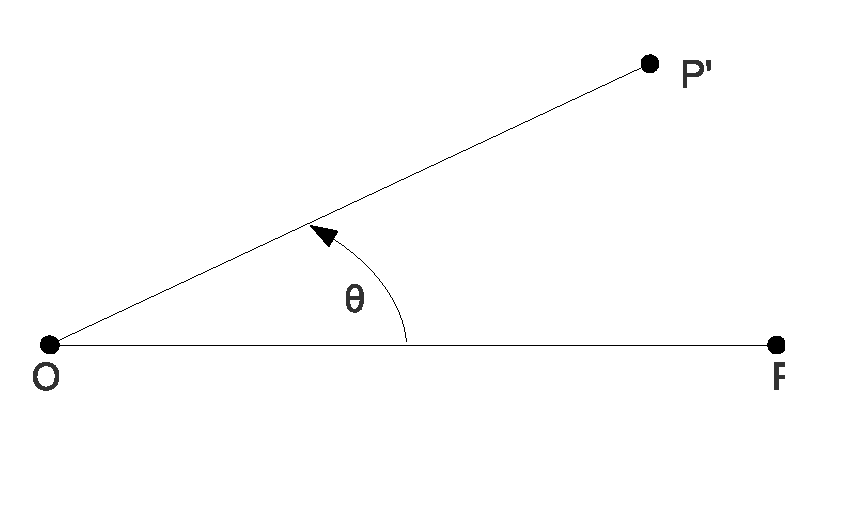
\includegraphics[width=5cm,keepaspectratio]{immagini/Capitolo_III/rotazione_piana}
		\centering
		\label{fig:rotpiana}
	\end {minipage}
	}
\end{figure}
dove \textbf{n} è il versore normale al piano nella direzione di rotazione positiva.

$\\$La rotazione nello spazio si può ricondurre a quella piana se si decompone il vettore posizione sul piano $\pi$ ortogonale all'asse di rotazione e passante per il punto P considerato.
$\\$Per la rotazione spaziale si trova che:
\begin{figure}[!h]
\centering
\mbox{%

	\begin{minipage}{.74\textwidth}
			\caption{Rotazione spaziale}	
	\begin{displaymath}
			\begin{array}{rcl}
			P_{*}P & = &  OP - OP_{*} = O - (OP\cdot \textbf{n})\textbf{n} \\
			PP' 	 & = & P_{*}P \cos(\theta) - P_{*}P + ( \textbf{n} \wedge \textbf{n}) \sin(\theta) = \\
 		        & = & (\cos(\theta)-1)( OP -(OP\textbf{n})\textbf{n}) +\sin(\theta)\textbf{n}\wedge OP \\
  			\end{array}
	\end{displaymath}				 
	\end {minipage}%
	
		\begin{minipage}{.50\textwidth}	
		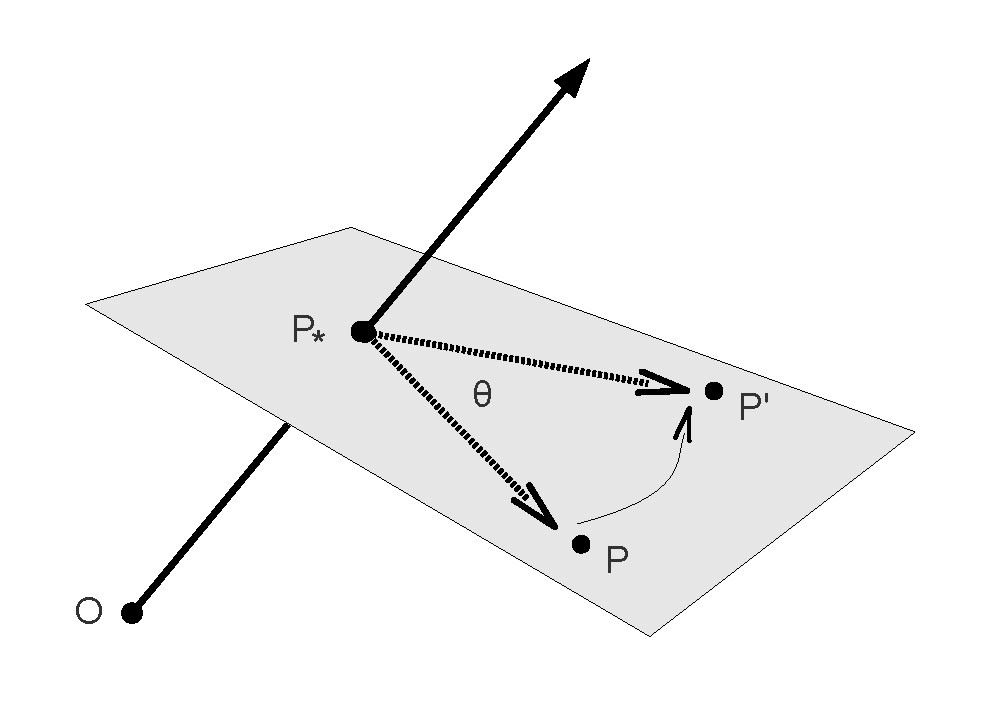
\includegraphics[width=6cm,keepaspectratio]{immagini/Capitolo_III/rotazione_spazio}
		\label{fig:rotspazio}
	\end {minipage}
	}

\end{figure}

quindi:
\begin{equation}\label{eq:rotazionespazio}
OP' = OP + PP' = (1 -\cos(\theta) )(OP\textbf{n})\textbf{n} + \cos(\theta)OP + \sin(\theta)\textbf{n}\wedge OP 
\end{equation}
$\\$
Da queste relazioni si ricava la dipendenza di $P'$ da $P$, punto che subisce la rotazione attiva, e dai  parametri che fissano la rotazione. 

$\\$
Pertanto si deduce che le rotazioni geometriche sono specificate univocamente dall'angolo di rotazione $\theta$ , dal versore dell'asse di rotazione \textbf{n} e dal punto di applicazione del versore (in altre parole dall'asse di rotazione).


Scelto un riferimento cartesiano, un versore è completamente determinato da 2 angoli, quindi l'insieme $(\theta,\alpha, \beta)$ costituisce le coordinate classiche associate alle rotazioni concorrenti nel punto O, ovvero tali che tutti i possibili assi hanno in comune l'origine del riferimento.

\subsection{Il Gruppo delle Rotazioni}

I risultati classici presentati nel paragrafo precedente possono essere riletti alla luce della teoria dei gruppi.


$\\$Per prima cosa bisogna notare che in geometria euclidea è implicita una legge di composizione gruppale per le isometrie (il discorso è valido anche per gli spostamenti rigidi), le isometrie si compongono tramite la loro applicazione consecutiva e la trasformazione risultate è ancora un'isometria. 
Le isometrie quindi costituiscono un gruppo caratterizzato dalla condizione che l'azione dei suoi elementi sullo spazio euclideo sia tale da matenere inalterata la distanza tra i punti. Trasalazioni e rotazioni sono delle particolari sottoclassi delle isometrie.
%di cui non è nota nello specifico l'azione sui punti dello spazio euclideo ma solo che devono soddisfare il vincolo di invarianza della distanza, trasalazioni e rotazioni sono particolari sottoclassi delle isometrie.

Si vuole a questo punto dimostrare che la classe delle rotazioni costituisca un sottogruppo delle isometrie, resta da verificare la chiusura. La chiusura delle rotazioni rispetto alla composizione è implicita nel \emph{II} teorema di Eulero: è chiaro che la composizione di due rotazioni con assi intersecati nel punto $O$ mantiene fissa tale punto, per il teorema tale trasformazione mantiene fiss almeno un altro punto, in altre parole, un asse rimane invariato.
Pertanto la composizione di due rotazioni concorrenti nel punto $O$ è ancora una rotazione dello stesso tipo con asse diverso dalle trasformazioni inziali (a meno che le rotazioni componenti non siano parallele).

É importante notare che la composizione di due rotazioni consecutive qualsiasi è ancora un'isometria ( \emph{Teorema di Chasles}) ma tale isometria è una rotazione solo nel caso che i due assi abbiano almeno un punto in comune, pertanto solo per le rotazioni conccorrenti in un punto si può individuare una legge di composizione gruppale.

Da questo è naturale rileggere la definizione di \emph{rotazione attiva}, dove semplicemente si identifica la rotazione come una funzione sullo spazio euclideo su se stesso, come l'espressione di un'azione di un particolare gruppo sullo spazio euclideo. 
Dalla definizione (\ref{def:azionegruppo}) l'azione del gruppo su $E^{3}$è una funzione $ \Phi : E^{3} \times G \rightarrow E $ tale che:
$$\Phi( P, R) = P' $$
con $P'$ specificato dall'equazione ( \ref{eq:rotazionespazio}).
Similmente l'azione sul piano $E^{2}$ è esplicitata dall'equazione (\ref{eq:rotazionepiano}).


Tale gruppo lo si può indentificare con il Gruppo delle Rotazioni \emph{Astratto}, indicato con $\mathscr{R}$.
Si dice \emph{Astratto} in quanto non è nota una rappresentazione esplicita degli elementi che lo compongono ma si è a conoscenza solo di una loro parametrizzazione e della azione determinata dal gruppo su alcune specifiche varietà. In questa definizione è sottointesa la scelta di un punto di orgine $O \in E^{3}$ comune agli assi di tutte le rotazioni appartenenti ad $\mathscr{R}$.

Una possibile parametrizzazione del gruppo $\mathscr{R}$ è quella classica, data da \textbf{n} versore dell'asse e $\theta$ angolo di rotazione, da cui si conclude che è un gruppo a 3 parametri.
\begin{oss}
Questa parametrizzazione non è univoca. Alle rotazioni specificate da $(\hat{n}, \theta)$ e $(-\hat{n}, -\theta)$ corrisponde lo stesso spostamento nello spazio Euclideo. In sintesi:
$$\Phi(P;\hat{n},\theta) = \Phi(P; -\hat{n}, -\theta) $$

\end{oss}

 Chiaramente quella appena definita non è l'unica  parametrizzazione possibile, è possibile individuare le altre realizzando degli isomorfismi tra il gruppo astratto e opportuni sottogruppi delle matrici o dei numeri ipercomplessi, il vantaggio di questo processo è la possibilità di dare una rappresentazione esplicita degli elementi che costituiscono il gruppo delle rotazioni astratto.
$\\$

Scopo del resto del capitolo sarà di analizzare qualche altro gruppo che "agisce" allo stesso modo di $\mathscr{R}$, in altre parole si cercheranno dei gruppi notevoli isomorfi al gruppo delle rotazioni astratto.

\section{Isomorfismo del gruppo delle rotazioni con SO(3)}

Guardando l'espressione analatica dello spostamento rotario (\ref{eq:rotazionespazio}) è evidente che l'azione del gruppo $\mathscr{R}$ su $E^{3}$ è lineare in $OP$, vettore associato al punto $P$.
Scegliendo un sistema di riferimento cartesiano nello spazio euclideo si possono identificare i punti di $E^{3}$ con i vettori di $\mathbb{R}^{3}$, pertanto ad ogni rotazione del gruppo $\mathscr{R}$ è possibile associare un'applicazione lineare su $\mathbb{R}^{3}$, in altre parole una matrice reale $3 \times 3$.

Da una semplice argomentazione dimensionale il gruppo $\mathscr{R}$( gruppo a 3 parametri) non potrà mai essere isomorfo a tutto $\textrm{GL}(n, \mathbb{R})$( gruppo a 9 parametri) al massimo potrà esserlo ad un suo sottogruppo.

Si può dimostrare che tale isomorfismo si realizza con il sottogruppo SO(3), un modo per vederlo è il seguente:
\begin{itemize}
	\item[-] Costruendo esplicitamente le matrici di rotazione rispetto agli assi del riferimento:

\begin{figure}[!h]
\mbox{%

		\begin{minipage}{.33\textwidth}	
		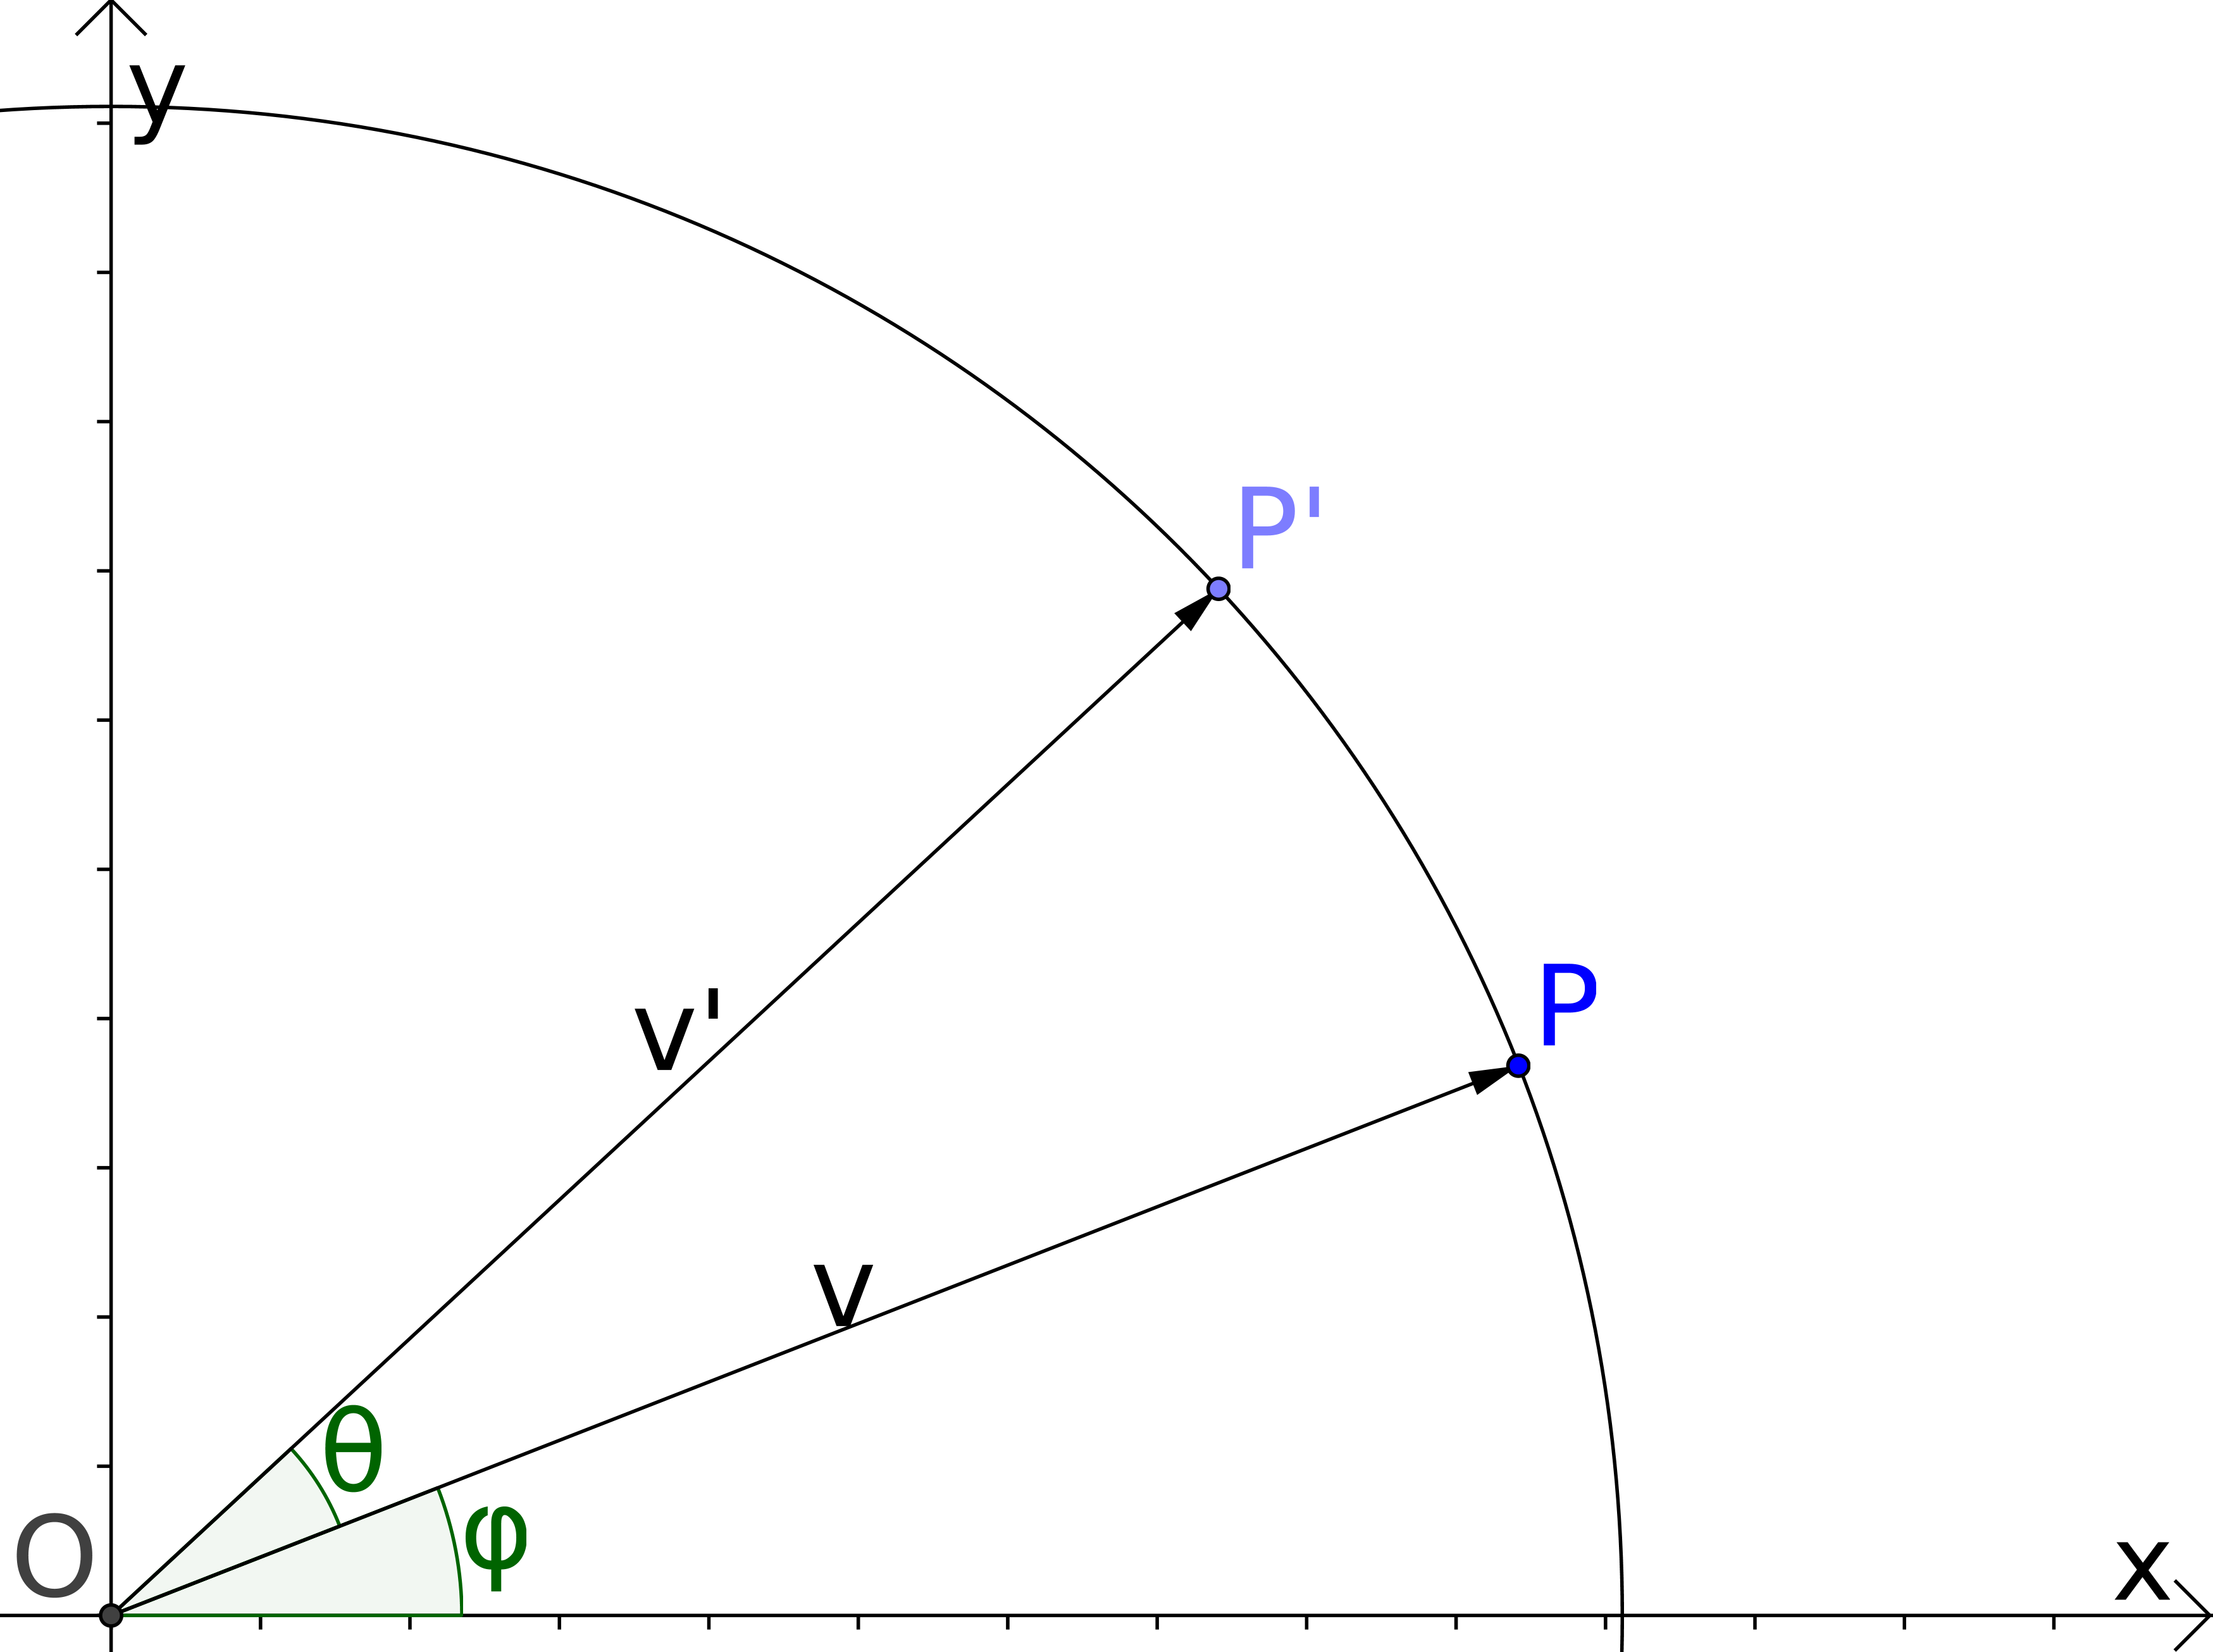
\includegraphics[width=5cm,keepaspectratio]{immagini/Capitolo_III/rotazioneelementare}
		\label{fig:rotattiva}
		\end {minipage}

	\begin{minipage}{.67\textwidth}
		\begin{displaymath}
	R_{z}(\theta) = \left[ \begin{array}{ccc}
\cos(\theta) & -\sin(\theta) & 0\\
\sin(\theta) & \cos(\theta) & 0\\
0 & 0 & 1 \\
\end{array} \right]
		\end{displaymath}		
	$\qquad$(le altre si ricavano in modo analogo) 
	\end {minipage}%
		}
\end{figure}


	
è evidente che in questi casi elementari le rotazioni sono rappresentate da matrici ortogonali speciali.
	\item[-] A questo punto bisogna dimostrare che ogni rotazione appartiene a  SO(3). Per farlo bisogna dimostare come sia possibile costruire ogni generica rotazione di asse \textbf{n} e angolo $\theta$ come composizione di rotazioni rispetto agli assi fissi. Il procedimento è semplice, prima si effettuano due rotazioni consecutive per sovrapporre l'asse di rotazione \textbf{n} con l'asse $z$ del sistema di riferimento, a questo punto si applica la rotazione dell'angolo desiderato $\theta$ attorno all'asse $z$ e infine si applica l'inverso della trasformazione iniziale in modo da riportare l'asse \textbf{n} nella sua posizione iniziale; in totale la generica rotazione risulta la composizione di cinque rotazioni rispetto assi fissi.
	
\begin{figure}[!h]
\mbox{%

		\begin{minipage}{.38\textwidth}	
		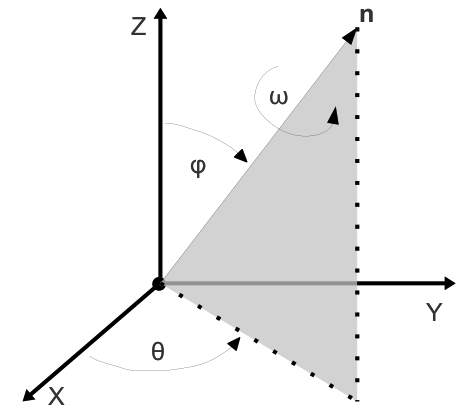
\includegraphics[width=7cm,keepaspectratio]{immagini/Capitolo_III/rotazioneattiva.jpg}
		\label{fig:rotattiva}
		\end {minipage}

	\begin{minipage}{.74\textwidth}
			\caption{Generica Rotazione}	
	\begin{equation}
	R_{\textbf{n}}(\omega) =R_{z}(\theta)R_{y}(\phi)R_{z}(\omega)R_{y}(-\phi)R_{z}(-\theta) 
	\end{equation}				 
	\end {minipage}%
		}
\end{figure}

Per la proprietà gruppale la matrice $R_{\textbf{n}}(\omega) $ associata alla generica rotazione è anch'essa un elemento di SO(3).

\end{itemize}

In conclusione questo isomorfismo permette di associare ad ogni elemento di $\mathscr{R}$  una matrice, quindi è possibile parametrizzare il gruppo tramite le sue componenti, detti in questo caso \emph{coseni direttori}.
Da  un punto di vista più astratto si potrebbe dire che il procedimento precedento ha portato ad individuare un sottogruppo di matrici $3 \times 3$ la cui azione su $E^{3}$ è identica a quella delle rotazioni astratte, questo giustifica l'identificazione 1:1 (isomorfismo) di $\mathscr{R}$ con $SO(3)$, entrambi gruppi a 3 parametri.

$\\$
In altre parole $SO(3)$ è la \emph{Rappresentazione}, nel senso chiarito dalla definizione (\ref{def:azionegruppo}) del gruppo $\mathscr{R}$ su $E^{3}$.


\section{Omomorfismo tra il gruppo delle rotazioni e  SU(2)}

Per mostrare la corrispondenza tra il gruppo delle rotazioni e il gruppo SU(2) bisogna partire un'altra volta dall'azione del gruppo delle rotazioni sullo spazio euclideo; fissando un'origine $O \in E^{3}$ e associando al generico punto $P$ il vettore $\textbf{r}=\vec{OP}$, l'equazione dell'azione assume la forma:

\begin{equation}\label{eq:rotazionevettori}
\Phi(\textbf{r}; \theta, \hat{n}) = \bar{\textbf{r}} = (1-\cos(\theta))(\textbf{r}\cdot\textbf{n})\textbf{n} + \cos(\theta)\textbf{r} +\sin(\theta)(\textbf{n}\wedge\textbf{r})
\end{equation}
se $\textbf{n}$ coincide con l'asse $z$ si ritrova l'usuale rotazione nel piano (eq:\ref{eq:rotazionepiano}) ovvero:
	\begin{displaymath}
			\begin{array}{c}
 			\bar{x_{1}} = \cos(\theta) x_{1} - \sin(\theta) x_{2}\\	
 			\bar{x_{2}} = \sin(\theta) x_{1} + \cos(\theta) x_{2}\\
  			\bar{x_{3}} = x_{3}\\
  			\end{array}
	\end{displaymath}
	
$\\$La rotazione nel piano ammette una comoda rappresentazione complessa. Associando ad ogni punto del piano il numero complesso $z= x_{1}+ix_{2}$ si trova che:

	\begin{displaymath}\begin{split}
			e^{i\theta}z &= (\cos(\theta)+i\sin(\theta))(x_{1}+ix_{2})=(\cos(\theta)x_{1}-\sin(\theta)x_{2}) + i(\sin(\theta)x_{1}+\cos(\theta)x_{2})\\ &=\bar{x_{1}} + i\bar{x_{2}}=\bar{z}
	\end{split}\end{displaymath}
La precedente equazione può essere vista come l'azione del sottogruppo delle rotazioni piane su $\mathbb{C}$:
$$\phi: \mathbb{C} \times \mathscr{R_{z}} \qquad \phi( z, \theta) = e^{i\theta}z$$
dove $\mathscr{R_{z}}$ è il sottogruppo formato dalle rotazioni con asse fisso $z$.

In altre parole le rotazioni piane ammettono una rappresentazine tramite numeri complessi di modulo unitario ($\mathbb{C}$ in quanto \emph{campo} soddisfa naturalmente la definizione di gruppo rispetto al prodotto di numeri complessi).$\\$

Alla luce di ciò si intende estendere questo approccio alle più generali rotazioni spaziali del gruppo $\mathscr{R}$, la difficoltà sta nelle dimensioni.
Mentre il gruppo delle rotazioni piane è specificato da un solo parametro (l'angolo di rotazione $\theta$), le generiche rotazioni ne richiedono tre, sarà quindi necessario introdurre una generalizzazione dei numeri complessi di norma 1: i \emph{numeri ipercomplessi}.

\subsection{Rappresentazione quaternionale delle rotazioni}
In generale si definisce un numero ipercomplesso come un oggetto nella forma 
$$\mathsf{q} = a_{0} + a_{i}e_{i} \qquad \textrm{con} \;a_{0},a_{i} \in \mathbb{R}$$
dove gli elementi $e_{i}$ costituiscono la generalizzazione dell'unità immaginaria $i$.

$\\$ Nello specifico si definisce:
\begin{defn}[\textbf{Quaternione}]\label{def:quaternione}$\\$
Numero ipercomplesso a 4 componenti $\mathsf{a} = a_{0} + a_{i}e_{i}$ con $a_{0},a_{i} \in \mathbb{R}$ e $e_{i}\in\{ 1,2,3\}$ tale che:
	\begin{displaymath}
	e_{i}e_{j} = \left\{ 
			\begin{array}{l c c}
 			e_{i}^{2}=-1 & & i=j=1,2,3\\	
 			e_{i}e_{j}= \epsilon_{ijk} e_{k} & & i \neq j \\
  			\end{array} \right.
	\end{displaymath}	
\end{defn} 

Sui quaternioni, similmente ai numeri complessi, sono definite le operazioni:
\begin{itemize}
	\item[-]\emph{Somma} $$\mathsf{p} + \mathsf{q} = p_{0} + p_{i}e_{i} + q_{0} + q_{i}e_{i} = (p_{0} + q_{0}) +(p_{i} + q_{i})e_{i} = \mathsf{s} $$
	\item[-]\emph{Prodotto} $$\mathsf{p}\mathsf{q} = (p_{0} + p_{i}e_{i} )( q_{0} + q_{i}e_{i}) = p_{0}q_{0} + (p_{0}q_{i} + q_{0}p_{i})e_{i} - p_{i}q_{i} + p_{i}q_{i}e_{k}\epsilon_{ijk} $$
	\item[-]\emph{Coniugio} $$\mathsf{q}^{*} = q_{0} - q_{i}e_{i} $$
	\item[-]\emph{Norma} $$\mid\mathsf{q}\mid = \mathsf{q}^{*}\mathsf{q} = \mathsf{q}\mathsf{q}^{*}=q_{0}^{2}  + q_{i}q_{i}$$
\end{itemize}

La presenza del prodotto fa si che l'insieme $\mathbb{H}$ dei quaternioni costituisca un gruppo non commutativo; più precisamente si tratta di un corpo( non commutativo): soddisfa quindi tutte le proprietà usuali dei campi, quali i numeri reali o complessi, tranne la proprietà commutativa del prodotto.

I quaternioni contengono i numeri complessi, e sono anche uno spazio vettoriale sui numeri reali a 4 dimensioni (analogamente ai complessi, che sono uno spazio sui reali a 2 dimensioni).

%Il numero delle componenti del quaternione giustifica l'introduzione di una comoda notazione vettoriale:
%$$\mathsf{q}= q_{0} + \vec{q} = q_{0} + q_{1}\vec{\mu} $$
%dove $q_{0}$ e $q_{1} \in \vec{R}$ e $\vec{\mu}$ è un versore a tre componenti di norma unitaria. 

%Il prodotto tra quaternioni si può leggere come:
%$$\mathsf{p}\mathsf{q} = p_{0}q_{0} - \vec{p}\vec{q} + p_{0}\vec{q} + q_{0}\vec{p} + \vec{p}\wedge \vec{q}$$

%E la norma come:
%$$\mathsf{q}^{*}\mathsf{q} = (q_{0} + q_{1}\vec{\mu})(q_{0} - q_{1}\vec{\mu}) = q_{0}^{2} -\vec{\mu}\cdot\vec{\mu}q_{1}^{2}= q_{0}^{2} + q_{1}^{2} $$

%pertanto il prodotto di $\vec{\mu}$ con se stesso va inteso in senso quaternionale, deve valere quindi che$\vec{\mu}\cdot\vec{\mu}=-1$ in altre parole $\vec{\mu}$ è l'analogo dell'unità immaginaria $i$.

%Questa notazione apre anche la possibilità di associare ad ogni vettore di $\vec{r} \in \mathbb{R}^{3}$ un quaternione $\mathsf{r}= 0 +\vec{r}$ di parte scalare nulla, da questo emerge naturalmente un legame con il gruppo delle rotazioni $\mathscr{R}$.
$\\$

Definendo il quaternione di rotazione come:
\begin{equation}\label{eq:rotquaternio}
\mathsf{q}_{\mathscr{R}} = \cos(\frac{\theta}{2}) + \sin(\frac{\theta}{2})\hat{n}
\end{equation}
e  associando ad ogni vettore di $\vec{r} \in \mathbb{R}^{3}$ un quaternione $\mathsf{r}= 0 +x_{i} e_{i}$ di parte scalare nulla ( elemento di $\mathbb{H}_{imm}$) , si ottiene, sfruttando le formule di duplicazione degli angoli, l'equazione:
\begin{equation}\label{eq:azionequaternioni}
\mathsf{q}\mathsf{r}\mathsf{q}^{*} = 0 + \cos(\theta)\vec{r} + (1 -\cos(\theta))(\vec{r}\cdot \hat{n})\hat{n} + \sin(\theta) \hat{n}\wedge\vec{r} = \bar{\mathsf{r}}
\end{equation}
che coincide con l'equazione (\ref{eq:rotazionevettori}).

Quindi se $\mathsf{r}$ è il quaternione associato al vettore posizione del punto $P$ si trova che $\bar{\mathsf{r}}$ è il quaternione relativo alla posizione del punto ottenuto ruotanto $P$ di un angolo $\theta$ rispetto alla direzione $\hat{n}$.

$\\$Pertanto l'equazione (\ref{eq:azionequaternioni}) rappresenta un'azione $\phi: \mathbb{H}_{imm} \times \mathscr{R} \rightarrow \mathbb{H}_{immt} $ del gruppo delle rotazioni sullo spazio $\mathbb{H}_{imm} \simeq \mathbb{R}^{3} $ dei quaternioni vettoriali puri tale che $$\phi( \mathsf{r} ; \hat{n}, \theta) = \mathsf{q}\mathsf{r}\mathsf{q}^{*}$$

L'equazione (\ref{eq:rotquaternio}) è l'espressione più generale per i quaternioni di norma uno e naturalmente i quaternioni unitari formano un sottogruppo di $\mathbb{H}$.
Una volta verificato che la composizione di due rotazioni di quaternioni, nel senso espresso dall'equazione (\ref{eq:azionequaternioni}) (basta verificare che $(\mathsf{q}\mathsf{p})^{*} = \mathsf{p}^{*}\mathsf{q}^{*}$), è ancora una rotazione, si può concludere che il gruppo dei quaternioni unitari è omomorfo al gruppo $\mathscr{R}$

\begin{oss}$\\$
In questo caso non si può parlare di isomorfismo, ma bensì di omomorfismo, in quanto fra il gruppo $\mathscr{R}$ e il sottogruppo $\mathbb{H}_{unit}$ dei quaternioni unitari vi è una corrispondenza uno a due. Infatti dall'equazione (\ref{eq:azionequaternioni}) si nota che se $\mathsf{q} $ è un quaternione unitario sia $\mathsf{q} $  che $- \mathsf{q} $ rappresentano la stessa rotazione.
In altre parole $\mathbb{H}_{unit}$ costituisce un doppio ricoprimento di $SO(3)$.
\end{oss} 
\begin{figure}[!h]

		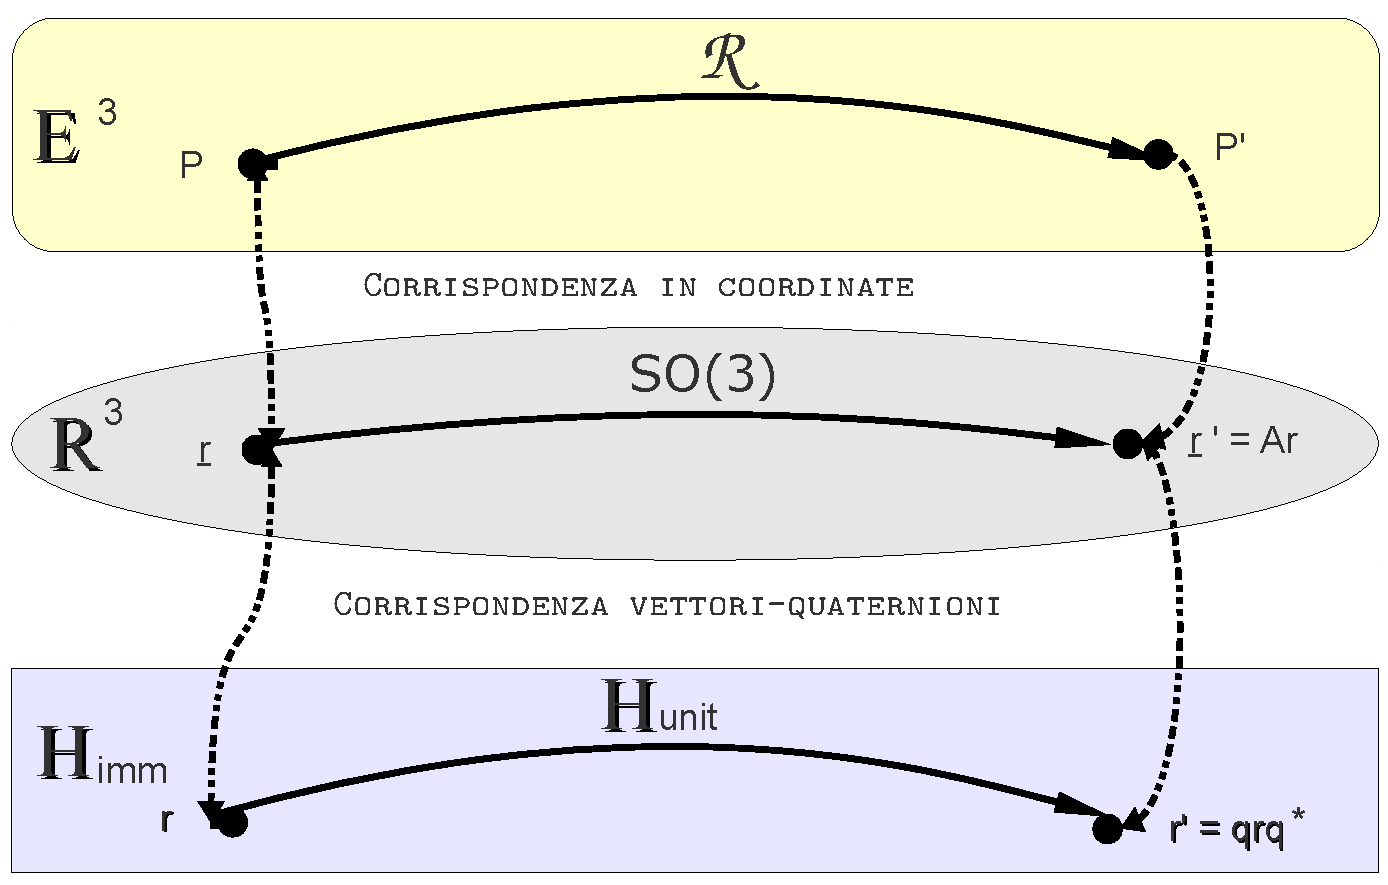
\includegraphics[width=15cm,keepaspectratio]{immagini/Capitolo_III/schemaisomorfismi}
		\label{fig:schemaisometrie}
			\caption{Schema riassuntivo degli isomorfismi}					 
\end{figure}
La corrispondenza tra rotazioni e quaternioni permette di introdurre una nuova parametrizzazione del gruppo $\mathscr{R}$, si può specificare la generica rotazione tramite le coordinate del quaternione ad essa associato .
Ad una rotazione di angolo $\theta$ e versore \textbf{n} si associeranno 4 numeri reali $(q_{0},q_{1},q_{2},q_{3})$ detti \emph{parametri di Eulero} tali che:
	\begin{displaymath}
\left\{ 
			\begin{array}{c c c}
 			q_{0} & = & \cos(\frac{\theta}{2})  \\	
 			q_{0} & = & \sin(\frac{\theta}{2})\cos(\alpha) \\
 			q_{0} & = & \sin(\frac{\theta}{2})\cos(\beta) \\
 			q_{0} & = & \sin(\frac{\theta}{2})\cos(\gamma) \\  			\end{array} \right.
	\end{displaymath}	
dove $(\alpha, \beta, \gamma)$ sono i coseni direttori dell'asse di rotazione.
 
\subsection{Isomorfismo dei quaternioni unitari con SU(2)}
É possibile realizzare un isomorfismo tra lo spazio $H$ dei quaternioni e le matrici $2 \times 2$, sia $\mathsf{a} = a_{0} + a_{i}e_{i}$ un generico quaternione, definendo $\sigma_{j} = i e_{j} $ tale quaternione può essere scritto come:
$$\mathsf{a} = a_{0} - i a_{k}\sigma_{k}$$

$\\$Dalla definizione (\ref{def:quaternione}) risultà che le quantita $\sigma_{k}$ soddisfano le seguementi proprietà: 
	\begin{equation}\label{eq:algebrapauli}
	\left\{ 
			\begin{array}{l c c}
 			\sigma_{k}^{2}=-e_{k}^{2}=1 & & \\	
 			\sigma_{k}\sigma_{l}=-e_{k}e_{l}=- \epsilon_{klm} e_{m} = i\epsilon_{klm} \sigma_{k}  & & k \neq l \\
  			\end{array} \right.
	\end{equation}	
che coincidono con le regole di commutazione delle matrici di Pauli:

\begin{figure}[!h]
\mbox{%

	\begin{minipage}{.33\textwidth}	
\begin{displaymath}
\sigma_{1} = \left[ \begin{array}{cc}
0 & 1  \\
1 & 0  \\
\end{array} \right]
\end{displaymath}	
	\end {minipage}

	\begin{minipage}{.33\textwidth}	
\begin{displaymath}
\sigma_{2} = \left[ \begin{array}{cc}
0 & -i  \\
i & 0  \\
\end{array} \right]
\end{displaymath}	
\end {minipage}

	\begin{minipage}{.33\textwidth}	
\begin{displaymath}
\sigma_{3} = \left[ \begin{array}{cc}
1 & 0  \\
0 & -1  \\
\end{array} \right]
\end{displaymath}	
\end {minipage}%
		}
\end{figure}
In altre parole le matrici di Pauli rappresentano il gruppo finito costituito dai 3 elementi $\sigma_i$ e di cui il sistema (\ref{eq:algebrapauli}) esaurisce in modo completo la descrizione delle regole di composizione gruppale.

$\\$In virtù di questo, il generico quaternione ammette la seguente notazione matriciale
\begin{equation}
\mathsf{q} =  q_{0}\mathbb{I} -i q_{k}\sigma_{k} = \left[ \begin{array}{cc}
q_{0}- i q_{3} & -iq_{1}-q_{2}  \\
-q_{1} + q_{2} & q_{0}+iq_{3}  \\
\end{array} \right] = \left[ \begin{array}{cc}
\alpha & \beta  \\
-\beta^{*} & \alpha^{*}  \\
\end{array} \right] = U
\end{equation}
Riducendosi ai soli quaternioni unitari si trova che la matrice associata soddisfa le seguenti proprietà:
\begin{itemize}
\item[-] ha determinante 1 $$det(U) = \alpha \alpha^{*} + \beta \beta^{\*} = q_{0}^{2} + q_{1}^{2} + q_{2}^{2} + q_{3}^{2} = \mathsf{q} \mathsf{q}^{*} = 1$$
\item[-] è unitaria 
\begin{displaymath}
U U^{\dagger} = 
\left[ \begin{array}{cc}
\alpha & \beta  \\
-\beta^{*} & \alpha^{*}  \\
\end{array} \right] 
\left[ \begin{array}{cc}
\alpha^{*} & -\beta  \\
\beta^{*} & \alpha  \\
\end{array} \right] =
\left[ \begin{array}{cc}
\alpha^{2} + \beta^{2} & 0  \\
0 & \alpha^{2} + \beta^{2}  \\
\end{array} \right] = U^{\dagger} U = Id
\end{displaymath}
\end{itemize}
pertanto si può concludere che il gruppo $SU(2)$ delle matrici unitarie speciali a coefficienti complessi è isomorfo al gruppo dei quaternioni unitari $\mathbb{H}_{unit}$ che a sua volta è omomorfo al gruppo $\mathscr{R}$ delle rotazioni astratte e quindi a $SO(3)$.

I coefficienti $\alpha, \beta \in \mathbb{C}$ nel caso di matrici di rotazione sono detti parametri di Cayley-Klein, costituiscono una parametrizzazione del gruppo quaternioni unitari quindi, di conseguenza, del gruppo delle rotazioni.
\begin{displaymath}
 \begin{array}{ccccc}
\alpha & = & q_{0} - i q_{3} & = & \cos(\frac{\theta}{2}) - i \sin(\frac{\theta}{2})\cos(\gamma)  \\
\beta & = & -i q_{1} - q_{2} & = & \sin(\frac{\theta}{2})\cos(\alpha) + \sin(\frac{\theta}{2})\cos(\beta)\\
\textrm{Cayley-Klein} & & \textrm{Eulero} & & \textrm{rotazione classica}
\end{array} 
\end{displaymath}




\section{Azione del gruppo delle rotazioni sui Riferimenti (rotazioni passive)}

Fin ora si è parlato delle rotazioni come delle \emph{azioni} su $ E^{3} \simeq \mathbb{R}^{3}$ , quindi come delle funzioni che mandano un punto dello spazio euclideo in un altro punto, per questo sono state chiamate "attive" oppure "spostamenti rotatori" nel linguaggio delle meccanica.

Scegliendo un riferimento cartesiano sullo spazio, associando quindi ad ogni punto il vettore delle coordinate,  il gruppo delle rotazioni può essere rappresentato dal gruppo SO(3), la sua azione su un punto $P$ coincide con l'applicazione di una matrice ortogonale speciale al vettore delle coordinate.

Nulla vieta però di leggere l'azione di una matrice ortogonale speciale sullo spazio $\mathbb{R}$ come un'applicazione che altera le coordinate del punto senza però spostarlo, in altre parole come un cambio di sistema di coordinate.

\begin{displaymath}
\begin{array}{ccccc}
 &  & E^{3} &  & \\
 & &\downarrow & ^{\textrm{scelta di un riferimento}}&\\
 \mathbb{R}^{3} &  \xleftarrow[\textrm{  cambio di riferimento  }]{S0(3)} & \mathbb{R}^{3} & \xrightarrow[\textrm{ rotazione attiva }]{S0(3)} & \mathbb{R}^{3}\\

\end{array}
\end{displaymath}


Risulta infatti che anche la generica applicazione di cambio di riferimento cartesiano che non altera l'origine degli assi è anch'essa rappresentata da una matrice ortogonale speciale. Il motivo è semplice: una qualsiasi trasformazione di questo tipo si riduce banalmente ad un endomorfismo sullo spazio delle coordinate, vettoriale e di dimensione finita, la cui rappresentazione matriciale avrà come righe le coordinate dei vettori della nuova base rispetto alla vecchia base in quanto:
\begin{equation}\label{eq:azionedestrariferimenti}
\begin{array}{|c|}
 \bar{\mathbf{e_{1}}} \\
 \bar{\mathbf{e_{2}}}\\
 \bar{\mathbf{e_{3}}}\\
\end{array} = A \cdot \begin{array}{|c|}
 \mathbf{e_{1}} \\
 \mathbf{e_{2}}\\
 \mathbf{e_{3}}\\
\end{array}
\end{equation}
dove $A$ è la matrice che rappresenta il cambiamento di base.
Ma i riferimenti cartesiani sono caratterizzati da un sistema di versori ortonormati, pertanto $A$ appartiene necessariamente ad $SO(3)$.

Si può parlare in questo caso di \emph{rotazioni passive} come il gruppo astratto la cui azione sullo spazio dei riferimenti $F_{(E^{3})}$ manda sistemi di cordinate cartesiane in sistemi di coordinate cartesiane, a livello astratto si tratta di un gruppo diverso da quello delle rotazioni attive ma siccome entrambi i gruppi sono isomorfi al gruppo $SO(3)$ si conclude che sono isomorfi tra loro. 

\begin{figure}[!h]	\label{fig:confrontorotazioni}
\centering
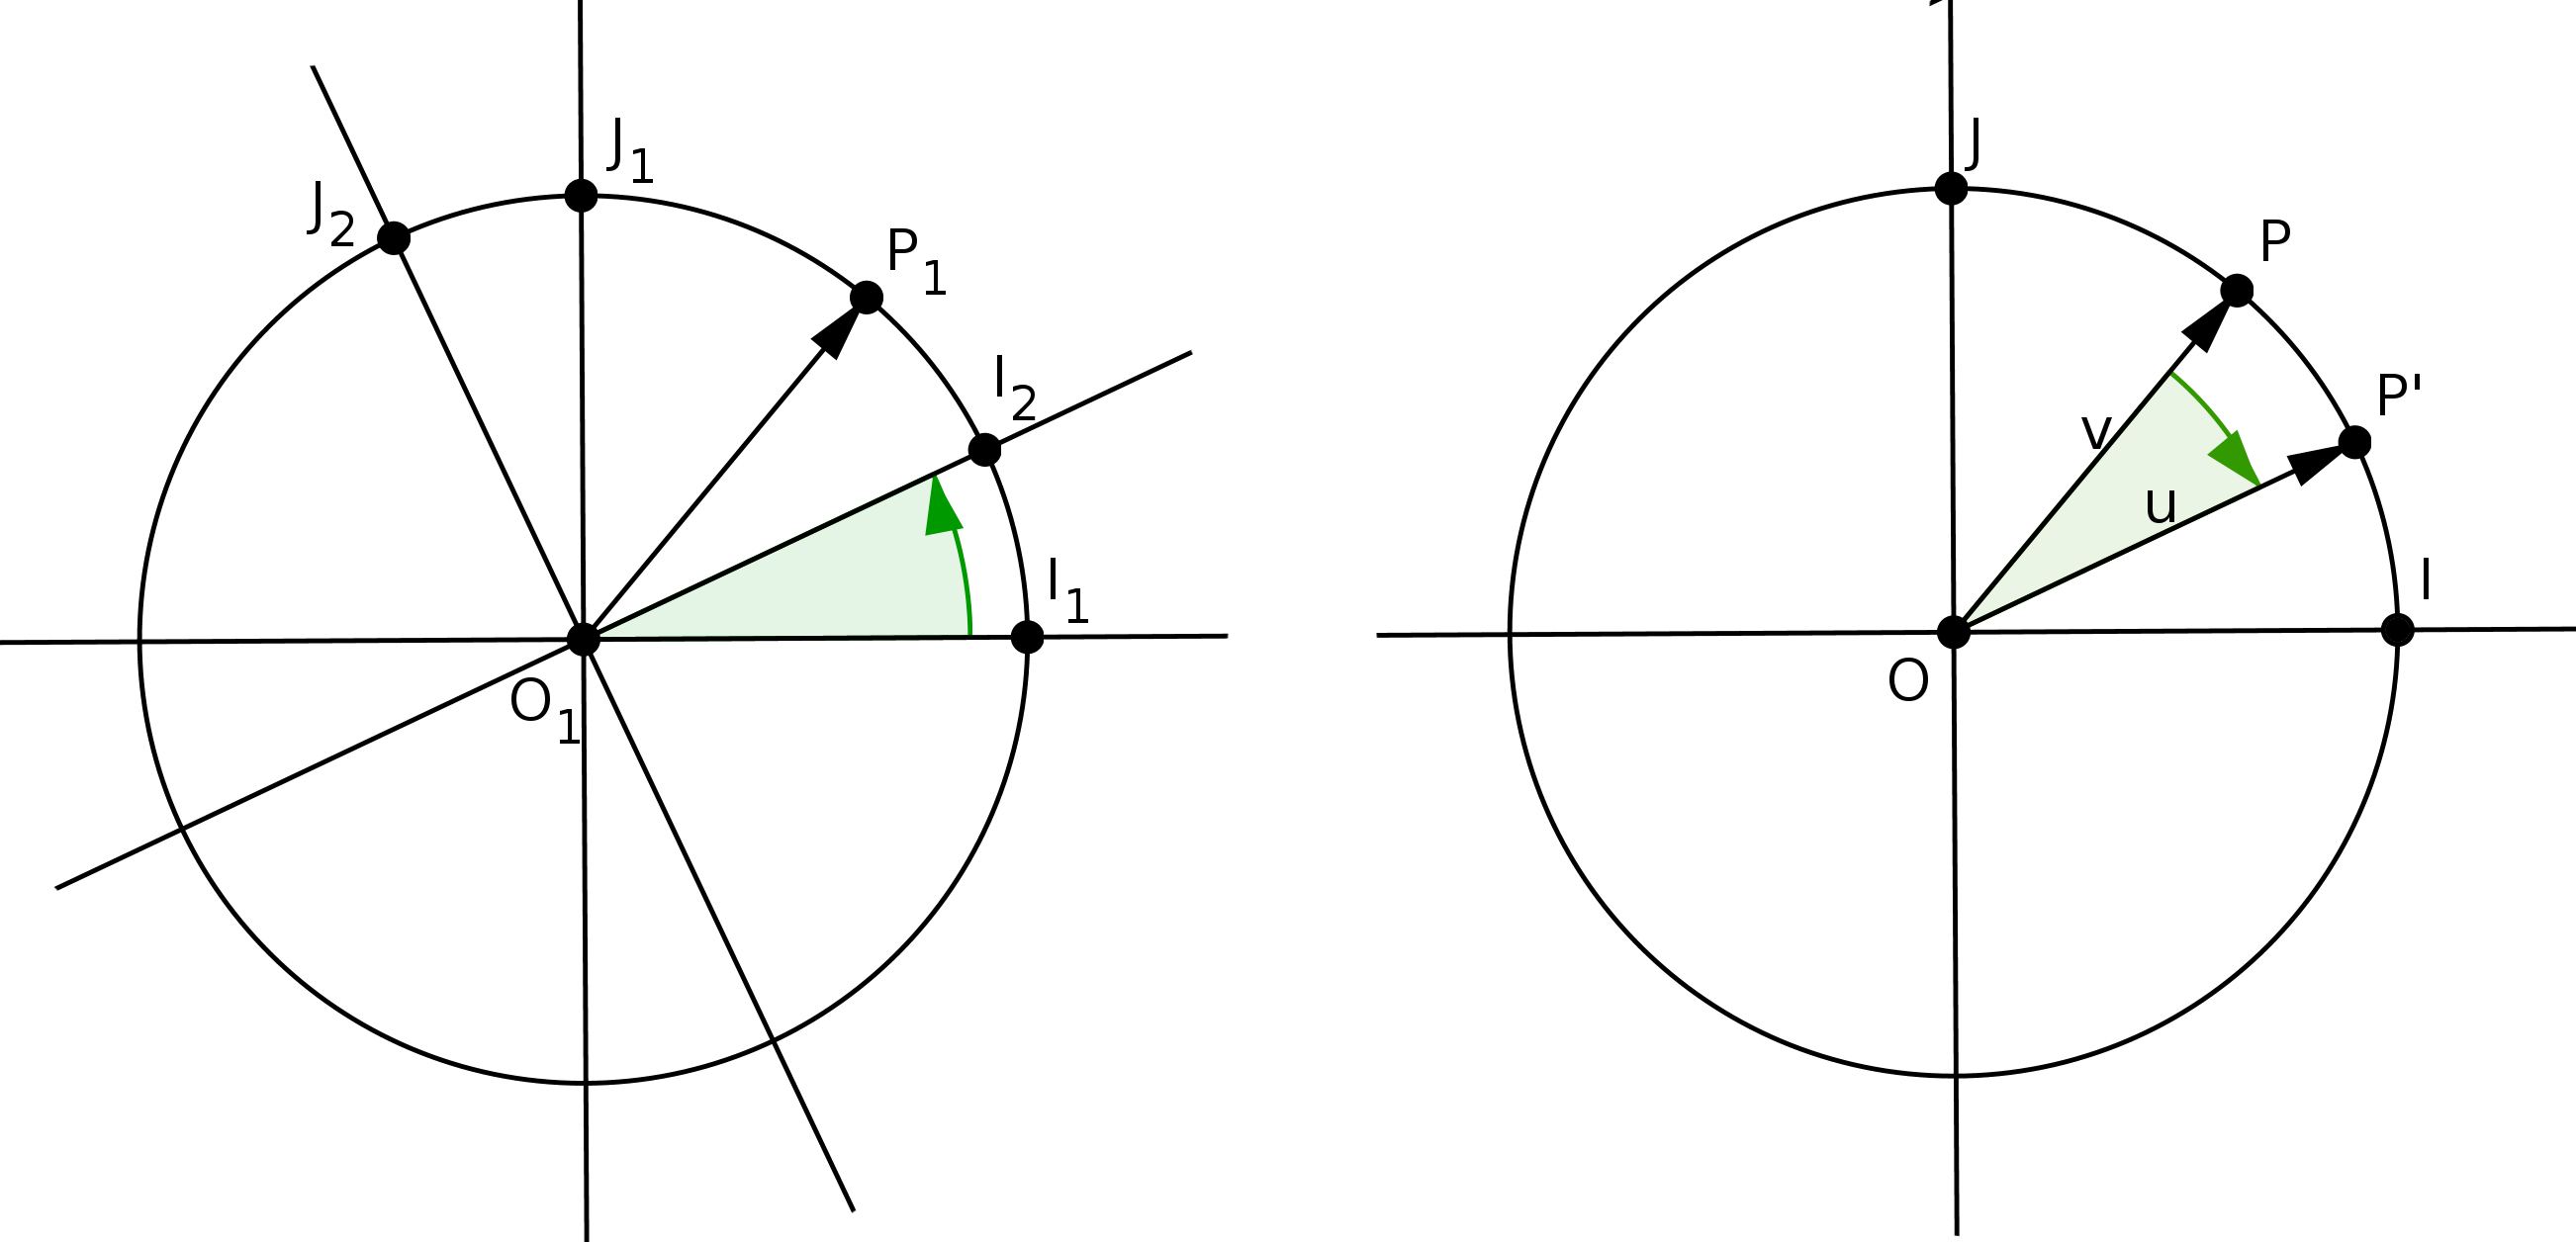
\includegraphics[width=12cm,keepaspectratio]{immagini/Capitolo_III/rotazioniattivepassive}	
\caption{Confronto rotazione attiva e passiva}
\end{figure}

L'isomorfismo si realizza notando che l'applicazione di una rotazione attiva di angolo $\theta$ attorno all'asse \textbf{n} ad un punto $P$ cambia le coordinate del punto allo stesso modo di una rotazione passiva di stesso asse ma di angolo opposto (figura [\ref{fig:confrontorotazioni}]).

Si può dire in alternativa che c'è un solo gruppo astratto, questo agisce sullo spazio $\mathbb{R}^{3}$ delle coordinate dei punti dello spazio euclideo come $A x = x'$ mentre agisce sullo spazio $F_{E^{3}}^{\bot}$ dei riferimenti cartesiani sullo spazio euclideo come $ \mathbb{e'} = A^{T}\mathbb{e'} $ dove $\mathbb{e}$ e $\mathbb{e}'$ rappresentano i riferimenti, sono dei vettori che hanno per componentii versori del sistema di riferimento.

\subsection{Parametrizzazione delle rotazioni tramite gli angoli di Eulero}
Sulle rotazioni dei sistemi di riferimento si può intrudurre la notazione degli angoli di Eulero che per l'isomorfismo si trasferisce naturalmente al gruppo delle rotazioni in generale.
La generica rotazione passiva, intesa come cambio di riferimento cartesiano che tiene fisso l'origine, si può ottenere componendo 3 rotazioni consecutive rispetto ad assi semplici:

\begin{equation}
(x,y,z)\xrightarrow{R^{ex}_{z}(\phi) \cdot R^{ex}_{x}(\theta)\cdot R^{ex}_{z}(\psi)} (x',y',z')
\end{equation}
bisogna osservare che la seconda rotazione $R^{ex}_{x}(\theta)$ non agisce sull'asse $z$ specificato dalla terna iniziale ma agisce sull'asse z del nuovo riferimento $R^{ex}_{z}(\psi) \cdot (x,y,z)^{T} $ come specificato dall'equazione (\ref{eq:azionedestrariferimenti}).


\begin{figure}[!h]\label{fig:euler}
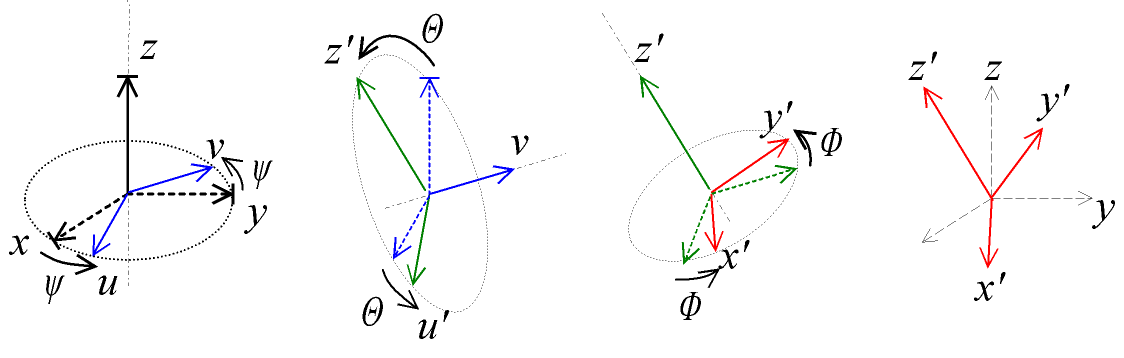
\includegraphics[width=15cm,keepaspectratio]{immagini/Capitolo_III/EulerG}			
			\caption{Angoli di Eulero}
\end{figure}

La maggiore semplicità di decomposizione di una rotazione in questi parametri si paga con una complicata legge di conversione tra gli angoli di eulero e i parametri di rotazione classica.

\subsection{Lo spazio di configurazione del corpo rigido}

Lo studio dell'azione di $\mathscr{R}$ sullo spazio dei riferimenti cartesiani è un buon punto di partenza per dimostrate come lo spazio di configurazione $Q$ del corpo rigido con  punto fisso si identifichi con il gruppo delle rotazoni quindi con $SO(3)$.
$\\$
Un corpo rigido è definito in meccanica come un sistema di almeno tre punti materiali non allineati tale per cui la distanza reciproca tra tutte le "particelle" che lo compongono rimane costante durante il moto o,in altre parole, è preservata in ogni spostamento del sistema.

$\\$
Si consideri ora un sistema cartesiano solidale con il corpo e formato dai 3 assi ortogonali $(i , j , k)$ e dal punto $O$. Solidale implica che le coordinate di ogni punto $P \in \Omega$ (dominio dello spazio euclideo occupato dal corpo) rispetto a questo riferimento rimangono invariate durante il moto. Il vincolo di rigidità tra i punti si rilegge quindi come un vincolo di rigidità tra ogni punto e il riferimento, pertanto è possibile identificare completamente le configurazioni del corpo con le configurazione del riferimento e il moto del corpo con il moto di una terna di assi ortonormali nello spazio.

$\\$
Se , a questo punto, si sceglie un secondo sistema di assi cartesiani $(I, J, K)$ fissi nello spazio, che si assume coincidere con la configurazione del sistema solidale in un istante $t_{0}$, è possibile descrivere la configurazione del corpo dopo uno spostamento arbitrario dando la trasformazione che manda la configurazione di riferimento $(I, J, K)$ nella generica configurazione $(i,j,k)$.

$\\$
Nel caso del corpo rigido con punto fisso, identificato ormai con i riferimenti cartesiani, queste trasformazioni non sono altro che  le matrici $SO(3)$.
$\\$
Pertanto $SO(3)$ coincide con $Q$ ma è ancora valido quanto detto prima, $SO(3)$ è anche l'azione di $\mathscr{R}$ su questo gruppo.
Secondo il formalismo sviluppato nei precedenti capitoli l'azione di questo gruppo su se stesso, quindi quella del gruppo delle rotazioni su $Q$, è data dalla traslazioni del gruppo $SO(3)$ nel senso chiarito dalle definizioni (\ref{def:traslsinistra} ) e (\ref{def:trasldestra}).

$\\$
\begin{oss}$\\$
Questa filosofia di parametrizzazione dei sistemi si può estendere anche a casi più generali.
% [fare riferimento a holm capitolo 11].

Si consideri ad esempio un fluido continuo di particelle materiali  , si battezza $\Omega \subset E$ il dominio occupato da questo sistema nel istante $t_{0}$.
Si prenda come configurazione di riferimento lo stato del sistema nell'istante $t_{0}$, è possibile parametrizzare le particelle costituente il corpo con la n-pla di coordinate $x \in \mathbb{R}$, detta etichetta, di ogni punto $P \in \Omega$ rispetto ad un prescelto sistema di coordinate in $E$.

A questo punto, la generica configurazione di questo sistema, non è altro che un elemento di $\textrm{Diff}(D)$, spazio dei diffeomorfismi di $D$ in se stesso, i cui elementi mandano il generico punto $X(t_{0})$ in un'altro punto $X(t)$ della sua traiettoria.
I diffeomorfismi chiaramente costituiscono un gruppo rispetto alla normale composizione di funzioni, la difficoltà di questo approccio è nel fatto che tale gruppo è infinito dimensionale. 
\end{oss}





\clearpage
\chapter{Struttura geometrica del gruppo delle rotazioni}
Dal capitolo precedente è evidente la moltitudine di punti di vista da cui si può affrontare lo studio delle rotazioni, lo studio ha portato ad identificare un solo gruppo astratto di cui ,ad esempio, le rotazioni attive o passive non sono altro che l'azione di questo gruppo su varietà differenti.

Inoltre si è dimostrato che il gruppo $\mathscr{R}$ è isomorfo al gruppo di Lie delle matrice ortogonali speciali, nulla vieta a questo punto di identificare direttamente le rotazioni con SO(3). Questo processo ha il vantaggio di fornire una rappresentazione esplicita degli elementi del gruppo, pertanto apre la possibilità di realizzare direttamente le strutture gruppali presentate nei primi due capitoli.

\section{Struttura differenziale di SO(3)}

Innanzi tutto si analizzano le strutture di SO(3) in quanto varietà differenziale. 
$\\$Formalmente è possibile dimostrare questa proprietà (richiesta dalla definizione di gruppo di Lie) in due passaggi: per prima cosa si dimostra che $O(n)$ costituisce una sottovarietà di $M(n,\mathbb{R})$ poi si verifica che $SO(n)$ è un sottoinsieme aperto non nullo di $O(n)$ {\footnotesize(vedere \cite{Holm}, pag. 73)}.
  
\subsection{La coordinatizzazione di SO(3)}

Sono possibili varie parametrizzazioni del gruppo delle rotazioni, tradizionalmente si sceglie come sistema di coordinate su $SO(3)$ gli angoli di Eulero $(\psi, \theta, \phi)$.
$\\$Il generico elemento può quindi essere ottenuto componendo successivamente le 3 rotazioni (rigorosamente composte nell'ordine in cui vengono presentate):

\begin{displaymath}
R_{z}(\psi) = \left[ \begin{array}{ccc}
\cos(\psi) & \sin(\psi) & 0  \\
-\sin(\psi) & \cos(\psi) & 0  \\
0 & 0 & 1 \\
\end{array} \right]
\end{displaymath}	

\begin{displaymath}
R_{x}(\theta) = \left[ \begin{array}{ccc}
1 & 0 &0 \\
0 & \cos(\theta) & \sin(\theta)  \\
0 & -\sin(\theta) & \cos(\theta)   \\
\end{array} \right]
\end{displaymath}	

\begin{displaymath}
R_{z}(\phi) = \left[ \begin{array}{ccc}
\cos(\phi) & \sin(\phi) & 0  \\
-\sin(\phi) & \cos(\phi) & 0  \\
0 & 0 & 1 \\
\end{array} \right]
\end{displaymath}	
rappresentanti delle rotazioni passive che agiscono sulla terna di riferimento $(e_ {1 }, e_{2}, e_{3})$ a destra come espresso dall'equazione (\ref{eq:azionedestrariferimenti}).

Il generico elemento  $R \in SO(3)$ ammette quindi la parametrizzazione: $R(\psi , \theta , \phi) = R_{z}(\phi)R_{x}(\theta)R_{z}(\psi) = $
\begin{equation}\label{eq:genericoReulero}\small
\left[ \begin{array}{ccc}
\cos(\psi)\cos(\phi) -\sin(\psi)\cos(\theta)\sin(\phi) & \sin(\psi)\cos(\phi) + \cos(\psi)\cos(\theta)\sin(\phi) & \sin(\theta)\sin(\phi)  \\
-\cos(\psi)\sin(\phi) -\sin(\psi)\cos(\theta)\cos(\phi) & -\sin(\psi)\sin(\phi) + \cos(\psi)\cos(\theta)\cos(\phi) & \sin(\theta)\cos(\phi)  \\
\sin(\psi)\sin(\theta) & -\cos(\psi)\sin(\theta) & \cos(\theta) \\
\end{array} \right]
\end{equation}	

Pertanto i valori dell'i-sima riga di tale matrice corrispondono alle componenti dell'elemento $e_{i}'$ della base del riferimento ruotato rispetto alla base $e_{i}$ del riferimento fisso. Sono pertanto i \emph{coseni direttori} della rotazione.

\subsection{La base naturale di SO(3)}

In una qualsiasi varietà differenziale la scelta di un sistema coordinate induce una base sullo spazio tangente ad ogni punto costituita delle velocità delle curve coordinate (curve parametrizzate sulla varietà che sulla carta coordinata scelta assumono valori costanti per ogni coordinata tranne una).

Siccome la varietà è in questo caso composta da matrici, in virtù della possibilità di intendere $SO(3)$ come una sottovarietà di $GL(3,\mathbb{R}) \simeq \mathbb{R}^{9}$, le curve coordinate (costruite prendendo la matrice (\ref{eq:genericoReulero}) mantenendo fisse due cordinate e tenendo la terza come parametro), e quindi i vettori della base naturale, ammettono un'espressione matriciale esplicita:
\begin{flushleft}

\begin{displaymath}\footnotesize
\dfrac{\partial}{\partial \psi} := \dfrac{\partial R}{\partial \psi} = \left[ \begin{array}{ccc}
-\cos(\phi) \sin(\psi) - \sin(\phi) \cos(\theta) \sin(\psi) & \cos(\phi)\cos(\theta) -\sin(\phi)\cos(\theta)\sin(\psi) & 0  \\
\sin(\phi) \sin(\psi) - \cos(\phi) \cos(\theta) \cos(\psi) & - \sin(\phi)\cos(\psi) -\cos(\phi)\cos(\theta)\sin(\psi) & 0  \\
\cos(\phi)\sin(\theta) & \sin(\psi)\sin(\theta) & 0 \\
\end{array} \right]
\end{displaymath}

\begin{displaymath}\footnotesize
\dfrac{\partial}{\partial \theta} := \dfrac{\partial R}{\partial \theta} = \left[ \begin {array}{ccc} \sin \left( \phi \right) \sin \left( \theta \right) \sin \left( \psi \right) &-\sin \left( \phi \right) \sin \left( \theta \right) \cos \left( \psi \right) &\sin \left( \phi \right) \cos \left( \theta \right) \\ \noalign{\medskip}\cos \left( \phi \right) \sin \left( \theta \right) \sin \left( \psi \right) &-\cos \left( \phi \right) \sin \left( \theta \right) \cos \left( \psi \right) &\cos \left( \phi \right) \cos \left( \theta \right) \\ \noalign{\medskip}\sin \left( \psi \right) \cos \left( \theta \right) &-\cos \left( \psi \right) \cos \left( \theta \right) &-\sin \left( \theta \right) \end {array} \right]
\end{displaymath}

\begin{displaymath}\footnotesize
\dfrac{\partial}{\partial \phi} := \dfrac{\partial R}{\partial \phi} = \left[ \begin {array}{ccc} -\sin \left( \phi \right) \cos \left( \psi \right) -\cos \left( \phi \right) \cos \left( \theta \right) \sin \left( \psi \right) &-\sin \left( \phi \right) \sin \left( \psi \right) +\cos \left( \phi \right) \cos \left( \theta \right) \cos \left( \psi \right) &\cos \left( \phi \right) \sin \left( \theta \right) \\ \noalign{\medskip}-\cos \left( \phi \right) \cos \left( \psi \right) +\sin \left( \phi \right) \cos \left( \theta \right) \sin \left( \psi \right) &-\cos \left( \phi \right) \sin \left( \psi \right) -\sin \left( \phi \right) \cos \left( \theta \right) \cos \left( \psi \right) &-\sin \left( \phi \right) \sin \left( \theta \right) \\ \noalign{\medskip}0&0&0\end {array} \right]
\end{displaymath}

\end{flushleft}


Gli elementi della base naturale nell'identità risultano:
\begin{displaymath}
\small
\dfrac{\partial R}{\partial \psi} (0,0,0) = \left[ \begin{array}{ccc}
0 & 1 &0  \\
-1 & 0 & 0 \\
0 & 0 & 0 \\
\end{array} \right]
\quad
\dfrac{\partial R}{\partial \theta} (0,0,0) = \left[ \begin{array}{ccc}
0 & 0 & 0  \\
0 & 0 & 1 \\
0 & -1 & 0 \\
\end{array} \right]
\quad
\dfrac{\partial R}{\partial \phi} (0,0,0) = \left[ \begin{array}{ccc}
0 & 1 & 0  \\
-1 & 0 & 0 \\
0 & 0 & 0 \\
\end{array} \right]
\end{displaymath}
e non costituiscono una base dell'algebra del gruppo, in quanto se $\theta$ è zero l'azione della rotazione $\psi$ e $\phi$ sono identiche.

In altre parole gli angoli di Eulero non constituiscono un \emph{sistema di coordinate globali} su $SO(3)$ non sono univocamente definiti nell'intorno dell'origine.

$\\$\begin{oss}[La base duale di SO(3)]$\\$
Allo stesso modo in cui la coordinatizzazione degli angoli di Eulero induce una scelta naturale per la base del generico spazio tangente $T_{R}G$ induce anche una base sul duale, spazio vettoriale delle 1-forme: funzionali lineari $ T_{g}G \rightarrow \mathbb{R}$.

Siano $\dfrac{\partial}{\partial q_{i}}$ generici vettori della base naturale indotta delle coordinate $q_{i}$, la base naturale duale è costituita dalle 1-forme $\textrm{d}q_{i}$ tali che:

\begin{displaymath}
\textrm{d}q_{i}\Bigr(\dfrac{\partial}{\partial q_{i}} \Bigr) = \delta_{i}^{j}
\end{displaymath}
in altre parole la 1-forma $\textrm{d}q_{i}$ applicata ad un generico vettore ne restituisce la sua i-sima componente.
Per un generico gruppo di Lie di matrici è possibile calcolare la forma matriciale di questa base ricordando che l’applicazione di una 1-forma in
questo caso risulta:

\begin{displaymath}
M ( A ) = \dfrac{1}{2} \textrm{tr} ( M A^{T})
\end{displaymath}


\end{oss}


\section{Struttura gruppale di SO(3)}
É immediato verificare che gli elementi di $SO(3)$, ovvero le matrici ortogonali speciali
costituiscono un gruppo, 
\begin{displaymath}
\forall A,\, B \in SO(3) \quad \textrm{vale che:}\quad (A B)^{T} ( A B )= B^{T} A^{T} A B = B^{T} B = Id
\end{displaymath}
quindi, per quanto detto in precendenza, costituiscono un gruppo di Lie.



\subsection{Algebra di SO(3)}

Il gruppo SO(3) è costituito dall'intersezione dei gruppi:
\begin{displaymath}
O(3) : = \lbrace A \in GL(n, \mathbb{R}) \; | \; A A^{T} = A^{T} A = Id \rbrace
\end{displaymath}
e
\begin{displaymath}
SL(3) : = \lbrace A \in GL(n, \mathbb{R}) \; | \; \textrm{det}(A) = 1 \rbrace
\end{displaymath}

Più precisamente il gruppo $SO(n)$ è composto da due componenti disgiunte una a determinante $+1$ e una a determinante $-1$:
\begin{displaymath}
\forall O \in O(n) \qquad \textrm{det}(O O^{T}) = \textrm{det}(O) \textrm{det}(0^{T}) = 1 \qquad \Rightarrow \qquad \textrm{det}(O) = \pm 1 
\end{displaymath}

L'algebra del gruppo $SO(3)$ può quindi essere ottenuta intersecando le algebre di questi due gruppi.

\paragraph{L'algebra di SL(n)}$\\$

Semplicemente si applica il procedimento descritto nel secondo capitolo: si cercano le curve tangenti al gruppo nell'identità.

$\\$Le curve passanti per $Id$ sono del tipo:
$$ A(t) = Id + t \dot{A}$$
dove $A$ è il vettore velocità della curva. 
Le curve tangenti al gruppo sono una particolare clase delle curve precedenti tale per cui, in un intorno di $t=0$, i suoi elementi soddisfano: $$ A(t)- o(t) \in G$$
quindi i punti della curva sono appartengono al gruppo almeno al primo ordine in$t$.
Le matrici $\dot{A}$ associate alle curve tangenti costituiscono tutti e soli gli elementi di $\mathfrak{g}$.

$\\$
Nel caso del gruppo $SL(n)$ deve valere che:

$$\textrm{det} A(t) \simeq 1 + o(t) \qquad \textrm{con } t\rightarrow 0 $$ 
in altre parole, siano $a_{i \, j}$ gli elementi della matrice $\dot{A}$, risulta:

\begin{displaymath}
\textrm{det} \left[ \begin{array}{ccc}
1 + t a_{1 \, 1} & t a_{1 \, 2} & \cdots  \\
t a_{2 \, 1} & 1 + t a_{2 \, 2} &  \\
\vdots &  & \ddots \\
\end{array} \right] \xrightarrow[t \simeq 0]{} \prod_{i=1}^{n}(1 + t a_{i \, i}) + o(t) = 1 +\sum_{i=1}^{n}(a_{i \, i})+ o(t) = 1 +t \, \textrm{Tr}(\dot{A}) + o(t)
\end{displaymath}
Quindi la matrice velocità delle curve tangenti deve essere tale che $\textrm{Tr}(\dot{A}) = 0 $ ovvero $\mathfrak{sl(n)}$ è lo spazio vettoriale di tutte le matrici quadrate di dimensione $n$ a traccia nulla.

\paragraph{L'algebra di O(n)}$\\$

Ripetendo quanto fatto nel precedente paragrafo,le curve tangenti al gruppo ortogonale devono essere tali che :
\begin{displaymath}
A(t)A^{T} (t) = Id + t(\dot{A} + \dot{A}^{T} ) + t^{2} A^{2} = Id + o(t) \qquad \textrm{con} \; t \rightarrow 0
\end{displaymath}
l'equazione è soddisfatta se e solo se $ \dot{A} = - \dot{A}^{T}$.
Quindi l’algebra o(3) è lo spazio vettoriale della matrici antisimmetriche, quadrate di dimensione n.


\paragraph{L'algebra di SO(3)}$\\$

A questo punto i due insiemi appena trovati andrebbero intersecati, in realtà le matrici antisimmetriche sono necessariamente a traccia nulla. Pertanto:
\begin{equation}
\mathfrak{so(3)} = \mathfrak{o(3)} = \lbrace A \in GL(n,\mathbb{R}) \quad | \quad A^{T} = - A \rbrace
\end{equation}

$\\$\begin{oss}$\\$
L'algebra $\mathfrak{so(3)}$ può essere identificata con lo spazio vettoriale $\mathbb{R}^{3}$ attraverso la mappa:
\begin{equation}
(\widehat{\, \cdot \,}) : \mathbb{R}^{3} \rightarrow \mathfrak{so(3)} \qquad \vec{x}= \left[ \begin{array}{c}
x_{1}\\
x_{2}\\
x_{3}\\
\end{array} \right] \longmapsto \hat{x} := \left[ \begin{array}{ccc}
0 & -x_{3} & +x_{2} \\
x_{3} & 0 & -x_{1}\\
-x_{2} & x_{1} & 0\\
\end{array} \right]
\end{equation}

L'immagine di questa mappa è un operatore lineare su $\mathbb{R}^{3}$ che agisce come il prodotto vettoriale:
\begin{displaymath}
\hat{x} \vec{y} = \left[ \begin{array}{ccc}
0 & -x_{3} & +x_{2} \\
x_{3} & 0 & -x_{1}\\
-x_{2} & x_{1} & 0\\
\end{array} \right] \left[ \begin{array}{c}
y_{1}\\
y_{2}\\
y_{3}\\
\end{array} \right] = \left[ \begin{array}{c}
x_{2}y_{3} - x_{3}y_{2}\\
x_{3}y_{1} - x_{1}y_{3}\\
x_{1}y_{2} - x_{2}y_{1}\\
\end{array} \right] = \vec{x} \wedge \vec{y}
\end{displaymath}

La proprietà notevole di questa mappa è che costituisce un isomorfismo tra le algebre $\mathfrak{so(3)}$ e $\mathbb{R}^{3}$, ovvero un'applicazione lineare biunivoca $\rho:\mathfrak{g} \rightarrow \mathfrak{h}$ tale che: 
\begin{displaymath}
\rho \bigr([\xi,\eta] \bigr) =\bigr[\rho(\xi), \rho(\eta) \bigr] \qquad \forall \xi , \eta \in \mathfrak{g} 
\end{displaymath}
Un modo per dimostrarlo è verificare l'equazione $\hat{\vec{x}}$
$[\hat{x}, \hat{y}] =\widehat{\vec{x} \wedge \vec{y}}$ sfruttanto l'identità di Jacobi per il prodotto vettoriale.


Questa rappresentazione vettoriale dell'algebra del gruppo delle rotazioni permetterà una più semplice interpretazione delle strutture del gruppo.
\end{oss} 

$\\$\begin{oss}[La base canonica dell'algebra]$\\$
Una possibile scelta comoda per una base di $\mathfrak{so(3)}$ è rappresentata dalle matrici:
\begin{equation}\label{def:basealgebraa}\small
A_{1} = \left[ \begin{array}{ccc}
0 & 0 &0  \\
0 & 0 & 1 \\
0 & -1 & 0 \\
\end{array} \right]
\qquad
A_{2} = \left[ \begin{array}{ccc}
0 & 0 & -1  \\
0 & 0 & 0 \\
1 & 0 & 0 \\
\end{array} \right]
\qquad
A_{3} = \left[ \begin{array}{ccc}
0 & 1 & 0  \\
-1 & 0 & 0 \\
0 & 0 & 0 \\
\end{array} \right]
\end{equation}
che per l'isomorfismo precedente corrispondo alle relazioni $ A_{i} := -\hat{e_{i}} = -e_{i} \wedge$ dove con $e_{i}$ si intendo i versori di $\mathbb{R}^{3}$.

La scelta di questa base non è casuale: sfruttando il teorema (\ref{teo:esponenzialematrici}) e calcolando direttamente la mappa esponenziale, si verifica che queste matrici sono i \emph{generatori} , nel senso chiarito nei capitoli precedenti, delle rotazioni passive attorno agli assi $(x,y,z)$ del sistema di riferimento:
$$e^{A_{i}} = R_{e_{i}}(\theta) $$

\end{oss}
 
%\section{1-Forma di Maurer-Cartan}
%Dalle definizioni esplicite della base naturale del gruppo SO(3) si può ottenere %l’espressione di un generico vettore tangente nel punto $R(\psi, \theta, \phi)$ come decomposizione sulla base:
%\begin{equation} \dot{R} = \dot{\psi} \dfrac{\partial}{\partial \psi} + \dot{\theta}\dfrac{\partial}{\partial \theta} + \dot{\phi}\dfrac{\partial}{\partial \phi} \end{equation}

%dove con $(\dot{\psi}, \dot{\theta}, \dot{\phi} $ si intendono le coordinate del vettore tangente sulla base naturale nel punto $R$. 
%Sfruttando le equazioni (\ref{eq:maurercartandestramatrici}) e (\ref{eq:maurercartansinistramatrici}) verificate nei capitoli precedenti, si ottengono le 1-forme di Maurer-Cartan per il gruppo delle matrici ortogonali $SO(3)$ come funzioni $\Omega(\psi,\theta,\phi,\dot{\psi},\dot{\theta},\dot{\phi}) $ del punto e del vettore:

%\begin{equation}\small \Omega^{L}= \left[ \begin {array}{ccc} 0&\dot{\psi} +\dot{\phi} \,\cos \left( \theta \right) &\cos \left( \psi \right) \dot{\phi} \,\sin \left( \theta \right) -\sin \left( \psi \right) \dot{\theta} \\ \noalign{\medskip}-\dot{\psi} -\dot{\phi} \,\cos \left( \theta \right) &0&\sin \left( \psi \right) \dot{\phi} \,\sin \left( \theta \right) +\cos \left( \psi \right) \dot{\theta} \\ \noalign{\medskip}\sin \left( \psi \right) \dot{\theta} -\cos \left( \psi \right) \dot{\phi} \,\sin \left( \theta \right) &-\cos \left( \psi \right) \dot{\theta} -\sin \left( \psi \right) \dot{\phi} \,\sin \left( \theta \right) &0\end {array} \right] \end{equation}

%\begin{equation}\small \Omega^{R}= \left[ \begin {array}{ccc} 0&\dot{\psi} \,\cos \left( \theta \right) +\dot{\phi} &-\sin \left( \theta \right) \dot{\psi} \,\cos \left( \phi \right) +\dot{\theta} \,\sin \left( \phi \right) \\ \noalign{\medskip}-\dot{\psi} \,\cos \left( \theta \right) -\dot{\phi} &0&\sin \left( \theta \right) \dot{\psi} \,\sin \left( \phi \right) +\dot{\theta} \,\cos \left( \phi \right) \\ \noalign{\medskip}\sin \left( \theta \right) \dot{\psi} \,\cos \left( \phi \right) -\dot{\theta} \,\sin \left( \phi \right) &-\sin \left( \theta \right) \dot{\psi} \,\sin \left( \phi \right) -\dot{\theta} \,\cos \left( \phi \right) &0\end {array} \right] \end{equation}


%\begin{oss}[Significato meccanico delle 1-forme invarianti]$\\$
%Le matrici rappresentative delle 1-forme di Maurer-Cartan ammettono un' interpretazione meccanica legata al concetto di \emph{velocità angolare}.
%Nel capitolo precedente è stato mostrato il legame tra il gruppo delle rotazioni, quindi $SO(3)$, e lo spazio di configurazione di un corpo rigido con punto fisso.

%Si nota che per l’isomorfismo $\widehat{\cdot}$ le immagini delle 1-forme di Maurer-Cartan, vettori dell’algebra, sono costituite dalle coordinate del vettore velocità angolare associato alla terna su due diverse basi. 
%La 1-forma a sinistra è costituita delle coordinate sulla base fissa mentre la forma a destra sulla base solidale con il corpo.
%\end{oss}

\section{Campi invarianti su SO(3)}

Dalla definizione del differenziale delle traslazioni sui gruppi di Lie di matrici, i generici campi invarianti risultano nella forma:

\begin{equation}
X_{A}^{^{R}} (R) =  A R \qquad X_{A}^{^{L}} (R) =  R A
\end{equation}
con $ R \in SO(3)$ e $ A \in \mathfrak{so(3)}$ generici elementi.

Scelta una base $ \lbrace A_{1},A_{2},A_{3} \rbrace$ nell'algebra, i campi invarianti associati a questi vettori costituiscono una base per gli spazi tangenti in ogni punto. É
possibile quindi decomporre il generico campo invariante come:
 \begin{displaymath}
 X_{v}^{^{R}} (R) =  (v^{i}A_{i}) R = v^{i} (A_{i} R) = v^{i}  X_{A_{i}}^{^{R}}
 \end{displaymath}

Nel capitolo precedente si è presentata la base "canonica" di $\mathfrak{so(3)}$ definita dalle matrici (\ref{def:basealgebraa}), a ciasun elemento di essa è possibile associare due campi invarianti, uno a destra e uno a sinistra. Ad esempio i campi invarianti a destra generati da queste basi risultano:

\begin{displaymath}\footnotesize
X_{1}^{^{R}} = \left[ \begin {array}{ccc} 0&0&0\\ \noalign{\medskip}\sin \left( \psi \right) \sin \left( \theta \right) &-\cos \left( \psi \right) \sin \left( \theta \right) &\cos \left( \theta \right) \\ \noalign{\medskip}\sin \left( \phi \right) \cos \left( \psi \right) +\cos \left( \phi \right) \cos \left( \theta \right) \sin \left( \psi \right) &\sin \left( \phi \right) \sin \left( \psi \right) -\cos \left( \phi \right) \cos \left( \theta \right) \cos \left( \psi \right) &-\cos \left( \phi \right) \sin \left( \theta \right) \end {array} \right]
\end{displaymath}

\begin{displaymath}\footnotesize
X_{2}^{^{R}} = \left[ \begin {array}{ccc} -\sin \left( \psi \right) \sin \left( \theta \right) &\cos \left( \psi \right) \sin \left( \theta \right) &-\cos \left( \theta \right) \\ \noalign{\medskip}0&0&0\\ \noalign{\medskip}\cos \left( \phi \right) \cos \left( \psi \right) -\sin \left( \phi \right) \cos \left( \theta \right) \sin \left( \psi \right) &\cos \left( \phi \right) \sin \left( \psi \right) +\sin \left( \phi \right) \cos \left( \theta \right) \cos \left( \psi \right) &\sin \left( \phi \right) \sin \left( \theta \right) \end {array} \right]
\end{displaymath}

\begin{displaymath}\footnotesize
X_{3}^{^{R}} = \left[ \begin {array}{ccc} -\sin \left( \phi \right) \cos \left( \psi \right) -\cos \left( \phi \right) \cos \left( \theta \right) \sin \left( \psi \right) &-\sin \left( \phi \right) \sin \left( \psi \right) +\cos \left( \phi \right) \cos \left( \theta \right) \cos \left( \psi \right) &\cos \left( \phi \right) \sin \left( \theta \right) \\ \noalign{\medskip}-\cos \left( \phi \right) \cos \left( \psi \right) +\sin \left( \phi \right) \cos \left( \theta \right) \sin \left( \psi \right) &-\cos \left( \phi \right) \sin \left( \psi \right) -\sin \left( \phi \right) \cos \left( \theta \right) \cos \left( \psi \right) &-\sin \left( \phi \right) \sin \left( \theta \right) \\ \noalign{\medskip}0&0&0\end {array} \right]
\end{displaymath}

A questo punto si vuole determinare la decomposizione di tali campi sulla base naturale associata alle coordinate di Eulero. Per ottenere le coordinate è necessario risolvere l'equazione:

\begin{displaymath}
X_{i}^{^{L/R}} = X_{i \, \psi}\dfrac{\partial}{\partial \psi} + X_{i \, \theta}\dfrac{\partial}{\partial \theta} + X_{i \, \phi}\dfrac{\partial}{\partial \phi}
\end{displaymath}
dove $(X_{i \, \psi} , X_{i \, \theta} , X_{i \, \phi} ) $ sono ben determinate funzioni di $(\psi, \theta, \phi)$: le coordinate del campo.
Da un calcolo diretto si ottiene per i campi a destra:

$\\$
\begin{center}
\begin{tabular}{l|c|c|c|} 
 & $i=1$ & $i=2$ & $i=3$ \\ 
 \hline
 $X_{i \, \psi}^{R}$ &$\dfrac{\sin(\phi)}{\sin(\theta)}$ &$\dfrac{\cos(\phi)}{\sin(\theta}$& 0 \\
 & & & \\
 $X_{i \, \theta}^{R}$ &$\cos(\phi)$ &$-\sin(\phi)$ & 0 \\
 & & & \\
 $X_{i \, \phi}^{R}$ &$-\dfrac{\sin(\phi)\cos(\theta)}{\sin(\theta)}$&$-\dfrac{\cos(\phi)\cos(\theta)}{\sin(\theta)}$& 1 \\
 \hline
\end{tabular} 
\end{center} 
$\\$
Mentre, per i campi a sinistra, si ottiene:
$\\$
\begin{center}
\begin{tabular}{l|c|c|c|} 
 & $i=1$ & $i=2$ & $i=3$ \\ 
 \hline
 $X_{i \, \psi}^{L}$ &$-\dfrac{\sin(\psi)\cos(\theta)}{\sin(\theta)}$ &$\dfrac{\cos(\psi)\cos(\theta)}{\sin(\theta}$& 1 \\
 & & & \\
 $X_{i \, \theta}^{L}$ &$\cos(\psi)$ &$\sin(\psi)$ & 0 \\
 & & & \\
 $X_{i \, \phi}^{L}$ &$-\dfrac{\sin(\psi)}{\sin(\theta)}$&$-\dfrac{\cos(\psi)}{\sin(\theta)}$& 0 \\
 \hline
\end{tabular} 
\end{center}

\section{1-Forme invarianti su SO(3)}

Le due basi dei campi invarianti, a sinistra o a destra,  costituiscono una scelta alternativa alla base naturale permessa specificatamente dalla struttura di gruppo di Lie.
Si vuole a questo punto esplicitare il duale di questa base: la base delle 1-forme invarianti.

Ai tre campi invarianti $ X_{1}, X_{2}, X_{3}$ (il procedimento è analogo sia per i campi a destra che per quelli a sinistra) definiti in precedenza è possibile associare le tre 1-forme $\epsilon^{1}, \epsilon^{2}, \epsilon^{3}$ che verificano la relazione di dualità:
\begin{equation}
\epsilon^{i} \bigr( X_{j} \bigr) = \delta^{i}_{j}
\end{equation}
Queste tre 1-forme, assumendo valore costante sui campi invarianti, sono 1-forme invarianti; più esattamente sono una \emph{base di 1-forme invarianti}.
$\\$

A questo punto è possibile procurarsi l'espressione delle componenti di queste 1-forme sulla base dei differenziali delle coordinate di Eulero.$\\$
Ponendo
\begin{displaymath}
\epsilon^{i} = \epsilon^{i} _{\psi} \textrm{d}\theta +\epsilon^{i} _{\theta} \textrm{d}\phi +\epsilon^{i} _{\psi} \textrm{d}\phi
\end{displaymath}
con $i \in \lbrace1,2,3 \rbrace$, risulta:
\begin{displaymath}
\epsilon^{i} \bigr( X_{j} \bigr) = \epsilon^{i} _{\psi} \textrm{d}\theta\bigr( X_{j} \bigr) +\epsilon^{i} _{\theta} \textrm{d}\phi\bigr( X_{j} \bigr) +\epsilon^{i} _{\psi} \textrm{d}\phi\bigr( X_{j} \bigr) = \epsilon^{i} _{\psi} X_{j}^{\psi} +\epsilon^{i} _{\theta} X_{j}^{\theta} +\epsilon^{i} _{\psi} X_{j}^{\psi} = \delta_{i}^{j}
\end{displaymath}
con $i,j \in \lbrace1,2,3 \rbrace$ quindi si ottiene un sistema di nove equazioni.

In forma matriciale le condizione di dualità si scrivono come:
\begin{equation}\label{eq:sistemamatriciduali}\small
\left[ \begin{array}{ccc}
\epsilon_{\psi}^{1} & \epsilon_{\theta}^{1} & \epsilon_{\phi}^{1}  \\
\epsilon_{\psi}^{2} & \epsilon_{\theta}^{2} & \epsilon_{\phi}^{2} \\
\epsilon_{\psi}^{3} & \epsilon_{\theta}^{3} & \epsilon_{\phi}^{3} \\
\end{array} \right] \left[ \begin{array}{ccc}
X_{1}^{\psi} & X_{2}^{\psi} & X_{3}^{\psi}  \\
X_{1}^{\theta} & X_{2}^{\theta} & X_{3}^{\theta} \\
X_{1}^{\phi} & X_{2}^{\phi} & X_{3}^{\phi} \\
\end{array} \right] = \left[ \begin{array}{ccc}
1 & 0 & 0  \\
0 & 1 & 0 \\
0 & 0 & 1 \\
\end{array} \right]
\end{equation}
In altra parole, la matrice che ha per righe le componenti delle 1-forme invarianti a destra$/$sinistra sulla base dei differenziali $( \textrm{d}\psi, \textrm{d}\theta ,\textrm{d}\phi ) $ degli angoli di Eulero è l'inverso della matrice che ha per colonne e componenti della base dei campi invarianti a destra$/$sinsitra sulla base naturale $(\dfrac{\partial}{\partial \psi},\dfrac{\partial}{\partial \theta},\dfrac{\partial}{\partial \phi})$ associata alle coordinate di Eulero.

$\\$Risolvendo il sistema (\ref{eq:sistemamatriciduali}) si ottiene, per le forme invarianti a destra:
\begin{equation}\label{eq:formeinvariantisinistracomponenti}
\begin{array}{rcl}
\epsilon_{R}^{1} & = & \sin(\theta) \sin(\phi) \textrm{d}\psi + \cos(\phi)\textrm{d}\theta \\
\epsilon_{R}^{2} & = & \sin(\theta)\cos(\phi)\textrm{d}\psi - \sin(\phi)\textrm{d}\theta \\
\epsilon_{R}^{3} & = & \cos(\theta)\textrm{d}\psi + \textrm{d}\phi \\
\end{array}
\end{equation} 
Mentre per le forme invarianti a sinista:
\begin{equation}\label{eq:formeinvariantidestracomponenti}
\begin{array}{rcl}
\epsilon_{L}^{1} & = & \sin(\psi)\sin(\theta)\textrm{d}\phi + \cos(\psi)\textrm{d}\theta  \\
\epsilon_{L}^{2} & = & \sin(\psi)\textrm{d} \theta - \cos(\psi)\sin(\theta)\textrm{d}\phi \\
\epsilon_{L}^{3} & = & \textrm{d}\psi + \cos(\theta)\textrm{d}\phi \\
\end{array}
\end{equation}
La soluzione del sistema esiste solo quando la matrice dei coefficienti dei campi invarianti è invertibile, siccome sia per i campi invarianti a destra che per quelli a sinistra la matrice ha determinante $ sin(\theta)^{-1}$, la soluzione è sempre definita per $ \theta\neq 0$ quindi in ogni punto in cui il sistema delle coordinate di Eulero è ben definito.

\subsection{Significato meccanico delle 1-forme invarianti}

Queste 1-forme hanno un'interessante interpretazione meccanica legata al concetto di \emph{rotazione infinitesima}.
É noto, dalla teoria del corpo rigido, che il passaggio dalla configurazione individuata da $(\psi, \theta , \phi)$ alla configurazione individuata da $(\psi + \textrm{d}\psi, \theta + \textrm{d}\theta , \phi + \textrm{d}\phi )$ ( dove con $\textrm{d}\cdot$ si intende in senso intuitivo una quantità piccola a piacere) è una rotazione infinitesima
\begin{displaymath}
\textrm{d} P = \vec{\epsilon} \wedge \vec{OP}
\end{displaymath}
dove il vettore rotazione infinitesimo $\vec{\epsilon}$ è dato (per il principio di composizione delle rotazioni infinitesime) da :
\begin{displaymath}
\vec{\epsilon} = \textrm{d}\psi \vec{K} + \textrm{d}\theta \vec{l}\small(\psi)+ \textrm{d}\phi \vec{k}(\small\theta,\phi)
\end{displaymath}

Questo vettore può essere decomposto (oltrechè sulla base di Lagrange $(\vec{K} , \vec{l} , \vec{k})$) anche sulle altre due basi notevoli che intervengono nella cinematica del corpo rigido: la base fissa nello spazio $(\vec{I}, \vec{J}, \vec{K}) $ e la base solidale con il corpo rigido $(\vec{i}, \vec{j}, \vec{k}) $.
Sono queste le basi che sono state utilizzate per definire gli angoli di Eulero.

Da un semplice calcolo di algbera vettoriale, è possibile ottenere le equazioni che danno la decomposizione della base di Lagrange su queste due basi. In conclusione si trova che:
\begin{equation}\begin{split}\small
\vec{\epsilon} & = [\cos(\psi)\textrm{d}\theta \, + \, \sin(\psi)\sin(\theta)\textrm{d}\phi] \vec{I} \, + \, [\sin(\psi)\textrm{d}\theta - \cos(\psi) \sin(\theta)\textrm{d}\phi] \vec{J} \, + \, [\textrm{d}\phi + \cos(\theta)\textrm{d}\phi]\vec{K} = \\ & = [\sin(\theta)\sin(\phi)\textrm{d}\psi + \cos(\phi)\textrm{d}\theta] \vec{i}\, + \, [\sin(\theta)\cos(\phi)\textrm{d}\psi - \sin(\phi)\textrm{d}\theta]\vec{j} \, + \, [\cos(\theta)\textrm{d}\psi + \textrm{d}\phi]\vec{k}
\end{split}\end{equation}


Dove si riconosce che le tre coordinate del vettore rotazione infinitesima sulla \emph{base fissa} corrispondono alle tre 1-forme invarianti a \emph{sinistra} decomposte sulla base naturale duale (equazione \ref{eq:formeinvariantisinistracomponenti}) mentre le coordinate sulla \emph{base solidale} al corpo rigido coincidono alle tre 1-forme invarianti a \emph{destra} decomposte anch'esse sulla stessa base (equazione \ref{eq:formeinvariantidestracomponenti}).






\section{Azioni Aggiunte su SO(3)}

Nel capitolo II sono state ottenute l'espressioni esplicite per le azioni aggiunte su un generico gruppo di Lie di matrici.

$\\$Sfruttando l'isomorfismo dato dalla mappa "$\widehat{\;}$" , sia $R$ generico elemento del gruppo, $\widehat{\Omega}$ matrice dell'algebra $\mathfrak{so(3)}$ e $\vec{\Omega}$ vettore ad esso associato, l'azione aggiunta sul gruppo $SO(3)$ risulta una matrice:
\begin{displaymath}
\bigr( Ad_{R}\widehat{\Omega}\bigr) \vec{w} = \bigr( R \widehat{\Omega} R^{-1}\bigr) \vec{w} = R \Bigr(\widehat{\Omega}  \bigr(R^{-1}\vec{w}\bigr) \Bigr) = R \Bigr(\vec{\Omega} \wedge (R^{-1}\vec{w}) \Bigr) = ( R \vec{\Omega}) \wedge (R R^{-1} \vec{w} ) = R \vec{\Omega} \wedge \vec{w} = \widehat{R \vec{\Omega}} \vec{w}  
\end{displaymath}
Con $\vec{w}$ generico vettore di $\mathbb{R}^{3}$, pertanto si conclude che

\begin{equation}
Ad_{R}\widehat{\Omega} = \widehat{R \vec{\Omega}}
\end{equation}

$\\$Similmente l'azione aggiunta dell'algebra su se stessa, espressa per il generico gruppo di matrice dell'equazione (\ref{def:azioneaggiuntalgebradimatrici}), risulta in questo specifico caso:
\begin{equation}
ad_{\widehat{\omega_{1}}} \widehat{\omega_{2}} = \bigr[ \widehat{\omega_{1}},\widehat{\omega_{2}} \bigr] = \widehat{\omega_{1} \wedge \omega_{2}}
\end{equation}
con $\widehat{\omega_{1}},\widehat{\omega_{2}}$ generiche matrici dell'algebra $\mathfrak{so(3)}$, e $\omega_{1},\omega_{2}$ vettori di $\mathbb{R}^{3}$ ad esse associati.

$\\$Applicando l'espressione (\ref{def:azionecoaggiuntalgebradimatrici})  ottenuta per il generico gruppo di matrici e ricordando che l'algebra $\mathfrak{so(3)}$ è costituita da matrici antisimmetriche, si ottiene l'azione coaggiunta nella forma:

\begin{displaymath}
ad_{A}^{\ast} M = \bigr[M, -A^{T}\bigr] = \bigr[M, A\bigr]
\end{displaymath}

Si vuole ottenere anche per questa equazione una relazione vettoriale nello spirito dell'isomorfismo della mappa $\widehat{\,\, }$ quindi è necessario considerare il corrispettivo isomorfismo esistente tra $\mathbb{R}^{3}$ e il duale del'algebra.
$\\$
\begin{oss}[Isomorfismo tra covettori di $\mathfrak{so(3)}^{\ast}$ e $\mathbb{R}^{3}$]
Il duale dell'algebra $\mathfrak{so(3)}^{\ast}$ può essere identificato con lo spazio vettoriale $\mathbb{R}^{3}$ attraverso la mappa $\breve{\,\cdot \,} : \mathbb{R}^{3} \longleftrightarrow \mathfrak{so(3)}^{\ast}$ tale che:

\begin{equation}
\breve{M} ( \widehat{x}) = < \breve{M} , \widehat{x} > := M_{1}x_{1} + M_{2}x_{2} + M_{3}x_{3} = \vec{M} \cdot \vec{x} \qquad \forall x \in \mathbb{R}^{3} 
\end{equation}

$\\$Per un generale gruppo matrici varrebbe la relazione:
$$<\breve{\pi} , \hat{x} > = \dfrac{1}{2}\textrm{Tr}(\breve{\pi},\hat{x}) = \dfrac{1}{2}\textrm{Tr}(\breve{\pi},\hat{x})^{T} = <\hat{x} , \breve{\pi} >  $$
che esprime la corrispondenza tra vettori e covettori in uno spazio di matrici.

$\\$Siccome per due generici vettori $u$ e $v$ di $\mathbb{R}^{3}$ vale la relazione:
\begin{displaymath}
u \cdot v = -\frac{1}{2}\textrm{Tr}(\hat{u}\,\hat{v}) = \dfrac{1}{2}\textrm{Tr}(\hat{u}\,\hat{v}^{T})
\end{displaymath}
(dimostrabile con un calcolo diretto a partire dalla definizione della mappa $\widehat{\, \cdot \,}$) che porta a concludere che:
\begin{displaymath}
\pi ( x) = < \breve{\pi}, \hat{x}> = \vec{\pi}\cdot \vec{x} = \dfrac{1}{2}\textrm{Tr}(\hat{u}\,\hat{v}^{T}) = < \hat{\pi},\hat{x}>
\end{displaymath}

$\\$Pertanto le matrici $\hat{x}$ e $\breve{x}$ associate al vettore $\vec{x} \in \mathbb{R}^{3}$, che rappresentano rispettivamente un vettore dell'algebra e un covettore nel duale, sono in realtà coincidenti e questo fornisce un criterio di costruzione per la matrice $\breve{x}$.
\end{oss}

Quindi siano $ \breve{L} \in \mathfrak{so(3)}^{\ast}$ e $\hat{\omega_{1}} , \hat{\omega_{2}} \in \mathfrak{so(3)}$ generici elementi e $\vec{\omega_{1}},\,\vec{\omega_{2}},\,\vec{L}$ i vettori associati secondo gli isomorfismi precedenti, vale che:

\begin{displaymath}
< ad_{\hat{\omega_{1}}}^{\ast} \breve{L} , \hat{\omega_{2}} > = < \breve{L}, ad_{\hat{\omega_{1}}} \hat{\omega_{2}}> = <\breve{L},[\hat{\omega_{1}},\hat{\omega_{2}}]> = <\breve{L}, \widehat{\vec{\omega_{1}} \wedge \vec{\omega_{2}}} > = \vec{L} \wedge \vec{\omega_{1}} \cdot \vec{\omega_{2}} = < \breve{\vec{L} \wedge \vec{\omega_{1}}}, \omega_{2}>
\end{displaymath}

In forma matriciale:
\begin{equation}
ad_{\hat{\omega_{1}}}^{\ast} \breve{L} = \breve{\vec{L} \wedge \vec{\omega}} = \small
\left[ \begin{array}{ccc}
0 & L_{1}\omega_{2}  - L_{2}\omega_{1}  & -L_{3}\omega_{1}  + L_{1}\omega_{3}   \\
-L_{1}\omega_{2}  + L_{2}\omega_{1} & 0 & L_{2}\omega_{3}  - L_{3}\omega_{2} \\
L_{3}\omega_{1}  - L_{1}\omega_{3}  & -L_{2}\omega_{3}  + L_{3}\omega_{2} & 0 \\
\end{array} \right]
\end{equation}

D'ora in poi si sottointenderà la specificazione delle mappe che realizzano gli isomorfismi: gli elementi dell'algebra e del duale verranno indicati senza accenti, il simbolo $\vec{}$ rimarrà per indicare i vettori associati.


\clearpage
\chapter{Le Equazioni di Eulero}

Finora si è affrontato la geometria dei gruppi di Lie, ed in particolare quella di $SO(3, \mathbb{R})$,  senza fare esteso rifermento alla meccanica a parte la possibile interpretazione del gruppo delle rotazioni con lo spazio di configurazione del corpo rigido con punto fisso.

D'ora in avanti si intende studiare la meccanica di sistemi il cui spazio di configurazione possegga la struttura del gruppo di Lie.
Il fatto che il gruppo $ SO(3,\mathbb{R})$ sia lo spazio di configurazione del corpo rigido porta ad ipotizzare che esista una correlazione tra la struttura geometrica di gruppo e la dinamica del sistema fisico.

Scopo di questo capitolo è chiarire la natura di questa relazione, mostrando in dettaglio come la struttura del gruppo $SO(3)$ interviene nelle equazioni del moto del corpo rigido con punto fisso, trovate da Eulero nel 1758.

Nel capitolo successivo trarremo vantaggio da questo studio per estendere le equazioni di Eulero dal gruppo $SO(3)$ ad un gruppo di Lie generico: si parla in questo caso di \emph{equazioni di Eulero Poincarè}.

\section{Derivazione delle equazioni di Eulero} 
Nella presentazione di Poisson, le equazioni di Eulero sono una conseguenza dell'equazione vettoriale di bilancio del momento angolare:
\begin{displaymath}
\dfrac{\textrm{d}}{\textrm{d}t}\vec{L_{O}} = \vec{M_{O}}
\end{displaymath}
dove, con il pedice $O$ si intende sottolineare che il punto fisso del corpo funge anche da polo per i vettori momento.

Trattandosi di un equazione vettoriale, è possibile la decomposizione su un arbitrario sistema di assi.
Le \emph{equazioni di Eulero} sono la proiezione dell'equazione precedente sugli assi principali di inerzia, una particolare base solidale con il sistema tale da diagonalizzare il tensore d'inerzia del corpo rigido.

$\\$L'equazioni si possono ricavare nel modo seguente:
$\\$

Si considera la terna degli assi princiapali di inerzia uscenti dal punto fisso i cui versori sono indicati come $( e_{1}, e_{2}, e_{3})$. Vengono introdotte quindi le componenti del momento angolare e del momento delle forze su tali assi:

\begin{displaymath}\begin{split}
\vec{L} &= L_{1}\vec{e_{1}} + L_{2}\vec{e_{2}} + L_{3}\vec{e_{3}}\\
\vec{M} &= M_{1}\vec{e_{1}} + M_{2}\vec{e_{2}} + M_{3}\vec{e_{3}}\\
\end{split}
\end{displaymath}

Si procede calcolando la derivata temporale del momento angolare $\vec{L}$, tenendo conto del moto della base:

\begin{displaymath}
\dfrac{\textrm{d}}{\textrm{d}t}\vec{L} = \dot{L_{1}}\vec{e_{1}} + \dot{L_{2}}\vec{e_{2}} + \dot{L_{3}}\vec{e_{3}}  + L_{1}\dfrac{\textrm{d}\vec{e_{1}}}{\textrm{d}t} + L_{2}\dfrac{\textrm{d}\vec{e_{2}}}{\textrm{d}t} + L_{3}\dfrac{\textrm{d}\vec{e_{3}}}{\textrm{d}t}
\end{displaymath}
$\\$

Per le formule di Poisson (che danno il moto di una terna mobile) risulta:
\begin{equation}\label{eq:formulepoisson}
\dfrac{\textrm{d}\vec{e_{1}}}{\textrm{d}t} = \vec{\omega} \wedge \vec{e_{1}} \qquad \dfrac{\textrm{d}\vec{e_{2}}}{\textrm{d}t} = \vec{\omega} \wedge \vec{e_{2}} \qquad \dfrac{\textrm{d}\vec{e_{3}}}{\textrm{d}t} = \vec{\omega} \wedge \vec{e_{3}}
\end{equation}
dove $\vec{\omega}$ è la velocità angolare della terna.
Poichè la terna è solidale con il corpo rigido $\vec{\omega}$ coincide con la velocità angolare del corpo definita dalla meccanica classica.

$\\$Sfruttando le equazioni di Poisson si ottiene che:
\begin{displaymath}
\dfrac{\textrm{d}}{\textrm{d}t}\vec{L} = \dot{L_{1}}\vec{e_{1}} + \dot{L_{2}}\vec{e_{2}} + \dot{L_{3}}\vec{e_{3}}  + \vec{\omega} \wedge ( L_{1}\vec{e_{1}} + L_{2}\vec{e_{2}} + L_{3}\vec{e_{3}})
\end{displaymath}

$\\$Dunque si ottiene l'equazione del moto:
\begin{displaymath}
\dot{L_{1}}\vec{e_{1}} + \dot{L_{2}}\vec{e_{2}} + \dot{L_{3}}\vec{e_{3}}  + \vec{\omega} \wedge  \vec{L} = \vec{M}
\end{displaymath}

$\\$In componenti risulta equivalente a :

%\begin{displaymath}\left[ \begin {array}{c} \dot{L_{1}} \\ \dot{L_{1}} \\ \dot{L_{1}} \\ \end {array} \right] + \left[ \begin {array}{ccc} \vec{e_{1}} & \vec{e_{2}} & \vec{e_{3}} \\ \omega_{1} & \omega_{2} & \omega_{3} \\ L_{1} & L_{2} & L_{3}\\ \end {array} \right] = \left[ \begin {array}{c} M_{1} \\ M_{2} \\ M_{3} \\ \end {array} \right]\end{displaymath}
%e perciò:
 
 \begin{equation}\label{eq:eulero}
\begin {array}{c}
 \dot{L_{1}} + \omega_{2}L_{3} - \omega_{3}L_{2} = M_{1} \\
 \dot{L_{2}} + \omega_{3}L_{1} - \omega_{1}L_{3} = M_{2} \\
 \dot{L_{3}} + \omega_{1}L_{2} - \omega_{2}L_{1} = M_{3} \\
 \end{array} \quad .
 \end{equation}
Queste sono le celebri \emph{equazioni di Eulero}.

Lo scopo dei successivi paragrafi sarà di spiegare la natura gruppale di queste equazioni che non è evidente a priori dal procedimento appena utilizzato per ricavarle.

\section{Relazione tra le equazioni di Eulero e la struttura gruppale dello spazio di configurazione}
Ci sono due modi per spiegare la relazione tra le equazioni di Eulero e il gruppo $SO(3)$.
Nel primo si pone l'attenzione sull'algebra di Lie del gruppo mentre nel secondo ci si sofferma sulle 1-forme invarianti definite sul gruppo.

\subsection{Relazione con l'algebra del gruppo}

Bisogna ricordare la forma particolare delle relazioni di commutazione che caratterizzano l'algebra $\mathfrak{so(3)}$.
$\\$
Se $\vec{\omega_{1}}$ e $\vec{\omega_{2}}$ sono due elementi dell'algebra, è possibile interpretarli come vettori $\mathbb{R}^{3}$ tramite l'isomorfismo $\widehat{\, \cdot \,}$ definito in precedenza, il loro commutatore è perciò dato da:

\begin{displaymath}
[\vec{\omega_{1}} , \vec{\omega_{2}} ] = \vec{\omega_{1}} \wedge \vec{\omega_{2}}
\end{displaymath}
$\\$
Questa relazione definisce l'azione aggiunta sull'algebra:

\begin{displaymath}
ad_{\vec{\omega_{1}}} \vec{\omega} = \vec{\omega_{1}} \wedge \vec{\omega_{2}}
\end{displaymath}
$\\$
e anche l'azione coaggiunta. Introducendo un elemento $\vec{L} \in \mathfrak{g}^{\ast}$ risulta:
\begin{displaymath}
ad_{\vec{\omega_{1}}}^{\ast} \vec{L} = \vec{L} \wedge \vec{\omega_{1}}
\end{displaymath}
$\\$
Tenendo presente questa equazione si riconosce immediatamente che le equazioni di Eulero (\ref{eq:eulero}) possono essere riscritte nella forma algebrica:
\begin{equation}\label{eq:eulerocoagg}
\dfrac{\textrm{d}L}{\textrm{d}t} - ad_{\omega}^{\ast} L = M
\end{equation}
dove si vede comparire esplicitamente la struttura dell'algebra di Lie del gruppo delle rotazioni.$\\$ Infatti l'equazione può essere letta come uguaglianza tra matrici antisimmetriche ( sistema di tre equazioni indipendenti) associando alle quantità fisiche $\vec{L}$ e $\vec{M}$ le 1-forme sul gruppo $L$ e $M$ secondo l'isomorfismo $\breve{\, \cdot \,}$ .

\begin{oss}
La relazione (\ref{eq:eulerocoagg}) potrebbe essere usata come definizione assiomatica delle equazioni di Eulero sul duale di qualsiasi algebra di Lie:
\begin{displaymath}
\dot{l} - ad_{\xi}^{\ast} l = M
\end{displaymath}
con $l , m \in \mathfrak{g}^{\ast}$ e $\xi \in \mathfrak{g}$ generici elementi.  
\end{oss}

\subsection{Relazione con il gruppo delle rotazioni}
Si passa alla seconda interpretazione ponendo l'attenzione sul fibrato tangente del gruppo delle rotazioni (cioè sul fibrato tangente dello spazio di configurazione del corpo rigido) anzichè sulla sua algebra.

Per illustrare compiutamente questo punto di vista occorre fare una premessa sulla forma intrinseca delle equazioni del moto della dinamica.
Occorre presentare l'\emph{"equazione centrale della dinamica"} scoperta da Lagrange nel 1780, in un lavoro sui moti di librazione della Luna presentanto all'Accademia delle Scienze di Berlino \cite{lagrange}.

\paragraph{L'Equazione Centrale} $\\$
Si consideri un sistema meccanico soggetto a vincoli olonomi (dipendenti esclusivamente dalla posizione) e sia detto $Q$ il suo spazio di configurazione.
Il moto del sistema può essere rappresentato da una curva parametrizzata  $ \gamma(t)$ su $Q$ oppure da una curva parametrizzata $ \gamma'(t)$ su $TQ$.
Scegliere una delle due rappresentazioni corrisponde semplicemente a decidere di scrivere le equazioni del moto nella forma di un sistema di equazioni differenziali del secondo ordine su $Q$, oppure nella forma di un sistema di equazioni differenziali ( in numero doppio) di primo ordine in $TQ$.

L'equazione centrale è la forma generale ed intrinseca ( cioè indipendente dalla scelta di coordinate effettuata sulla varietà) delle equazioni di moto del primo ordine sulla varietà "fibrato tangente" $TQ$ associata allo spazio di configurazione $Q$ del sistema.

Secondo questa equazione, il moto del sistema, rappresentato da una curva parametrizzata sul fibrato tangente $TQ$, avviene sempre in modo che l'azione di Maupertuis $a_{M}$ calcolata nei punti della curva $\gamma'$, uguagli in ogni istante la 1-forma lavoro di Lagrange $l_{L}$ che congloba le azioni sul sistema.

L'equazione centrale si scrive perciò nella forma:
\begin{equation}\label{eq:Centrale}
\dfrac{\textrm{d}}{\textrm{d}t}a_{M} = l_{L}
\end{equation}


Dove l'azione di Maupertuis è definita, per un insieme discreto di $N$ particelle, dall'equazione:

\begin{displaymath}
a_{M} = \sum_{i=1}^{N} \vec{p_{i}}\textrm{d}P_{i}
\end{displaymath}
In sostanza rappresenta il lavoro fatto dalle quantità di moto $\vec{p}_{i}$ delle particelle che compongono il sistema in un arbitrario spostamento infinitesimo $\textrm{d}P_{i}$ (compatibile con i vincoli) di tali particelle.

Il lavoro di Lagrange :
\begin{displaymath}
l_{L} = \sum_{i=1}^{N}( \vec{F_{i}} \textrm{d}P_{i} + \vec{p_{i}}\textrm{d}\vec{v_{i}}) = \sum_{i=1}^{N} \vec{F_{i}} \textrm{d}P_{i} + \textrm{d}T)
\end{displaymath}
è invece il lavoro che si deve spendere per variare sia la posizione che le velocità dei singoli punti del sistema di una quantità infinitesima $(\textrm{d}P_{i}, \textrm{d} \vec{v_{i}}) $.

Per definire tali quantità è stata utilizzata un'interpretazione intuitiva degli spostamenti infinitesimi e delle variazioni infinitesime dell'atto di moto. Un approccio più preciso porta ad interpretare gli oggetti $\textrm{d}P_{i}$ e $ \textrm{d} \vec{v_{i}}$ come 1-forme sul fibrato tangente e l'equazione centrale come un'equazione tra 1-forme.
$\\$

Come scoperto da Lagrange, nel 1780, l'equazione (\ref{eq:Centrale}) riassume in se tutte le possibili forme che le equazioni di moto di un sistema materiale possono assumere.
$\\$
É possibile giustificare tale affarmazione ricavando dall'equazione centrale la forma usuale delle equazioni di Lagrange. Il procedimento è standard:
\begin{itemize}
\item[-] Si sceglie un sistema di coordinate $q_{k}$ su $Q$ e si prende come base delle 1-forme su $Q$ la base costituita dai differenziali $\textrm{d} q_{k}$ delle funzioni coordinate.

Si indicano con $\dot{x_{k}}$ le componenti
$$ \dot{x_{k}} = \textrm{d}x_{k}(v)$$ di un qualunque vettore $v$ tangente a Q, nelle coordinate prescelte.

\item[-] Le $2n$ variabili $(x_{k}, \dot{x}_{k}) $ costituiscono un sistema di coordinate su $TQ$. Quindi ogni forma differenziale sul fibrato tangente, e in particolare le 1-forme $a_{M}$ e $l_{L}$, si possono scrivere come combinazione lineare dei differenziali delle coordinate precedenti.

\item[-] Per operare la decomposizione è necessario utilizzare le \emph{funzioni posizione}: $$P_{i}: \, Q \rightarrow E^{3} $$

che fornisce la posizione nello spazio fisico (euclideo) del i-simo punto costituente il sistema in funzione delle $n$ coordinate di configurazione.
Poichè
$$\textrm{d}P_{i} = \sum_{k=1}^{n} \dfrac{\partial P_{i}}{\partial q_{k}} \textrm{d} q_{k} $$
si ottiene 
\begin{displaymath}
a_{M} = \sum_{i=1}^{N} \vec{p_{i}} \cdot \textrm{d}P_{i}(q_{1},\ldots , q_{k}) = \sum_{k=1}^{n} \bigr( \sum_{i=1}^{N} \vec{p_{i}} \cdot \dfrac{\partial P_{i}}{\partial q_{k}} \bigr) \textrm{d} q_{k} = \sum_{k=1}^{n} p_{k} ( q, \dot{q}) \textrm{d} q_{k}
\end{displaymath}

In questo modo compaiono i momenti canonici associati alle coordinate di configurazione , come coefficienti della 1-forma azione $a_{M}$.

Allo steso modo è semplice riscrivere la 1-forma del lavoro di Lagrange come:

\begin{displaymath}
l_{L} = \sum_{i=1}^{N} F_{i}\cdot \textrm{d}P_{i} + dT = \sum_{k=1}^{n} F_{k} \textrm{d} q_{k} + \textrm{d}T(q, \dot{q})
\end{displaymath}

dove $ T(q, \dot{q})$ è l'energia cinetica complessiva del sistema scritta nelle coordinate lagrangiane $(q, \dot{q})$ su $TQ$ sfruttando \emph{funzione posizione}.

\item[-] Nell'equazione centrale è richiesto il calcolo della derivata temporale dell'azione $a_{M}$ durante il moto. Per farlo si applica la \emph{regola di scambio}:

\begin{equation}\label{eq:regolascambio}
\dfrac{\textrm{d}}{\textrm{d}t} \textrm{d}q_{\,k} = \textrm{d}\dot{q_{\,k}}
\end{equation}

che definisce la derivata rispetto al tempo del differenziale della generica coordinata su Q.
%che esprime e chiarifica il significato di derivata rispetto al tempo una 1-forma (non generica!!)per la generica varietà differenziale.

Segue che:
\begin{displaymath}
\dfrac{\textrm{d}}{\textrm{d}t} a_{M} = \dfrac{\textrm{d}}{\textrm{d}t} \bigr( p_{k}\textrm{d}q_{\,k} \bigr) = \dot{p_{k}} \textrm{d}q_{\,k} +  p_{\,k}\textrm{d}\dot{q_{\,k}}
\end{displaymath}

\item[-] A questo punto è manifesto che l'equazione centrale assuma la forma:
\begin{displaymath}
\dot{p_{\,k}} \textrm{d} q_{\,k} + p_{\,k} \textrm{d} \dot{q_{\,k}} = F_{k} \textrm{d} q_{\,k} + \dfrac{\partial T}{\partial q_{\,k}}\textrm{d}q_{\,k} + \dfrac{\partial T}{\partial \dot{q_{\,k}}}\textrm{d}\dot{q_{\,k}}
\end{displaymath}
Uguagliando i coefficienti delle forme sulla base naturale duale $(\textrm{d} q_{\,k} , \textrm{d} \dot{q_{\,k}})$ si ottengo le equazioni di Lagrange del primo ordine:
\begin{displaymath}\begin{split}
\textrm{d} \dot{q_{k}} &: \qquad p_{\,k} = \dfrac{\partial T}{\partial \dot{q_{\,k}}}\\
\textrm{d} q_{k} &: \qquad \dot{p_{\,k}} = F_{k} + \dfrac{\partial T}{\partial q_{\,k}}\\
\end{split}\end{displaymath}

Eliminando i momenti canonici si passa infine alla forma delle equazioni di Lagrange del secondo ordine:

\begin{displaymath}
\dfrac{\textrm{d}}{\textrm{d}t} \dfrac{\partial T}{\partial \dot{q_{\,k}} } - \dfrac{\partial T}{\partial q_{\,k} } = F_{k}
\end{displaymath}

\end{itemize}

\paragraph{Le equazioni del corpo rigido}$\\$
A questo ci si propone di realizzare il calcolo precedente sul fibrato tangente $TG$ del gruppo delle rotazioni, cioè siò fibrato tangente dello spazio di configurazione del corpo rigido.

La principale differenza è che la struttura di gruppo permette di definire una base di 1-forme, alternativa alla base duale naturale $(\textrm{d}\psi, \textrm{d}\theta, \textrm{d}\phi, \textrm{d}\dot{\psi}, \textrm{d}\dot{\theta}, \textrm{d}\dot{\phi} )$ associata alle coordinate di Eulero, su cui decomporre l'equazione centrale. 

Si tratta della base associata alle 1-forme invarianti a destra sul gruppo, questa scelta è ispirata dal rapporto che hanno le componenti di tali forme (equazione \ref{eq:formeinvariantidestracomponenti}) con le componenti della rotazione infinitesima sulla base mobile.

Il problema adesso è come ottenere una base su $TG$ a partire da una scelta non naturale di base in $T^{\ast}_{g}G$.
Questa scelta implica banalmente un cambio di base sul duale, un passaggio dalla base naturale indotta delle coordinate di Eulero alla base delle 1-forme invarianti a destra. Questo significa sostituire le 1-forme $(\textrm{d}\psi, \textrm{d}\theta, \textrm{d}\phi)$ con le 1-forme $ (\epsilon_{x},\epsilon_{y},\epsilon_{z})$ definite dall'equazione (\ref{eq:formeinvariantidestracomponenti}).

Ora è necessario prolungare questa scelta dal duale del gruppo al duale del fibrato tangente.
Il procedimento è, al solito, il seguente:
\begin{itemize}

\item[-] Scelta una base non naturale in $T^{\ast}_{g}G$ ( in questo caso si tratta della base delle 1-forme invarianti a destra) è possibile introdurre le componenti di un qualunque vettore tangente $v \in T_{g}G$ su questa base. Chiamiamo:

\begin{equation}\label{eq:quasivformeinvariantisinistracomponenti}
\begin{array}{rcl}
p = \epsilon_{x}(v) & = & \sin(\theta) \sin(\phi) \dot{\psi} + \cos(\phi)\dot{\theta} \\
q = \epsilon_{y}(v) & = & \sin(\theta)\cos(\phi)\dot{\psi} - \sin(\phi)\dot{\theta} \\
r = \epsilon_{z}(v) & = & \cos(\theta)\dot{\psi} + \dot{\phi} \\
\end{array}
\end{equation} 

le componenti del vettore.
Le grandezze $(\psi, \theta, \phi; p , q , r ) $ costituiscono un sistema di coordinate su  $TG$.


%\item[-] Le formule precedenti devono essere estese ad un cambiamento di coordinate su $TG$. Si passa pertanto dalle coordinate euleriane $\psi, \theta, \phi; \dot{\psi}, \dot{\theta}, \dot{\phi}) $ alle coordinate $(\psi, \theta, \phi; p , q , r ) $.

\item[-] Una volta scelto un sistema di coordinate su $TG$ è possibile definire la base duale naturale associata alle nuove coordinate: $(\textrm{d}\psi, \textrm{d}\theta, \textrm{d}\phi; \textrm{d}p , \textrm{d}q , \textrm{d}r ) $.

\item[-]L'ultimo passaggio consiste in un cambiamento di base nel duale di $TQ$. Si sostituiscono le le 1-forme $( \textrm{d}\psi, \textrm{d} \theta, \textrm{d} \phi)$ con $(\epsilon_{x}, \epsilon_{y}, \epsilon_{z})$.
\end{itemize}

In conclusione, scegliere la base di 1-forme invarianti a destra su $G$, significa parametrizzare $TG$ con le coordinate $(\psi, \theta, \phi; p , q , r )$ e scegliere come base di 1-forme su $TG$ la base $(\epsilon_{x}, \epsilon_{y}, \epsilon_{z}; \textrm{d}p , \textrm{d}q , \textrm{d}r )$.
Una volta precisato su $TG$ un sistema di coordinate e una base di 1-forme, si può procedere al calcolo della decomposizione delle 1-forme $a_{M}$ e $l_{L}$.

Posto:
\begin{displaymath}
\vec{\epsilon} = \epsilon_{x} \vec{i} + \epsilon_{y} \vec{j} + \epsilon_{z} \vec{k} 
\end{displaymath}

è nota, dallo studio degli spostamenti infinitesimi per il corpo rigido, l'equazione 
\begin{displaymath}
\textrm{d}P_{i} = \vec{\epsilon} \wedge \vec{OP_{i}}
\end{displaymath}

che dà un'espressione delle 1-forme spostamento infinitesimo in funzione delle componenti (che sono anch'esse 1-forme) del vettore rotazione infinitesima.
Pertanto è possibile esprimere la forma azione $a_{M}$ come:

\begin{equation}
a_{M} = \sum_{i=1}^{N} \vec{p_{i}} \cdot \textrm{d}P_{i} = \sum_{i=1}^{N} \vec{p_{i}} \cdot \vec{\epsilon} \wedge \vec{OP_{i}} = \vec{\epsilon} \cdot \sum_{i=1}^{N}  \vec{OP_{i}} \wedge \vec{p_{i}} = \vec{\epsilon} \cdot \vec{L} = L_{x}\epsilon_{x} + L_{y}\epsilon_{y} + L_{z}\epsilon_{z}
\end{equation}

Si ricorda che per il generico corpo rigido l'energia cinetica assume la forma: \begin{displaymath} T = \sum_{i=1}^{N} \dfrac{1}{2} m (\vec{v_{i}})^{2} = \sum_{i=1}^{N}\dfrac{1}{2} m ( \vec{\omega} \wedge \vec{OP_{i}})^2 = \dfrac{1}{2} \hat{I}(\vec{\omega}) \cdot \vec{\omega} \end{displaymath}
dove è stato introdotto il tensore d'inerzia $ \hat{I}$.
Dall'equazione precedente è evidente che si tratta di un tensore totalmente simmetrico, quindi diagonalizzabile. La base mobile introdotta inizialmente, quella degli assi principali d'inerzia, è per definizione la base che diagonalizza questo tensore. Quindi:

\begin{displaymath}
T = \dfrac{1}{2}(p \vec{i} + q \vec{j} + r \vec{k}) \cdot \hat{I}( p \vec{i} + q \vec{j} + r \vec{k}) = \dfrac{1}{2}( A p^{2} + B q^{2} + C r^{2})
\end{displaymath}

Quindi si esprime la 1-foma lavoro come:
\begin{equation}\label{eq:formalavoro}
l_{L} = \sum_{i=1}^{N} \vec{F}_{\, i} \cdot \textrm{d}P_{\, i} + \dfrac{1}{2}\textrm{d}( A p^{2} + B q^{2} + C r^{2})= M_{\, x} \epsilon_{\, x} +  M_{\, y} \epsilon_{\, y} +  M_{\, z} \epsilon_{\, z} + A p \textrm{d}p + B q \textrm{d}q + C r \textrm{d}r
\end{equation}

Non rimane che calcolare la derivata temporale dell'azione $a_{\, M}$ lungo il moto.
\begin{displaymath}
\dfrac{\textrm{d}}{\textrm{d}t} a_{M} = \dot{L}_{\, x}\epsilon_{\, x} + \dot{L}_{\, y}\epsilon_{\, y} + \dot{L}_{\, z}\epsilon_{\, z} + L_{\, x}\dfrac{\textrm{d}\epsilon_{\, x}}{t} + L_{\, y}\dfrac{\textrm{d}\epsilon_{\, y}}{t} + L_{\, z}\dfrac{\textrm{d}\epsilon_{\, z}}{t}
\end{displaymath}
il problema si riduce al calcolo delle derivate delle 1-forme invarianti a destra.
Siccome la regola di scambio fornisce un criterio per derivare nel tempo le 1-forme esatte $(\textrm{d} \psi, \textrm{d} \theta , \textrm{d} \phi )$ è possibile decomporre le 1-forme $\epsilon_{i} $, calcolare la derivata e quindi ritornare indietro.

Completanto i calcoli (una dimostrazione rigorosa di questo processo verrà data nel capitolo successivo), si ottengono le equazioni

\begin{equation}\label{eq:hamelboltzman}\begin{split}
\dfrac{\textrm{d}}{\textrm{d}t} \epsilon_{x} & = \textrm{d}p + q\epsilon_{z} - r\epsilon_{y}\\
\dfrac{\textrm{d}}{\textrm{d}t} \epsilon_{y} & = \textrm{d}q + r\epsilon_{x} - p\epsilon_{z}\\
\dfrac{\textrm{d}}{\textrm{d}t} \epsilon_{z} & = \textrm{d}r + p\epsilon_{y} - q\epsilon_{x}\\
\end{split}\end{equation}
Dette \emph{Equazioni di Hamel-Boltzmann}.
Sostituendo quanto ottenuto nell'equazione centrale risulta:
\begin{displaymath}\begin{split}
&\dot{L}_{x} \epsilon_{x} + 
\dot{L}_{y} \epsilon_{y} + 
\dot{L}_{z} \epsilon_{z} + 
L_{\,x} ( \textrm{d} p + \epsilon_{z} - \epsilon_{y}) + 
L_{\,y} ( \textrm{d} q + \epsilon_{x} - \epsilon_{z}) + 
L_{\,z} ( \textrm{d} r + \epsilon_{y} - \epsilon_{x}) = \\&=  
M_{\, x}\epsilon_{x} + 
M_{\, y}\epsilon_{y} + 
M_{\, z}\epsilon_{z} + 
A \, p\textrm{d}p +
B \, q\textrm{d}q +
C \, r\textrm{d}r \\
\end{split}\end{displaymath}
Raccogliendo i coefficienti delle 1-forme risultano sei equazioni:
\begin{equation}\label{eq:hamelboltzmancorporigido}
\begin{array}{lcr}
\textrm{d}p & \quad : \quad & L_{x} = A P \\
\textrm{d}q & \quad : \quad & L_{y} = B q \\
\textrm{d}r & \quad : \quad & L_{z} = C r \\
 & & \\
\epsilon_{\, x} & \quad : \quad & \dot{L}_{x} + L_{y}r - L_{z}q = M_{\, x} \\
\epsilon_{\, y} & \quad : \quad & \dot{L}_{y} + L_{z}p - L_{x}r = M_{\, y} \\
\epsilon_{\, z} & \quad : \quad & \dot{L}_{z} + L_{x}q - L_{y}p = M_{\, z} \\
\end{array}
\end{equation}
Il secondo sistema di equazioni non è altro che l'equazioni di Eulero per il corpo rigido.










\clearpage
\chapter{Equazioni di Eulero - Poincarè}

È noto dalla meccanica che per scrivere le equazioni di Lagrange devono essere noti lo spazio di configurazione $Q$ del sistema è la lagrangiana $ L : TQ \rightarrow \mathbb{R} $.
Lo spazio di configurazione riassume in sé tutte le informazioni sulla natura cinematica del sistema; la lagrangiana contiene tutte le informazioni sulla struttura materiale del sistema( inglobate nell'energia cinetica) e sulle sulle interazione che si esercitano o tra le parti del sistema o dall'esterno del sistema (inglobate nella funzione potenziale).

In questo capitolo verrà analizzata la struttura delle equazioni di Lagrange sotto l'ipotesi supplementare che $Q$ non sia semplicemente una varietà differenziale ma un gruppo di Lie. Questa ipotesi comporta che lo spazio di configurazione sia munito di una classe speciale di riferimenti, o basi, nello spazio tangente: quella costituita dai riferimenti invarianti per traslazioni sul gruppo ( i vettori della base saranno, ad esempio, campi invarianti a sinistra).

Il problema che bisogna affrontare è come scrivere le equazioni del moto di Lagrange usando queste basi invarianti( imposte dalla struttura di gruppo) senza avere un corrispondente sistema di coordinate. Se si fosse in possesso di un tale riferimento si scriverebbero su di esso le  equazioni nel modo usuale.


\section{La nascita delle equazioni di Eulero-Poincarè}

La tesi che si intende dimostrare è che le equazioni di Eulero-Poincarè nascono dalla proiezione delle equazioni di Lagrange , presentate nella forma dell'equazione centrale (definita nel capitolo precedente),  sulla base delle 1-forme invarianti a destra su $TG$
La scelta delle forme invarianti a destra invece di quelle a sinistra è suggerita dal legame, mostrato nel capitolo precedente, tra le 1-forme invarianti a destra e gli assi solidali nel caso del corpo rigido. In quel caso le 1-forme invarianti a destra forniscono le componenti della velocità angolare del corpo rigido sulla base solidale.

$\\$
Sia G spazio di configurazione di un sistema meccanico conservativo dotato della struttura di gruppo di Lie ed $ L : TG \rightarrow \mathbb{R} $ la funzione lagrangiana di tale sistema.

Nello schema dell'equazione centrale, che useremo per ricavare le equazioni del moto, la funzione di Lagrange non è altro che il potenziale della 1-forma "lavoro di Lagrange"
$$l_{\,L}\, = \, \textrm{d}L $$
Infatti un sistema si dice \emph{conservativo} se la sua 1-forma $l_{\,L}$ è esatta. Il potenziale di questa 1-forma è, per definizione, la \emph{funzione di Lagrange} del sistema.

$\\$
Similmente, anche la 1-forma azione di Maupertuis può essere scritta in funzione della lagrangiana:
$$a_{\,M}\, = \dfrac{\partial L}{\partial x^{i}} \cdot \textrm{d} x^{i} $$


Procedendo come fatto nel capitolo precedente, serve ora definire un sistema di coordinate su $TG$ e una base di 1-forme di $TG$.

\subsection{Scelta delle coordinate sul fibrato tangente}

Siano innanzitutto fissate delle coordinate arbitrarire $x^{i}$ su G. Queste coordinate inducono una base naturale  $ \textrm{d}x^{i}$ di 1-forme su G.

$\\$Si consideri una seconda base di 1-forme $ \epsilon^{a}$ su G, costituita dalle 1-forme invarianti a desta. $\\$Sono dette \emph{quasivelocità} le componenti $v^{a}$ di un qualunque vettore tangente $v \in T_{g}G$ sulla base delle 1-forme invarianti.
$$ v^{a} = \epsilon^{a}(v)$$
La 2n-pla di funzioni $(x^{i},\,v^{a}) $ costituisce un sistema di coordinate su $TG$.


\subsection{Decomposizione dell'equazione sulla base.}

La presenza dei campi invarianti sul gruppo di Lie porta a scegliere come sistema di coordiante su $TG$ la 2n-pla di funzioni $( x^{i}, \, v^{a} ) $.
Di conseguenza è possibile riguardare la funzione di Lagrange $ L: TG \rightarrow \mathbb{R}$ come una funzione $L(x^{i},\,v^{a})$ delle coordinate prescelte.

L'azione di Maupertuis è una forma semibasica su TG, pertanto ammette uno sviluppo che fa intervenire solo la base di 1-forme $\epsilon^{a}$ su $G$ e non i differenziali $\textrm{d}v^{a}$ delle quasivelocità.
L'azione è quindi decomponibile come:
	\begin{displaymath}
	a_{M} \, = \, p_{\,a}(x^{i},\, v^{b})\, \epsilon^{a}
	\end{displaymath}
i coefficienti $p_{\,a}$ di questa forma differenziale sono i \emph{momenti canonici} ( o "quasimomenti") associati alla base di 1-forme $\epsilon^{a}$.

L'equazioni centrale si scrive perciò nella forma:
\begin{displaymath}
\frac{\textrm{d}}{\textrm{d}t} \, p_{\,a}\, \epsilon^{a} = \textrm{d}\, L
\end{displaymath}
Sviluppando le derivate si ottiene:
\begin{equation}\label{eq:centralebasiincasinate}
\dot{p}_{\,a} \, \epsilon^{a} + p_{a} \dfrac{\textrm{d} \, \epsilon ^{a}}{\textrm{d} t} = \dfrac{\partial L}{\partial x^{i}} \textrm{d}x^{i} + \dfrac{\partial L}{\partial v^{a}} \textrm{d}v^{a}
\end{equation}
Le forme differenziali che compaiono nei due membri di questa equazione sono sviluppate su basi diverse.
A primo membro compaiono le 1-forme $( \epsilon^{a}, \, \frac{\textrm{d} \, \epsilon^{a}}{\textrm{d} t} )$ ; a secondo membro compare la base $( \textrm{d} x^{i}, \, \textrm{d}v^{a} ) $.
Seguendo l'esempio di Eulero si sceglie di sviluppare tutte le 1-forme sulla base $(\epsilon^{a} , \, \textrm{d}v^{b}) $ indotta dalla presenza dei campi invarianti.

Restano quindi due questioni da risolvere: la prima cosa è esprimere le formule di trasformazione tra le due basi che intervengono nell'equazione centrale; il secondo problema è il calcolo della derivata temporale dei campi invarianti espressa dalle cosiddette \emph{equazioni di Hamel-Boltzman}.

\subsubsection{Relazioni di cambio di Base tra la base scelta e la base naturale}
\begin{itemize}
\item[-] Sia $A$ la matrice che ha per righe le componenti della base delle 1-forme invarianti a destra $ \epsilon^{a}$  sulla base duale $ \textrm{d}x^{i}$, in forma matriciale:
\begin{displaymath}
\left[ \begin{array}{c} \epsilon ^{1} \\ \epsilon ^{2} \\ \vdots \\ \end{array} \right]
 = A \left[ \begin{array}{c} \textrm{d} x^{1} \\ \textrm{d} x^{2} \\ \vdots \\ \end{array} \right]
\end{displaymath} 
in componenti risultano le relazioni:
\begin{equation}\label{eq:cambiodibase1forme}
\epsilon^{a} = A^{a}_{\: j} \, \textrm{d}x^{j} \qquad \textrm{ e } \qquad \textrm{d} x^{j} = \bigr( A^{-1}\bigr)^{j}_{\: a}\,  \epsilon^{a} = B^{j}_{\: a}\, \epsilon^{a}
\end{equation}

dove è stata introdotta la matrice $B$, inversa di $A$, tale per cui :
\begin{displaymath}
A^{i}_{\: l}\, B^{l}_{\: j} = B^{i}_{\: k} \, A^{k}_{\: j} = \delta^{i}_{\: j}
\end{displaymath}

Come è stato mostrato per il gruppo $SO(3)$ si può dimostrare che l'inverso della matrice $A$ è la matrice che ha per colonne le componenti della base dei campi invarianti a destra. Infatti, sia $X_{b}$ il duale della base $\epsilon^{a}$, quindi una base di campi invarianti, vale che:
\begin{displaymath}
\delta^{a}_{\: b} = \epsilon^{a}(X_{b}) = A^{a}_{\: j}\, \textrm{d}x^{j} (X_{b}) \qquad \rightarrow \qquad \textrm{d}x^{j} (X_{b}) = B^{j}_{\:a}\delta^{a}_{\: b}
\end{displaymath}


\item[-]
Usando la definizione di \emph{quasivelocità}, si può ottenere la relazione tra le coordinate ($v^{a}$) del generico vettore rispetto la base $\epsilon^{a}$ e quelle ( $\dot{x}^{j}$) sulla base naturale $\textrm{d} x^{j}$.
\begin{equation}\label{eq:cambiodibasequasivelocita}
v^{a} = \epsilon^{a}(v) = A^{a}_{\:j}\, \textrm{d}x^{j}(v) = A^{a}_{\:j} \, \dot{x}^{j} \qquad \textrm{ e } \qquad \dot{x}^{j} = B^{j}_{\: a}\, v^{a}
\end{equation}

\item[-]
Differenziando la formula (\ref{eq:cambiodibasequasivelocita}) risulta:

\begin{displaymath}
\textrm{d} v^{a} = A^{a}_{\,j} \, \textrm{d} \dot{x}^{j} + \dfrac{\partial A^{a}_{\,l}}{\partial x^{k}}\, \dot{x}^{l} \, \textrm{d} x^{k}
\end{displaymath}

Quindi:

\begin{equation}\label{eq:cambiodibase1formepuntate}
\textrm{d}\dot{x}^{j} = B^{j}_{\,a} \textrm{d} v^{a} - B^{j}_{\,a}\dfrac{\partial A^{a}_{\,l}}{\partial x^{k}}\, \dot{x}^{l} \, \textrm{d} x^{k} = B^{j}_{\,a} \textrm{d} v^{a} - \Bigr(B^{j}_{\,a}  \dfrac{\partial A^{a}_{\,l}}{\partial x^{k}}\, \dot{x}^{l} B^{k}_{\, b} \Bigr) \epsilon^{b} 
\end{equation}

\end{itemize}
le equazioni (\ref{eq:cambiodibase1formepuntate}) e ( \ref{eq:cambiodibase1forme}) danno lo sviluppo della base duale naturale $(\textrm{d}x^{i}, \, \textrm{d}\dot{x}^{j}) $ sulla base $(\epsilon^{a} , \, \textrm{d}v^{b}) $.




\subsubsection{Identità di Hamel-Boltzman}
Si riconduce la soluzione del problema del calcolo della derivata temporale dei campi invarianti all'uso della \emph{regola di scambio}.

\begin{displaymath}\begin{split}
\frac{\textrm{d}}{\textrm{d}t} \epsilon^{a} & = \frac{\textrm{d}}{\textrm{d}t}\Bigr( A^{a}_{\: j}\, \textrm{d}x^{j} \Bigr) = \dfrac{\partial A^{a}_{\: j}}{\partial x^{l}}\, \dot{x}^{l}\, \textrm{d}x^{j} + A^{a}_{\: j}\, \textrm{d}\dot{x}^{j} =
\dfrac{\partial A^{a}_{\: j}}{\partial x^{l}}\, \dot{x}^{l}\, B^{j}_{\: b}\, \epsilon^{b} + A^{a}_{\: j} \Bigr( B^{j}_{\: b} \, \textrm{d}v^{b} - B^{j}_{c} \dfrac{\partial A^{c}_{\: l}}{\partial x^{k}}\, \dot{x}^{l} \, B^{k}_{\: b}\Bigr)\, \epsilon^{b} = \\ & =
\textrm{d} v^{a} + \Bigr( \dfrac{\partial A^{a}_{\:j}}{\partial x^{l}}B^{j}_{\: b} -   \dfrac{\partial A^{a}_{\: l}}{\partial x^{j}}B^{j}_{\: b}\Bigr)\, \dot{x}^{l} \, \epsilon^{b}
\end{split}\end{displaymath}
Eliminando, nella formula precedente, $\dot{x}^{b}$ in favore delle quasi velocità ($\dot{x}^{l} = B^{l}_{\,c} v^{c}$), si ottiene:
\begin{displaymath}
\dfrac{\textrm{d}}{\textrm{d}t} \epsilon^{a} = \textrm{d}v^{a} + \Bigr( \dfrac{ \partial A^{a}_{\,j}}{\partial x^{k}} B^{j}_{\,b}\,B^{k}_{\:c} -
\dfrac{\partial A^{a}_{\,j}}{\partial x^{k}} B^{k}_{\,b}\,B^{j}_{c} \Bigr)\, v^{c} \, \epsilon^{b}
\end{displaymath}


$\\$A questo punto si intende dimostrare che il coefficiente tra parentesi nell'equazione precedente coincide con le \emph{Costanti di struttura} del gruppo.
Ogni campo sulla varietà ammette una rappresentazione in coordinate sulla base naturale di $G$ del tipo:$$\small X = X^{i} \frac{\partial}{\partial x^{i}} $$  
Pertanto i campi invarianti a destra risultano:
\begin{equation}\label{eq:componenticampi}
X_{b} = \textrm{d}x^{i}\bigr(X_{b} \bigr)\, \frac{\partial}{\partial x^{i}} = B^{i}_{\, b}\, \frac{\partial}{\partial x^{i}}
\end{equation}
Questa rappresentazione porta all'interpretazione del campo come operatore di derivazione che permette di calcolare il commutatore dei campi invarianti nel seguente modo:
\begin{displaymath}\begin{split}
[ X_{b} , X_{c} ] &= \bigr[ B^{j}_{\: b} \frac{\partial}{\partial x^{j}} \,,\, B^{k}_{\: c} \frac{\partial}{\partial x^{k}} \bigr] = B^{j}_{\: b} \frac{\partial}{\partial x^{j}} \bigr( B^{k}_{\: c} \frac{\partial}{\partial x^{k}} \bigr) - B^{k}_{\: c} \frac{\partial}{\partial x^{k}} \bigr( B^{j}_{\: b} \frac{\partial}{\partial x^{j}} \bigr) = \\ &= B^{k}_{\: b} \frac{\partial}{\partial x^{k}} \bigr( B^{j}_{\: c}  \bigr) \frac{\partial}{\partial x^{j}} - B^{k}_{\: c} \frac{\partial}{\partial x^{k}} \bigr( B^{j}_{\: b} \bigr)  \frac{\partial}{\partial x^{j}}  = \bigr( B^{k}_{\: b} \dfrac{\partial B^{j}_{\: c}}{\partial x^{k}} - B^{k}_{\: c} \dfrac{\partial B^{j}_{\: b}}{\partial x^{k}} \bigr) \, \frac{\partial}{\partial x^{j}} = \\ &=
\Bigr( \dfrac{\partial B^{j}_{\: c}}{\partial x^{k}}\, B^{k}_{\: b} \, A^{a}_{\: j} - \dfrac{\partial B^{j}_{\: b}}{\partial x^{k}}\, B^{k}_{\: c} \, A^{a}_{\: j} \Bigr)\, X_{a}  
\end{split}\end{displaymath}
dove sono stati sfruttati nell'ordine il teorema di Schwartz, per il quale le derivate seconde si elidono, e l'inverso dell'equazione (\ref{eq:componenticampi}).
Per definizione, visto che in questo caso si parla di campi invarianti a destra, la quantità fra parentesi nell'ultima equazione coincide con le costanti di struttura cambiate di segno:
\begin{displaymath}
-C^{a}_{\,b\,c} = \Bigr( \dfrac{\partial B^{j}_{\: c}}{\partial x^{k}}\, B^{k}_{\: b} \, A^{a}_{\: j} - \dfrac{\partial B^{j}_{\: b}}{\partial x^{k}}\, B^{k}_{\: c} \, A^{a}_{\: j} \Bigr)
\end{displaymath}
Sfruttando il teorema di Liebniz è possibile esprimere l'equazione precedente nel modo equivalente:
\begin{equation}\begin{split}
\label{eq:strutturacampidesta}
-C^{a}_{\,b\,c} &= 
B^{k}_{\: b} \,  \frac{\partial }{\partial x^{k}}\, \bigr( B^{j}_{\: c} \, A^{a}_{\: j} \bigr)- B^{k}_{\: b}\, B^{j}_{\: c} \dfrac{\partial A^{a}_{j}}{\partial x^{k}} - 
B^{k}_{\: c} \,\frac{\partial }{\partial x^{k}}\,\bigr(B^{j}_{\: b} \,  A^{a}_{\: j}\bigr)  
+ B^{k}_{\: c}\, B^{j}_{\: b} \dfrac{\partial A^{a}_{j}}{\partial x^{k}} = \\ &=
B^{k}_{\: c}\, B^{j}_{\: b} \dfrac{\partial A^{a}_{j}}{\partial x^{k}} - B^{k}_{\: b}\, B^{j}_{\: c} \dfrac{\partial A^{a}_{j}}{\partial x^{k}}
\end{split}\end{equation}
in quanto $B^{j}_{\: b}A^{a}_{\: j}= \delta^{a}_{b}$.

$\\$Confrontando l'espressione (\ref{eq:strutturacampidesta}) appena trovata con l'espressione della derivata temporale delle 1-forme invarianti si conclude che:
\begin{equation}
\dfrac{\textrm{d}\epsilon^{a}}{\textrm{d}t} = \textrm{d}v^{a} - C^{a}_{\: b \, c}v^{c}\,\epsilon^{b}
\end{equation}
Queste formule sono l'estensione ad un gruppo di Lie arbitrario delle formule di Hamel-Boltzman incontrate nella teoria del corpo rigido ( equazione \label{eq:hamelboltzmancorporigido} ).

\subsection{Le equazioni di Eulero-Poincarè}
Con questi elementi in mano è possibile ora decomporre l'equazione centrale sulle sue componenti. Si parte quindi dall'equazione (\ref{eq:centralebasiincasinate}) e si ha cura di esprimere i singoli termini sulla base prescelta $ (\epsilon^{a}, \, \textrm{d}v^{a})$. Si ottiene
\begin{displaymath}
\dot{p}_{\,a}\, \epsilon^{a} + p_{\,a} \, ( \textrm{d}v^{a} - C^{a}_{\: b \, c}\, v^{c}\, \epsilon^{b}) = \dfrac{\partial \, L}{\partial x^{j}}\, A^{j}_{\: b}\, \epsilon^{b} + \dfrac{\partial \, L}{\partial v^{a}}\, \textrm{d}v^{a}
\end{displaymath}
od anche:
\begin{equation}\label{eq:centraleLiebasigiuste}
(\dot{p}_{a} - C^{b}_{\: a, c} \, p_{\,b} \, v^{c}) \epsilon^{a} + p_{\,a}\, \textrm{d}v^{a} = \bigr( A^{j}_{\: a}\dfrac{\partial \, L}{\partial x^{i}} \bigr)\, \epsilon^{a} + \dfrac{\partial \, L}{\partial v^{a}}\, \textrm{d}v^{a}
\end{equation}
dove bisogna ricordare che la funzione lagrangiana $L$ è espressa in funzione delle coordinate prescelte su $TG$, quindi è $L(x^{i},\,v^{j})$.
$\\$Uguagliando membro a membro l'equazione (\ref{eq:centraleLiebasigiuste}), risulta:
\begin{equation}\label{eq:equazionieuleropoincarequasifine}
\begin{array}{lcrcl}
\textrm{d}v^{a} & \quad : \quad \qquad& p_{\,a} &=& \dfrac{\partial \, L}{\partial v^{a}} \\
\epsilon^{a} & \quad : \quad \qquad& \dot{p}_{\,a} &=& C^{\: b}_{\, a \, c}\, p_{\,b} \, v^{c} + A^{j}_{\: a} \dfrac{\partial \, L}{\partial x^{j}} \\
\end{array}
\end{equation}
Le equazioni (\ref{eq:equazionieuleropoincarequasifine}) sono le equazioni di \emph{Eulero-Poincarè} su un gruppo qualsiasi.

$\\$Nell'ipotesi suplementare di "invarianza della Lagrangiana" :
\begin{displaymath}
\dfrac{\partial \, L}{\partial x^{j}}(x,\,v) = 0
\end{displaymath}
che significa che la funzione di Lagrange non dipende dalle coordinate $q^{j}$ ma solo dalle componenti $v^{a}$ delle velocità sulla base invariante,
le equazioni di moto risultano completamente indipendenti dalle coordinate del gruppo e Si scrivono nella forma:
\begin{displaymath}
\dfrac{\textrm{d}}{\textrm{d}t}\, \dfrac{\partial \, L(v)}{\partial v^{a}} - C^{\: b}_{\,a\,c}\dfrac{\partial \, L(v)}{\partial v^{b}}\, v^{c} = 0
\end{displaymath}
questa viene interpretata come un'equazione sul duale dell'algebra di Lie del gruppo.
Infatti le derivate $\frac{\partial L}{\partial v^{a}}$ sono i momenti canonici associati alle quasi-velocità $v^{a}$.

\section{Interpretazione geometrica delle equazioni EP}
Ci sono due modi di affrontare la dinamica di un corpo rigido:
\begin{itemize}
	\item[-] alla Eulero, su $\mathfrak{g}^{\ast}$.
	\item[-] alla Lagrange, su $T^{\ast}G$.
\end{itemize}
Dal punto di vista Meccanico questo corrisponde a scegliere due diversi principi di base:
\begin{itemize}
	\item[-] equazione del momento angolare.
	\item[-] equazione centrale ( principio di d'Alambert o principio di Hamilton)
\end{itemize}
Questa duplicità della formulazione della dinamica del corpo rigido deriva da due proprietà del tutto generali:
\begin{itemize}
	\item[-] Lo spazio di configurazione del sistema $G$ è un gruppo di Lie.
	\item[-] La lagrangiana del sistema è invariante a destra.
\end{itemize}

\paragraph{Cosa significano queste due condizioni da un punto di vista puramente geometrico?}
$\\$
La prima condizione si identifica con la proprietà di $TG$ o $ T^{\ast}G$ di essere doppiamente fibrati. 

Una prima fibrazione è quella data dalla definizione di fibrato tangente (appendice \ref{appendice:1}), in questo caso le fibre sono spazi vettoriali (gli spazi tangenti alla varietà).

La seconda fibrazione è totalemente subordinata  al fatto che su $G$ è definita una particolare classe di campi i cui elementi sono univocamente associati agli elementi di $T_{e}G = \mathfrak{g}$ che ha l'importante ruolo di algebra di Lie sul gruppo.
$\\$In questo caso le fibre sono i sotto gruppi ad un parametro ovvero le curve parametrizzate $t$ sul gruppo $G$ che in ogni punto hanno velocità coincidente con il vettore di un campo invariante associato in quello stesso punto. 

Ovviamente il sottogruppo associato a $X_{\xi}$ e quello associato a $X_{t\, \xi} $ con $t \in \mathbb{R}$ hanno lo stesso supporto in $G$ ma, siccome possiedono velocità in modulo diverse, il loro sollevamento in $TG$ è rappresentato da una curva diversa. Quindi c'è una fibra per ogni elemento $\xi$ nell'algebra e l'unione di queste fibre coincide con $TG$.

Il discorso si applica per dualità anche a $T^{\ast}G$ solo che in questo caso la seconda fibratura è realizzata sul duale dell'algebra $\mathfrak{g}^{\ast}$ e le fibre sono tangenti alle 1-forme invarianti (a destra o a sinistra).


\begin{figure}[!h]
		\label{fig:schemadoppiafibratura}
		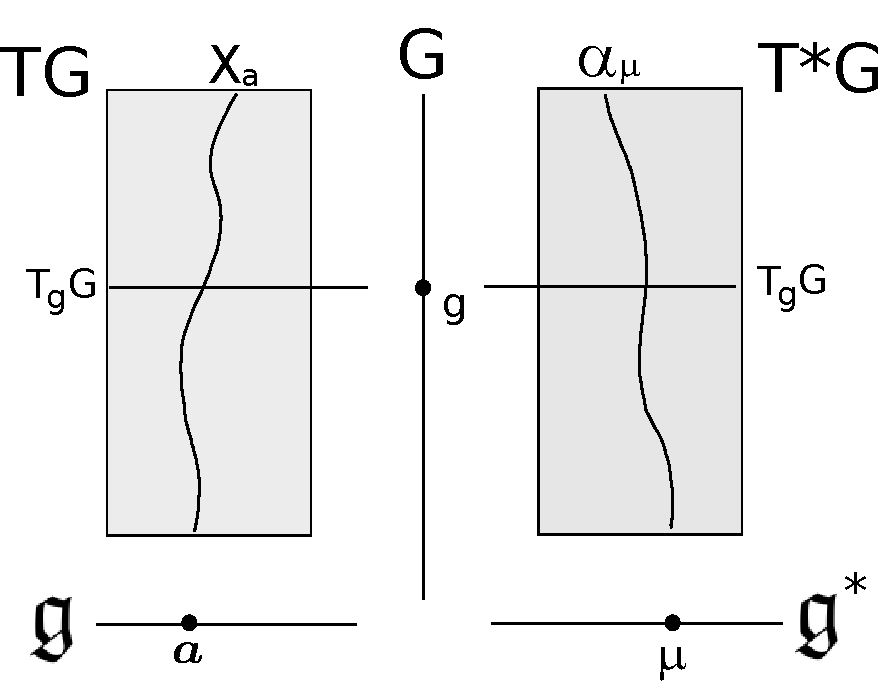
\includegraphics[width=15cm,keepaspectratio]{immagini/Capitolo_V/schemadoppiafibratura.pdf}
			\caption{Schema doppio fibrato}
\end{figure}

\paragraph{In che modo questa proprietà di doppia fibrazione, unita alla proprietà di invarianza della lagrangiana, portano alla riduzione della dinamica del corpo da $TG$ a $\mathfrak{g}$?}$\\$
La risposta è semplice. L'invarianza di $L = L(q^{i}, v^{i})$, dove $v^{i}$ sono le coordinate dei vettori tangenti sulla base invariante (le quasivelocità), implica che $\frac{\partial L}{\partial q^{i}} = 0$. In altre parole $L$ ha valore costante sulle fibre dell'algebra, si riduce quindi ad una funzione $\mathscr{L} : \mathfrak{g}\rightarrow \mathbb{R}$.

La trattazione analitica del paragrafo precedente dimostra come la dinamica filtri in questo caso direttamente sull'algebra, il moto del sistema non è più rappresentato da un moto in $TQ$ ma da una curva in $\mathfrak{g}$. Questo processo è detto di \emph{Riduzione}.

\begin{oss}$\\$
In realtà dalla trattazione precedente si arriva ad un'equazione sul duale dell'algebra, ma questo non è un grande problema, esiste un isomorfismo tra $TG$ e $T^{\ast}G$ realizzato dai momenti canonici del sistema, lo stesso che permette il passaggio dalla formulazione Lagrangiana a quella Hamiltoniana.
$\\$
La proprietà di invarianza di $L$ su $TG$ si trasferisce in una proprietà di invarianza di $H$ su $ T^{\ast}G$ rispetto alla fibrazione indotta dalle 1-forme invarianti a destra.
$\\$
Di conseguenza le equazioni del moto di Hamilton su $T^{\ast}G$ passano al quoziente su $\mathfrak{g}^{\ast}$, si può dimostrare che hanno la forma:
\begin{displaymath}
\dot{l} - ad_{\xi}^{\ast} l = M
\end{displaymath}

\mbox{%
	\begin{minipage}{.18\textwidth}
	\begin{flushleft}
	
\xymatrix{\ar @{} [dr] |{ }
TG \ar[d] \ar[r] & T^{\ast}G \ar[d] \\
\mathfrak{g} \ar[r]
& \mathfrak{g}^{\ast}
}
	\end{flushleft}
	\end {minipage}%	

	\begin{minipage}{.80\textwidth}	\begin{flushleft}
In modo equivalente sarebbe stato possibile passare da $\mathfrak{g}$ a $\mathfrak{g}^{\ast}$ (anzichè da $TG$ a $T^{\ast}G$) usando l'isomorfismo definito dalla riduzione $l(\, v)$ della lagrangiana $L$ su $\mathfrak{g}$.	
	\end{flushleft}
	\end {minipage}
	
	}



\end{oss}






\clearpage
\appendix

\chapter{Strutture Tangenti ad una varietà differenziabile}\label{appendice:1}
 Sia $M$ una generica varietà differenziale, si definiscono:
 
 \begin{defn}[\textbf{Curva Parametrizzata o Cammino}]$\\$
Funzione regolare $\gamma(t): \mathbb{R} \rightarrow M$.
$\\$ Con \emph{regolarità} si intende che la funzione sia di classe $C^{\infty}$ o al limite classe $C^{m}$ dove $m$ è la regolarità delle funzioni di transizione tra le mappe dell'atlante definito sulla varietà.
 \end{defn} 

\begin{defn}[\textbf{Curve Equivalenti}]$\\$
Dati due cammini $\gamma_{1}(t) = \gamma_{2}(t)$ su $M$ questi si dicono \emph{equivalenti} in $x \in M$ se:
\begin{itemize}
\item $\gamma_{\, 1}(0) = \gamma_{\, 2} (0) = x$
\item sia $\phi$ una mappa locale intoro ad $x$, allora:
$$\frac{\textrm{d}}{\textrm{d} t}\bigr(\phi \circ \gamma_{1} \bigr) (0)
= \frac{\textrm{d}}{\textrm{d} t}\bigr(\phi \circ \gamma_{2} \bigr) (0)$$
\end{itemize}
\end{defn} 
\begin{oss}
 Se due curve sono equivalenti in una carta lo sono in tutte. 
 Questo perchè la definizione di varietà differenziale prevede la compatibilità tra carte quindi la regolarità delle funzioni di transizione.
\end{oss} 
$\\$ 
 
Notazione:$\\$ 
D'ora in poi si sottointenderà la scelta di carta locale $\phi$ , pertanto si indicheranno le curve in coordinate. Quindi:
\begin{displaymath}\begin{split}
\bigr(\phi \circ \gamma \bigr) (t) &= \gamma^{i}(t) \\
\frac{\textrm{d}}{\textrm{d} t}\bigr(\phi \circ \gamma \bigr) (0) &= \dot{\gamma}^{i}(0) =v^{i}
\end{split} \end{displaymath} 
In questa forma si interpretano facilmente le curve equivalenti nel punto $x$ come l'insieme dei cammini che hanno la stessa velocità in $x$.
 
 
\begin{defn}[\textbf{Vettore Tangente}]$\\$
Il vettore tangente $V$ nel punto $x \in M$ è la classe di equivalenza di tutte le curve passanti per $x$ con velocità:
$$\dot{\gamma}^{i}(0) = V \in \mathbb{R}$$
 \end{defn} 

\begin{oss}[Identificazione dei vettori come curve.]$\\$
Scegliendo un moto della classe d'equivalenza si può identificare il vettore tangente alla varietà come una curva parametrizzata. Il vettore tangente  è quindi rappresentato dal generico cammino $\gamma(t)$ appartenente alla classe di equivalenza di $V$; quindi tale che:
$$V = \dot{\gamma}(0) $$
\end{oss}
$\\$

\begin{defn}[\textbf{Spazio Tangente in un punto}]$\\$
Lo \emph{spazio tangente} alla varietà $M$ nel punto $x$, indicato con $T_{x}M$, è l'insieme di tutti i vettori tangenti nel punto $x$.
\end{defn} 

\begin{oss}
É possibile dimostrare che gli spazi tangenti $T_{x}M$ hanno la struttura di \emph{spazio vettoriale} per ogni punto $x$ della varietà. 
\end{oss}

$$\\$$ 
\begin{defn}[\textbf{Fibrato Tangente}]$\\$
Il fibrato tangente di M è l'unione disgiunta di tutti gli spazi tangenti ai punti di M:

    $$TM = \coprod_{x\in M}T_xM=\bigcup_{x\in M} \left\{x\right\}\times T_xM$$
\end{defn}


 \begin{defn}[\textbf{Campo vettoriale}]$\\$
Campo vettoriale sulla varietà è una generica mappa $ X: M \rightarrow TM$ tale che:
$$X(z) \in T_{z}M \quad \forall z \in M $$
 \end{defn}

\clearpage
\chapter{Calcolo Differenziale su Una varietà differenziabile}\label{appendice:2}
L'usuale definizione analitica di differenziabilità non si applica direttamente alle funzioni tra varietà in quanto richiede che il dominio sia Euclideo.
$\\$
E' la presenza stessa delle carte che permette di realizzare il calcolo tramite la loro proprietà di associare, almeno localmente, un aperto dello spazio euclideo ad un aperto della varietà.

$\\$
Nello specifico:
 Siano $M,N$ due varietà differenziali, sia $f:M\rightarrow N$ una generica funzione, si definiscono:
 
 \begin{defn}[Differenziabilità]$\\$
 La funzione $f$ è differenziabile nel punto $a \in M$ se: 
 $\\ \forall \phi_{1}$ carta locale di $M$ con dominio contenente $a$ e $\forall \phi_{2}$ carta locale di $N$ con dominio contenente $f(a)$ :

la funzione composta $\phi_{2}\circ f \circ \phi_{1}^{-1} : \mathbb{R}^{m} \longrightarrow \mathbb{R}^{n}$ è differenziabile in $\phi_{1}(a)$ nel senso dell'analisi.
 \end{defn} 
 
$\\$D'ora in avanti le funzioni (f e g(t)) saranno sempre intese rappresentate in carta locale.
 
 \begin{defn}[Differenziale di f]$\\$
 Applicazione lineare $Df(x): T_{x}M \rightarrow T_{f(x)}N$ tale che:
	\begin{displaymath}
Df(x) (v) := \dfrac{\textrm{d}}{\textrm{d}t} f(g(t))|_{t=0} 
	\end{displaymath}
	dove $g(t)$ è un cammino della classe di equivalenza di $v$ tale per cui $g(0) = x $ e $ \dot{g}(0) = \dfrac{\textrm{d}}{\textrm{d}t} (g(t))|_{t=0} = v$
 \end{defn} 
 
Vista la parentela tra vettori e curve è naturale aspettarsi che la definizione di differenziale sia legata a quello di derivata direzionale lungo un cammino. 
 
  \begin{defn}[Derivata direzionale di un campo scalare]$\\$
  Sia $f:M \rightarrow \mathbb{R}$ un campo scalare regolare sulla varietà $M$.
  Nel punto $z \in M$ si definisce $\forall v \in T_{z}M$ la derivata direzionale lungo $v$ come :
  $$ \textrm{d}f(z)\cdot v := \sum_{i}\dfrac{\partial f}{\partial x^{i}} v^{i}$$
	dove $(x^{1},\ldots,x^{k})$ è la rappresentazione di z in una carta locale qualsiasi.  
 \end{defn} 

Quanto definito per un campo scalare e un singolo vettore si può estendere ad un intero campo vettoriale.

 \begin{defn}[Derivata di Lie lungo un campo]$\\$
	Sia $f$ un campo scalare regolare sulla varietà $M$ e sia $X$ un campo vettoriale.
	La derivata di Lie di $f$ lungo $X$ è il campo scalare $X(f): M \rightarrow \mathbb{R}$ tale che:
	$$\forall z \in M \qquad X(f) (z) =  \textrm{d}f(z)\cdot X(z) = X^{i}(x^{1},\ldots,x^{k}) \dfrac{\partial}{\partial x^{i}} f(x^{1},\ldots,x^{k})$$
	dove $(x^{1},\ldots,x^{k})$ è la rappresentazione di z in una carta locale qualsiasi.
 \end{defn} 
 
 \section{L'algebra dei campi vettoriali}
I campi vettoriali ereditano la struttura di Spazio Vettoriale dalle proprietà degli spazi tangenti ma, a differenza dei singoli vettori, è possibile definire su di essi un'operazione di prodotto.

L'introduzione della legge di composizione tra campi vettoriali richiede di invertire il punto di vista su quanto definito fin ora. Invece di vedere la \emph{derivata di Lie} come un operatore associato al campo vettoriale si può identificare il campo vettoriale con la derivata stessa.

Pertanto, sia $X: \mathbb{R}^{n} \rightarrow \mathbb{R}^{n}$ una funzione regolare su M rappresentata in carta locale. $\\$  Si definisce \emph{Campo Vettoriale} su M l'applicazione
$$ X(\cdot) : F \rightarrow F \qquad \textrm{tale che} \qquad X(\cdot) := X^{i}(x^{1},\ldots, x^{n}) \dfrac{\partial}{\partial x^{i}} \cdot$$
dove con $F$ si intende lo spazio dei campi scalari definiti si $M$.

A questo punto la regola di composizione di Campi si interpreta naturalmente come composizione di funzioni:
\begin{displaymath}
\forall f \textrm{ campo scalare} \qquad X(f) ( x^{1},\ldots, x^{n}) = X^{i}\dfrac{\partial}{\partial x^{i}} f( x^{1},\ldots, x^{n}) \textrm{ è ancora un campo scalare} 
\end{displaymath}
Segue che:
\begin{displaymath}
Y \cdot X (f) = Y(X(f)) = Y^{l} \dfrac{\partial}{\partial x^{l}} (X^{i} \dfrac{\partial}{\partial x^{i}} f) = Y^{l} \dfrac{\partial X^{i}}{\partial x^{l}} \dfrac{\partial f}{\partial x^{i}} + Y^{l}X^{i} \dfrac{\partial^{2}}{\partial x^{l} \partial x^{i}}f
\end{displaymath}

Nell'ipotesi che i 2 campi $X, Y$ considerati siano regolari è valido il teorema di Scwhartz, da cui si ottiene che:
\begin{displaymath}
(X \cdot Y - Y \cdot X)(f) = ( X^{l} \dfrac{\partial Y^{i}}{\partial x^{l}} - Y^{l} \dfrac{\partial X^{i}}{\partial x^{l}}) \dfrac{\partial f}{\partial x^{i}}
\end{displaymath}
che ha ancora una volta forma di campo vettoriale.

Quindi l'operazione 
$$[X,Y]= X \cdot Y - Y \cdot X $$  con $X, Y \in\mathfrak{X}(M )$ è chiusa sui campi vettoriali e per le proprietà della regola di composizione di funzioni costituisce un'algebra nel senso espresso dalla definizione [1.4].



\section{Campi F-correlati}
Siano $M,N$ due varietà differenziali, di uguale dimensione.

Sia $f:M\rightarrow N$ un Diffeomorfismo ( funzione di classe $C^{1}$, invertibile e con inversa di classe $C^{1}$), quindi $f$ determina una corrispondenza $1:1$ tra i punti e le curve sulle varietà.

Sia $F$ la rappresentazione in carta locale di $f$, ovvero :
$$ F: \mathbb{R}^{n} \rightarrow \mathbb{R}^{n} \qquad : \qquad y^{i} = F^{i}(x^{1} , \ldots , x^{n})$$

Preso un generico campo $ X^{i}(x^{1}, \ldots, x^{n}) \in \mathfrak{X}(M) $ il differenziale del diffeomorfismo fa corrispondere ad esso un campo vettoriale 
$$ Y^{i}(y^{1}, \ldots, y^{n}) = \dfrac{\partial F^{i}(x^{1} , \ldots , x^{n})}{\partial x^{k}} X^{k} (x^{1} , \ldots , x^{n})$$
sulla varietà $N$.

In tal caso i campi sulle due varietà si dicono F-correlati, ovvero esiste un'applicazione lineare $F_{\ast} : TM \rightarrow TN$ tale per cui per ogni campo X su M corrisponde il campo $Y= F_{\ast}X$ su N di cui l'espessione precendente è la rappresentazione in coordinate.

Questa corrispondenza tra campi vettoriali su varietà ha la proprietà di passare ai commutatori:
\begin{thm}[Passaggio della Correlazione al Commutatore]$\\$
HP:	\begin{itemize}
	\item[-] siano $M,N$ due varietà differenziali e $f:M\rightarrow N$ un Diffeomorfismo tra di esse con $F$ rappresentazione in carta locale.
	\item[-] Presi 2 campi su $M$ di coordinate $X_{1}^{k}(x^{1} , \ldots , x^{n})$ e $X_{2}^{k}(x^{1} , \ldots , x^{n})$.
	\item[-] Presi i campi su $N$ F-Correlati ai campi precedenti $F_{\ast}X_{1}=Y_{1}$ di coordinate $Y_{1}^{k}(y^{1} , \ldots , y^{n})$ e $F_{\ast}X_{2}=Y_{2}$ di coordinate $Y_{2}^{k}(x^{1} , \ldots , x^{n})$. con y=F(x).
	\end{itemize}
	
$\\$ Te: $$[Y_{1},Y_{2}] = F_{\ast}[X_{1},X_{2}]$$ o in coordinate
		$$[Y_{1},Y_{2}]^{i} = \dfrac{\partial F^{i}}{\partial x^{m}}[X_{1},X_{2}]^{m}$$


\proof
Dalle ipotesi si ha che :
$$[Y_{1},Y_{2}]^{i}= Y_{1}^{l}\tiny{(y^{1} , \ldots , y^{n})}\dfrac{\partial Y_{2}^{i}\tiny{(y^{1} , \ldots , y^{n})}}{\partial y^{l}} - Y_{2}^{l}\dfrac{\partial Y_{1}^{i}}{\partial y^{l}} = $$ $$ =
X_{1}^{k}(x^{1} , \ldots , x^{n})\dfrac{\partial F^{l}}{\partial x^{k}}(x^{1} , \ldots , x^{n}) \dfrac{\partial Y_{2}^{i}}{\partial y^{l}}(F^{1}(x) , \ldots , F^{n}(x)) - \ldots$$
ma, derivando la relazione di F-Correlazione
$$Y^{j}\Bigr(F(x)\Bigr) = \dfrac{\partial F^{j}}{\partial x^{m}} X^{m}(x) $$
rispetto $x^{k}$, risulta:

\begin{displaymath}
\dfrac{\partial}{\partial x^{k}}\Bigr(Y^{j} \bigr (F(x) \bigr)\Bigr) = \dfrac{\partial Y^{i}}{\partial y^{l}}\bigr(F(x)\bigr)\dfrac{\partial F^{l}}{\partial x^{k}}(x) = 
\dfrac{\partial F^{i}}{\partial x^{m}} \dfrac{\partial X^{m}}{\partial x^{k}} + \dfrac{\partial^{2} F^{i}}{\partial x^{m} \partial x^{k}} X^{m}
\end{displaymath}

Dunque:

\begin{displaymath}
[Y_{1},Y_{2}]^{i} = X_{1}^{k}\tiny{(x)} \biggr(\dfrac{\partial F^{i}}{\partial x^{m}} \dfrac{\partial X_{2}^{m}}{\partial x^{k}} + \dfrac{\partial^{2} F^{i}}{\partial x^{m} \partial x^{k}} X_{2}^{m}\biggr) - X_{2}^{k}(x)\biggr(\dfrac{\partial F^{i}}{\partial x^{m}} \dfrac{\partial X_{1}^{m}}{\partial x^{k}} + \dfrac{\partial^{2} F^{i}}{\partial x^{k} \partial x^{m}} X_{1}^{m}\biggr) =
\end{displaymath}

\begin{displaymath}
= \dfrac{\partial F^{i}}{\partial x^{m}} (x) \biggr(X^{k}_{1}(x) \dfrac{\partial X_{2}^{m}}{\partial x^{k}}(x) - X^{k}_{2}(x) \dfrac{\partial X_{1}^{m}}{\partial x^{k}}(x) \biggr) = \dfrac{\partial F^{i}}{\partial x^{m}} (x) \Bigr[ X_{1}(x), X_{2}(x)\Bigr]^{m}
\end{displaymath}
Pertanto
\begin{displaymath}
[Y_{1},Y_{2}] = F_{\ast}[X_{1},X_{2}]
\end{displaymath}

\endproof
\end{thm}  
 
\section{L'Algebra dei Campi Invarianti}
Si considerino adesso le due varietà $N$ e $M$ coincidenti con il gruppo di Lie $G$ e si prenda come diffeomorfismo $F$ la traslazione a sinistra $L_{g}: G \rightarrow G$ per un generico elemento $ g \in G$.

Si intende dimostrare che il commutatore fra due campi invarianti è ancora un campo invariante e pertanto lo spazio dei campi invarianti costituisce una sottoalgebra.

Per prima cosa è necessario verificare che il diffeomorfismo considerato preservi l'invarianza dei campi invarianti:


\begin{lem}$\\$
\begin{itemize}
	\item[-] IP: $X_{\xi} (h) = \textrm{d}L_{h}(e) \xi \qquad \xi \in T_{e}G, \forall h \in G$
	\item[-] TE: $ L_{g \ast}\Bigr(X_{\xi}\Bigr) = X_{\xi} $
\end{itemize}
\proof
Si noti innanzi tutto che $ L_{g \ast}\Bigr(X_{\xi}\Bigr)(\cdot)$ rappresenta un campo sulla varietà $G$, pertanto:
\begin{displaymath}
L_{g \ast}\Bigr(X_{\xi}\Bigr)(gh) = \textrm{d}L_{g}(h) X_{\xi}(h) = \textrm{d}L_{g}(h) \textrm{d}L_{h}(e) \xi
\end{displaymath}
ma per la legge di prodotto gruppale le due traslazioni, anche quelle vettoriali, si compongono:
\begin{displaymath}
L_{g \ast}\Bigr(X_{\xi}\Bigr)(gh) = \textrm{d}L_{g h}(e) \xi = X_{\xi} (g h)
\end{displaymath}
\endproof
\end{lem} 
A questo punto, ricordando il risultato del paragrafo precedente:
$$[X,Y] \in \mathfrak{X}(G) \qquad \forall X,Y \in \mathfrak{X}(G)$$
segue che:

\begin{table}[h!]
\begin{center}
\begin{tabular}{rcccl}
$L_{g \ast} \bigr[ X_{\xi}, X_{\eta}]$& = & $\bigr[L_{g \ast}X_{\xi}, L_{g \ast}X_{\eta} \bigr] $ & = & $\bigr[X_{\xi}, X_{\eta}] $\\
 & Teorema A.2.1 & & Lemma A.2.2 & \\
\end{tabular}
\end{center}
\end{table} 
Di conseguenza il commutatore dei campi è chiuso rispetto ai campi invarianti quindi lo spazio $\mathfrak{X}^{L}(G) $ dei campi invarianti a sinistra sul gruppo di Lie $G$ costituisce una sottoalgebra.


\clearpage
\begin{thebibliography}{99}
\bibitem{Holm} D.D. Holm; T. Schmah; C. Stoica \, \emph{Geometric Mechanics and Symmetry}

\bibitem{Ratiu} J.E. Marsden; T.S. Ratiu \, \emph{Introduction to Mechanics and Symmetry}, 2nd.ed

\bibitem{Corben} H.C. Corben; P. Stehle \emph{Classical Mechanics}, 2nd.ed.

\bibitem{lagrange} J.L. Lagrange \, \emph{Théorie de la libration de la Lune et des autres phénomès qui dependent de la figure non spherique de cette planète.} {\small(Mémoires de l'académie des sciences de Berlin, 1780)}

\bibitem{Poincare} H. Poincarè \, \emph{Sur une forme nouvelle des équations de la mécanique} {\small( C.R.A.S 1901 )}
%prensenta l'equazione e-p nella forma data con i coefficienti di struttura

\bibitem{Eulero1} L. Eulero \, \emph{Decouverte d'un nouveau principe de Mécanique } {\small( Mémoires de l'académie des sciences de Berlin 6, 1752, pp. 185-217 ) }
%fanno la comparsa le equazioni di eulero per il moto del corpo rigido con punto fisso

\bibitem{Eulero2} L. Eulero \, \emph{Du mouvement d'un corps solide quelconque lorsq'il tourne autour d'un axe mobile} {\small(Memoires de l'academie des sciences de Berlin 16, 1767, pp. 176-227 )}

\bibitem{Hamel} G. Hamel \, \emph{Theoretische Mechanik} {\small(ed. Springer, 1946 )}
%parla dell'equazione centrale, le da il nome

\bibitem{Lurie} L. Lur'É \, \emph{Mécanique Analytique} {\small(Librarie universitaire Lovanio. 1964)}
%cita hamel e presenta l'equazione centrale di lagrange

\end{thebibliography}
\end{document}




